\documentclass[twoside,10pt,a4paper]{article}
% \usepackage[latin1]{inputenc}
\usepackage[utf8]{inputenc} % usually not needed (loaded by default)
\usepackage[T1]{fontenc}
% \usepackage{amsmath}
\usepackage{amsfonts}
% \usepackage{amssymb}
\usepackage{amsmath,amsthm,amssymb}
\usepackage{graphicx}
\usepackage{hyperref}
% \usepackage{courier}
\usepackage{placeins}
\usepackage{fancyhdr}
\usepackage{color}
% \usepackage{xcolor}
\usepackage{listings}
\usepackage{geometry}
\usepackage{tabularx}
\usepackage[table]{colortbl}
\usepackage{placeins}
% \usepackage{cite}
\usepackage{subcaption}
\usepackage{lipsum}
\usepackage{titlesec}
\usepackage{dsfont}
\usepackage{parskip}
\usepackage{ragged2e}
\usepackage{soul}
\usepackage{tablefootnote}
\usepackage{epigraph}
\usepackage{setspace}
\usepackage[backend=biber, sorting=none]{biblatex}
\addbibresource{mybib.bib}
\usepackage[skip=8pt,labelfont=bf, font=sf]{caption}
	\DeclareCaptionFont{myfont}{\fontfamily{\sfdefault}\selectfont}

\hypersetup{
	colorlinks   = True,
	citecolor    = blue,
	linkcolor	 = blue,
}

% \geometry{letterpaper, portrait, margin=1in}
% \geometry{a4paper,margin=15mm,bindingoffset=25mm,heightrounded,}
\geometry{a4paper,margin=25mm}

\usepackage[dvipsnames]{xcolor}
\definecolor{lightgray}{rgb}{.93,.93,.93}
\definecolor{darkgray}{rgb}{.4,.4,.4}
\definecolor{purple}{rgb}{0.65, 0.12, 0.82}

\usepackage{array}
\newcolumntype{?}{!{\vrule width 1.5pt}}

\usepackage{helvet}
\usepackage{times}

\titleformat{\chapter}[display]
  {\normalfont\sffamily\huge\bfseries} % \color{blue}
  {\chaptertitlename\ \thechapter}{20pt}{\Huge}
\titleformat{\section}
  {\normalfont\sffamily\huge\bfseries} % \color{cyan}
  {\thesection}{1em}{}
 \titleformat{\subsection}
  {\normalfont\sffamily\Large\bfseries} % \color{cyan}
  {\thesubsection}{1em}{}
 \titleformat{\subsubsection}
  {\normalfont\sffamily\large\bfseries} % \color{cyan}
  {\thesubsubsection}{1em}{}
\renewenvironment{abstract}
 {\par\noindent\Huge\textbf{\abstractname.}\\\vspace{1em}\ignorespaces}
 {\par\medskip} 

% \renewcommand*\abstractname{Abstract\hfill}
% \renewcommand{\familydefault}{\sfdefault}


\def \lineheight {1.5pt}

\makeatletter
   \def\vhrulefill#1{\leavevmode\leaders\hrule\@height#1\hfill \kern\z@}
\makeatother

\usepackage{caption}
    \DeclareCaptionType{mycapequ}[][List of equations]
    \captionsetup[mycapequ]{labelformat=empty}

\usepackage{inconsolata}

\lstset{
	language=Matlab,
	backgroundcolor=\color{lightgray},
	keywordstyle=\color{blue}\bfseries,
	stringstyle=\color{red}\ttfamily,
	commentstyle=\color{ForestGreen}\ttfamily,
	identifierstyle=\color{black},
	extendedchars=true,
	% basicstyle=\footnotesize\ttfamily,
	basicstyle=\normalsize\fontencoding{T1}\ttfamily,
	showstringspaces=false,
	showspaces=false,
	numbers=left,
	numberstyle=\footnotesize,
	numbersep=9pt,
	tabsize=2,
	breaklines=true,
	showtabs=false,
	captionpos=b
}

\lstset{
	language=Python,
	backgroundcolor=\color{lightgray},
	keywordstyle=\color{blue}\bfseries,
	stringstyle=\color{red}\ttfamily,
	commentstyle=\color{ForestGreen}\ttfamily,
	identifierstyle=\color{black},
	extendedchars=true,
	% basicstyle=\footnotesize\ttfamily,
	basicstyle=\normalsize\fontencoding{T1}\ttfamily,
	showstringspaces=false,
	showspaces=false,
	numbers=left,
	numberstyle=\footnotesize,
	numbersep=9pt,
	tabsize=2,
	breaklines=true,
	showtabs=false,
	captionpos=b
}

\fancypagestyle{firstpage}{%
  \fancyhf{}% clear default for head and foot
  % \rfoot{\textbf{Page \thepage}}
  % \lfoot{\textbf{\today}}
  \renewcommand{\headrulewidth}{0pt}
}
\fancypagestyle{blank}{%
	\fancyhf{}
	\renewcommand{\headrulewidth}{0pt}
}

\fancypagestyle{nohdr}{%
	\fancyhf{}
	\renewcommand{\headrulewidth}{0pt}
	% \rfoot{\fontfamily{\sfdefault}\selectfont\textbf{Page \thepage}}
	\fancyfoot[LE,RO]{\fontfamily{\sfdefault}\selectfont \textbf{Page \thepage}}
}

\renewcommand{\headrulewidth}{1pt}% 2pt header rule


% \fontfamily{\sfdefault}\selectfont
	% \large\fontfamily{\rmdefault}\selectfont 

\setlength{\parskip}{12pt} % 1ex plus 0.5ex minus 0.2ex}
\setlength{\parindent}{0pt}
% \linespread{1.5}
\onehalfspacing

\DeclareMathOperator*{\argmin}{argmin}

\usepackage{tikz}
\usepackage{enumitem}
\newcommand*\mycirc[1]{%
\begin{tikzpicture}[baseline=(C.base)]
\node[draw,circle,inner sep=1pt,minimum size=3ex](C) {#1};
\end{tikzpicture}}

\pagestyle{fancy}
% \renewcommand{\sectionmark}[1]{\markboth{ #1}{}}
% \renewcommand{\subsectionmark}[1]{\markboth{\thesection\ #1}{\thesubsection\ #1}}
\fancyhf{}
% \rhead{\fontfamily{\sfdefault}\selectfont \textbf{\rightmark}}
% \lhead{\fontfamily{\sfdefault}\selectfont \textbf{Thesis}}
% \rfoot{\fontfamily{\sfdefault}\selectfont \textbf{Page \thepage}}
% \lfoot{\fontfamily{\sfdefault}\selectfont \textbf{Cole Nielsen}} % \today
\fancyhead[LE,RO]{\fontfamily{\sfdefault}\selectfont \textbf{\rightmark}}
% \fancyhead[RE,LO]{Guides and tutorials}
% \fancyfoot[CE,CO]{\rightmark}
\fancyfoot[LE,RO]{\fontfamily{\sfdefault}\selectfont \textbf{Page \thepage}}
\title{\textbf{}}
\date{}

\sloppy\RaggedRight\raggedbottom
\begin{document}	
		% \maketitle 
	% \renewcommand{\familydefault}{\sfdefault}
	\thispagestyle{firstpage}
	\fontfamily{\sfdefault}\selectfont 
	
\includegraphics[width=0.5\linewidth]{logo_ntnu_eng_black.png} \\
	\vspace{8em}
	\huge Ultra Low Power Frequency Synthesizer\\	
	\vspace{3em}
	\huge \textbf{Cole Nielsen}\\
	\vspace{12em}
	\large%
	%Electronic Systems Design, Master's Thesis\\
	Master's thesis in Electronic Systems Design\\
	\vspace{4pt}
	\FloatBarrier

	\def\arraystretch{1.3}
	\setlength{\tabcolsep}{1em}
	\begin{tabular}{@{} l  l}
	Submission date: & June 2020\\
	Supervisor: & Trond Ytterdal, IET\\
	Co-supervisor: & Carsten Wulff, IET\\
	\end{tabular} \\
	\FloatBarrier
	\vspace{3em}
	Norwegian University of Science and Technology \\ 
	\vspace{4pt}Department of Electronic Systems\\
	
	% \begin{center}
	% 	\large
	% 	\begin{tabular}{ l r }
	% 		\textbf{Name} & Cole Nielsen \\
	% 		\textbf{Assigned N$^\textbf{\textnormal{o}}$} & 13 \\
	% 		\textbf{Term} & Autumn 2018\\
	% 		\textbf{Instructor} & Guennadi Kouzaev\\
	% 	\end{tabular}
	% \end{center}
	% \vspace{2em}
	% \vhrulefill{\lineheight}
	\pagebreak
	% \thispagestyle{blank}
	% \null\pagebreak

	% % % % % % % % % % % % % % % % % % % % % % % % % % % % % % % % % % % % 
	% Abstract
	\justify
	\setcounter{page}{1}
	% \pagebreak
	\thispagestyle{nohdr}
	\large\fontfamily{\sfdefault}\selectfont \		
	\begin{abstract} \large\fontfamily{\rmdefault}\selectfont \
		
		\vspace{-2em}A power and jitter FOM state of art integer-N all digital phase locked loop (ADPLL) frequency synthesizer implemented in a commercially available 22nm FD-SOI process is presented in this paper. Achieved was a power consumption of 95 $\mu$W with 12 oscillator phases at 816 MHz, a jitter FOM of -225 dB, and an active area of 0.00365 mm$^2$. This was obtained through an emphasis on power reducing architectural choices for application to low duty cycle wake up receivers (WUR), utilizing low complexity, bias and reference-free circuits. Included is a novel, pseudo-differential voltage controlled ring oscillator using FD-SOI backgates to implement both frequency tuning and differential behavior. This voltage controlled oscillator achieves high frequency tuning gain linearity with rail-to-rail input range, while using no static current biasing. The proposed oscillator enables 2.448 GHz IQ sampling through oversampling at the 1/3 subharmonic (816 MHz). Capacitive DACs are used to provide digital control to the oscillator with minimum power draw. A low complexity band-bang phase detector (BBPD) and an all digital proportional-integral (PI) loop filter with divider-free operation implement the remaining portions of the PLL. Furthermore, a mathematical model regarding the novel oscillator is introduced, a phase noise optimization theory is presented for PI loop-filter design in BBPD-PLLs, and theory regarding DAC resolution determination is also outlined. Finally, a theoretical limit for achievable PLL FOM$_{jitter}$ in the proposed design is established.
	\end{abstract}
	% \section*{Abstract}
	% fjdsfkajjlkf

	% % % % % % % % % % % % % % % % % % % % % % % % % % % % % % % % % % % % 
	% Preface
	\pagebreak
	% \thispagestyle{nohdr}
	% \null\pagebreak
	\thispagestyle{nohdr}
	\large\fontfamily{\sfdefault}\selectfont 
	\Huge\textbf{Preface.}\\
	\epigraph{Simplicity is the ultimate sophistication.}{\textit{Leonardo da Vinci}}
	\large\fontfamily{\rmdefault}\selectfont 
	\vspace{1em}
	I would like to thank my advisors Trond Ytterdal and Carsten Wulff for providing me the opportunities to further my knowledge and experience in the dark arts of circuit design.

	\par I also thank my family for their continual open support of my life endeavors.


	\vspace{6em}
	Cole Nielsen 

	\vspace{0em}
	June 2020, Trondheim.

	% % % % % % % % % % % % % % % % % % % % % % % % % % % % % % % % % % % % 


	% % % % % % % % % % % % % % % % % % % % % % % % % % % % % % % % % % % % 
	% Project Description
	\pagebreak
	% \thispagestyle{nohdr}
	% \null\pagebreak
	\thispagestyle{nohdr}
	\large\fontfamily{\sfdefault}\selectfont 
	\Huge\textbf{Problem description.}\\
	% \vspace{1em}
	\large\fontfamily{\rmdefault}\selectfont 
	
	The intent of this project is to develop an ultra low power, integer-N all-digital PLL (ADPLL) frequency synthesizer for application to wake up receiver (WUR) radio circuits. The target technology is a commercially available fully-depleted silicon on insulator (FD-SOI) process with 22nm node size. The implemented PLL is intended for use in duty cycled WUR circuit applications, with on the order of 1\% active time. Due to the duty cycled requirement, the design must enable rapid locking times such that fast wake-up from a sleep state can be achieved. The required specifications for this PLL design are given in table \ref{reqs}. Given the radio application of the work, a direct phase noise requirement is not provided, rather, performance is constrained in terms of the modulation scheme and target bit error rate of the radio system. Therefore, the implemented PLL must enable satisfactory operation of this radio system.
		\begin{table}[htb!]
			\centering
			\def\arraystretch{1.5}		
			\setlength\arrayrulewidth{1pt}
			\setlength{\tabcolsep}{1em} % for the horizontal padding
			\fontfamily{\sfdefault}\selectfont 
			\begin{tabular}{|l|r|l|}	
				\hline 
				\rule[-1ex]{0pt}{2.5ex} \cellcolor{gray!40}\textbf{Parameter} & \cellcolor{gray!40}\textbf{Specification} & \cellcolor{gray!40}\textbf{Unit}\\ 
				\hline 
				\rule[-1ex]{0pt}{2.5ex} Power & $\leq$ 100 &  $\mu$W  \\ 
				\hline 
				\rule[-1ex]{0pt}{2.5ex} Reference frequency\tablefootnote{Frequencies derived from the reference, for example through division, are also acceptable.} &  32  &  MHz  \\ 
				\hline 
				\rule[-1ex]{0pt}{2.5ex} Synthesized frequency\tablefootnote{Or equivalent through sampling.} & 2.448 &  GHz  \\ 
				\hline 
				\rule[-1ex]{0pt}{2.5ex} BER\tablefootnote{At 250 Kbps with symbols encoded as $\pm2\pi$ phase shifts.} & $\leq$ 10$^{-3}$ & \\ 
				\hline 
				\rule[-1ex]{0pt}{2.5ex} Lock time & $\leq$ 5 & $\mu$s  \\ 
				\hline 
				% \rule[-1ex]{0pt}{2.5ex} FOM$_{\Phi n}$\tablefootnote{ FOM$_{\Phi n} = 10\log_{10}\left(\frac{\sigma_{t_j}^2}{(\textnormal{1 s})^2}\cdot\frac{\textnormal{Power}}{\textnormal{1 mW}}\right)$, where $\sigma_{t_j}$ is the measured RMS timing jitter of the PLL.} & $\leq$ -230 & dB  \\ 
				% \hline 
			\end{tabular} 
			\caption{Design required specifications.}
			\label{reqs}
		\end{table} 
	\large\fontfamily{\rmdefault}\selectfont 
	\par This work is in part a continuation of the author's previous work \cite{Me} on the optimization and simulation of integer-N ADPLLs, which focused on automation of loop filter design. This previous work has motivated the architectural choices of this work, particularly the usage of a bang-bang phase detector with a proportional-integral (PI) controller based loop filter. This architecture was found to be advantageous in terms of complexity and optimizability, providing for a known good starting point on this project.

	% % % % % % % % % % % % % % % % % % % % % % % % % % % % % % % % % % % % 
	% % Preface
	% \pagebreak
	% \thispagestyle{nohdr}
	% \null\pagebreak
	% \thispagestyle{nohdr}
	% \large\fontfamily{\sfdefault}\selectfont 
	% \Huge\textbf{Preface.}\\
	% \vspace{1em}
	% \large\fontfamily{\rmdefault}\selectfont 
	% \lipsum[1]

	% % % % % % % % % % % % % % % % % % % % % % % % % % % % % % % % % % % % 
	% Contents, list of tables and figures
	\fontfamily{\sfdefault}\selectfont 
	\thispagestyle{nohdr}
	% \null\pagebreak
	% \thispagestyle{nohdr}
	\null\pagebreak
	\tableofcontents
	\pagebreak
	\listoffigures
	\listoftables

	% \vhrulefill{\lineheight}

	\fontfamily{\rmdefault}\selectfont 
	% % % % % % % % % % % % % % % % % % % % % % % % % % % % % % % % % % % % 
	% Abbreviations
	\pagebreak
	\FloatBarrier
	\section*{Abbreviations.}
	\begin{table}[htb!]
	\renewcommand*{\arraystretch}{1.30}\large
	\begin{tabular}{@{}ll}
		\textbf{\textsf{ADPLL}}	&	All digital phase locked loop \\
		\textbf{\textsf{BBPD}}	&	Bang-bang phase detector \\
		\textbf{\textsf{BOX}}	&	Burried-oxide \\
		\textbf{\textsf{BW}}	&	Bandwidth \\
		\textbf{\textsf{CDAC}}	&	Capacitive digital to analog converter \\
		\textbf{\textsf{CDF}}	&	Cumulative distribution function \\
		\textbf{\textsf{CI}}	&	Confidence interval \\
		\textbf{\textsf{CLK}}	&	Clock \\
		\textbf{\textsf{CM}}	&	Common mode \\
		\textbf{\textsf{CMOS}}	&	Complementary metal oxide semiconductor \\
		\textbf{\textsf{CMRR}}	&	Common mode rejection ratio \\
		\textbf{\textsf{CNR}}	&	Carrier to noise ratio \\
		\textbf{\textsf{DAC}}	&	Digital to analog converter \\
		\textbf{\textsf{DC}}	&	Direct current \\
		\textbf{\textsf{DCO}}	&	Digitally controlled oscillator \\
		\textbf{\textsf{DFF}}	&	D flip flop \\
		\textbf{\textsf{DIV}}	&	Divider \\
		\textbf{\textsf{DNL}}	&	Differential non-linearity \\
		\textbf{\textsf{FDSOI}}	&	Fully depleted silicon on insulator \\
		\textbf{\textsf{FET}}	&	Field effect transistor \\
		\textbf{\textsf{FOM}}	&	Figure of merit \\
		\textbf{\textsf{FSK}}	&	Frequency shift keying \\
		\textbf{\textsf{FSM}}	&	Finite state machine \\
		\textbf{\textsf{HVTPFET}}	&	High threshold voltage PFET \\
		\textbf{\textsf{IIR}}	&	Infinite impulse response \\
		\textbf{\textsf{INL}}	&	Integral nonlinearity \\
		\textbf{\textsf{ISF}}	&	Impulse sensitivity function \\
		\textbf{\textsf{KDCO}}	&	DCO Gain \\
		\textbf{\textsf{LC}}	&	Inductor-capacitor \\
		\textbf{\textsf{LF}}	&	Loop filter \\
		\textbf{\textsf{LO}}	&	Local oscillator \\
		\textbf{\textsf{LSB}}	&	Least significant bit \\
		\textbf{\textsf{LVTNFET}}	&	Low voltage threshold NFET \\
		\textbf{\textsf{MMSE}}	&	Minimum mean squared error \\
		\textbf{\textsf{MOSFET}}	&	Metal oxide semiconductor filed effect transistor \\
	\end{tabular}
	\end{table}
	\begin{table}[htb!]
	\renewcommand*{\arraystretch}{1.30}\large
	\begin{tabular}{@{}ll}
		\textbf{\textsf{MSE}}	&	Mean squared error \\
		\textbf{\textsf{NFET}}	&	N-channel field effect transistor \\
		\textbf{\textsf{NMOS}}	&	N-channel metal oxide semiconductor \\
		\textbf{\textsf{OOK}}	&	On-off keying \\
		\textbf{\textsf{OTW}}	&	Oscillator tuning word \\
		\textbf{\textsf{PD}}	&	Phase detector \\
		\textbf{\textsf{PDF}}	&	Probability distribution function \\
		\textbf{\textsf{PFET}}	&	P-channel FET \\
		\textbf{\textsf{PI}}	&	Proportional-integral \\
		\textbf{\textsf{PID}}	&	Proportional-integral-derivative \\
		\textbf{\textsf{PLL}}	&	Phase locked loop \\
		\textbf{\textsf{PMOS}}	&	P-channel metal oxide semiconductor \\
		\textbf{\textsf{PN}}	&	Phase noise \\
		\textbf{\textsf{PSD}}	&	Power spectral density \\
		\textbf{\textsf{PSK}}	&	Phase shift keying \\
		\textbf{\textsf{PVT}}	&	Process \\
		\textbf{\textsf{RC}}	&	Resistor-capacitor \\
		\textbf{\textsf{RMS}}	&	Root mean squared \\
		\textbf{\textsf{RO}}	&	Ring oscillator \\
		\textbf{\textsf{RST}}	&	Reset \\
		\textbf{\textsf{RVT}}	&	Regular voltage threshold \\
		\textbf{\textsf{SLVTNFET}}	&	Super-low voltage threshold NFET \\
		\textbf{\textsf{SNR}}	&	Signal to noise ratio \\
		\textbf{\textsf{SOI}}	&	Silicon on insulator \\
		\textbf{\textsf{SSB}}	&	Single side band \\
		\textbf{\textsf{TDC}}	&	Time to digital converter \\
		\textbf{\textsf{TF}}	&	Transfer function \\
		\textbf{\textsf{TSPC}}	&	True single phase circuit \\
		\textbf{\textsf{UTBB}}	&	Ultra-thin body BOX \\
		\textbf{\textsf{VCO}}	&	Voltage controlled oscillator \\
		\textbf{\textsf{WUC}}	&	Wake up call \\
		\textbf{\textsf{WUR}}	&	Wake up receiver \\
	\end{tabular}
	\end{table}

	% \FloatBarrier\pagebreak
	\null

	% % % % % % % % % % % % % % % % % % % % % % % % % % % % % % % % % % % % 
	\pagebreak\FloatBarrier

	\section{Introduction}\label{intro}
	Phase locked loops (PLLs) are the fundamental building block to virtually all wired and wireless communication systems of today. To meet industrial demands of continual and uncompromising advancement of communication system performance, e.g. higher data rates, lower power, it is paramount that PLL performance is continually improved. Of perpetually growing importance is the application of PLLs to radios in battery powered mobile and internet of things (IoT) devices, for which reduction of power is highly sought after. A recent approach to reducing power consumption in such wireless applications is through usage of wake up receivers (WURs). These are ultra low power, low data rate radio receivers that listen for requests (i.e. "wake up calls", or WUCs) for activity from some external source. Upon a WUC, the device powers on and activates a higher powered radio supporting faster data rates for only the time required. In devices that are inactive for substantial periods of time, waiting for requests for activity (e.g. as with sensor networks or wireless headphones), such a scheme can enable great power reduction, for example achieving 4.5 nW in \cite{Jiang2017} and 365 nW in \cite{Sadagopan2017} for 2.4 GHz band WUC reception. When this is compared to utilizing a full data rate receiver to poll the radio spectrum for activity requests, which for a state of art Bluetooth design may draw on the order of 1.9 mW \cite{Tamura2020}, it is seen that upwards of $10^6$ improvement in power is obtainable, undoubtedly reducing the overall achievable system power consumption for many wireless applications.

Thus, in this work, the design of a low power PLL which enables WUR applications is considered. Ultra low power consumption has been achieved with PLL-less on-off keying receivers, for example accomplishing 4.5 nW with 0.3 kbps of data at 2.4 GHz in \cite{Jiang2017}. However, this work will be catered to PLL-based designs that maintain backwards-compatibility with FSK and PSK modulation schemes supported by existing wireless standards such as 802.15.4, WiFi and Bluetooth. A review of current literature shows that the state of art within ultra low power PLLs in the 2.4 GHz band regime achieve power consumption on the order of hundreds of $\mu$W, for example 170 $\mu$W in \cite{Zhang2019}, and 265 $\mu$W in \cite{Liu2019}. Therefore, to advance the boundary of the current state of art, this work seeks to set a new record for PLL power consumption, namely $\leq$ 100 $\mu$W for use in 2.4 GHz band radio operation. Furthermore, an attempt will be made to minimize implemented area of the PLL. Current state of art for PLL area rests in the sub-0.01 mm$^2$ regime, with as small as 0.0036 mm$^2$ being seen in 5nm process technology \cite{Liu2020}. It will be attempted to obtain a similar area to the current state of art.
% To meet these goals, a PLL design methodology is described in this work, favoring minimization of overall complexity,educing current braches and circuit area, whilst yielding high performance on a given power budget.


 A brief outline of the paper is as follows. An introduction to PLL and FD-SOI theory is in section \ref{theory}. The undertaken PLL design is discussed in sections \ref{pll_arch}-\ref{behav_sim}. Simulation results of the implemented design are in section \ref{results}. Comparison to the state of art and general discussion regarding this work are in section \ref{disco}. Finally, section \ref{conclusion} concludes. 
%
%
% Phase locked loops are extraordinarily useful frequency synthesizers that are vital to the operation of virtually all wThe trend towards increasingly lower power wireless devices poses an acute need to reduce PLL power consumption. This is a challenge as PLLs typically rank among the highest power consuming components of a radio, and are necessarily so to limit oscillator phase noise. A sampling of literature on ultra-low power 2.4GHz radios finds oscillator power consumption as a portion of total radio consumption to be 53\% for the receiver in \cite{regulagadda_2018}, 88\% of the transmitter in \cite{shi_2019}, 52\% of the transmitter in \cite{chen_2019}, and 50\% of the receiver in \cite{pengg_2013}. Reducing analog PLL power consumption can be a prohibitive challenge as the performance of analog loop filters degrade as a result of unavoidably lower charge pump current. However, recent CMOS process nodes with minimum gate lengths as small as 7nm allow for all-digital loop filters and PLLs to be a possible alternative to analog designs due to increasingly low power consumption associated with their implementation. Digital loop-filters have the unique advantage where they can be scaled indefinitely as process nodes advance, suffering no loss in performance, while also having greatly reduced sensitivities to process, voltage, temperature (PVT) variations compared to analog implementations.
%
%
% Thus, in this paper, a new framework, \texttt{pllsim}, written in Python\footnote{Python Software Foundation \url{https://www.python.org/}.} is introduced (this framework is available on GitHub\footnote{\texttt{pllsim} codebase: \url{https://github.com/nielscol/pllsim}.}), which uniquely addresses issues of ultra-low power ADPLL design. Specifically, design of integer-N type PLLs is focused on, as the impetus of this work is an integer-N PLL design project. Topics presented are (a) automatic design and optimization of ADPLL loop filters given target system and component level specifications for the PLL, and (b) behavioral time domain PLL simulation for accurate analysis and verification of loop filter and PLL performance, with an integrated Monte-Carlo sampling variation analysis engine. Due to high phase noise associated with low power design, the optimization approach introduced in this paper focuses on the minimization of total integrated phase noise power to allow for maximum PLL performance on a given power budget.
%

\vspace{1em}

\subsection{Main Contributions}
% \vspace{-0.8em}
\begin{enumerate}[itemsep=0pt,label=\protect\mycirc{\arabic*}]
	\setlength\itemsep{-0.8em}
	\item Implementation of a sub-100 $\mu$W ultra-low power, 0.00365 mm$^2$ area CMOS PLL in a 22nm FD-SOI process technology, with state of art FOM$_{jitter}$ within its power regime, and comparable area to the current state of art.
	\item Presentation of a novel pseudodifferential ring oscillator circuit topology and theory of operation, utilizing FD-SOI backgates to implement both frequency tuning and differential operation.
	\item Realization of a highly linear voltage controlled oscillator with rail-to-rail input range. 
	\item Loop filter optimization theory for proportional-integral controller bang-bang phase detector PLLs with noisy phase detectors.
	\item Theoretical figure for the FOM$_{jitter}$ performance limit of proportional-integral controller bang-bang phase detector PLLs.
	\item DAC resolution and oscillator frequency gain optimization theory.
	\item A novel pseudodifferential buffer presenting common mode rejection characteristics.
	\item Implementation of low power CDACs.
	\item Implementation of a low power bang-bang phase detector.
	\item Implementation of a low power digital loop filter.
	\item Demonstration of bias current and reference free PLL design.
\end{enumerate}

	\pagebreak\FloatBarrier


	\pagebreak
	\section{Redefining Requirements}
	With the purpose of this work to be applied to a radio system, the high level requirements of the PLL are constrained by the performance requirements of end use radio system. The target for this work is to enable a bit error rate of $\leq 10^{-3}$ using a slightly modified Gaussian minimum shift keying (GMSK) \cite{rappaport_wireless_2002} modulation scheme. The transmitted signal is to have a nominal 1 Mbps data rate and a bandwidth-time (BT) product of 0.5, where 1 and 0 respectively are encoded as $\pm \pi/2$ phase shift per symbol in the signal. The receiver, however, is to be operated at lower symbol rate of 250 kbps. To match data rates, the transmitter therefore must transmit four identical symbols at 1 Mbps to encode one symbol as seen by the receiver. The result of such a scheme is that one received symbol will be constituted by a phase shift of $\pm 2\pi$, or a full rotation of the signal constellation, which increases the detectability of the received signal. To determine PLL requirements for this scheme, a simulation of bit error rate versus carrier-to-noise ratio (CNR) of the modulated signal has been performed, with the results in figure \ref{fig:ber_cnr}. It is found that for a BER of $10^{-3}$, a minimum of 6.4 dB of CNR is required for the radio system. In the case of this work, where the PLL is constrained to ultra low power, it is now assumed that the PLL will be the limiting factor in terms of noise in the implemented radio system. Therefore, the CNR of the oscillator, that is the ratio of the main tone power to phase noise power, must be at least the determined value of 6.4 dB. To provide a slight margin due to the inevitable presence of other noise sources in the radio system, a specification for CNR $\geq$ 10 dB for the PLL has been selected. It is more typical to define PLL performance in terms of root mean square (RMS) jitter, accordingly table \ref{tab:pll_specs} contains the final translated requirements of the PLL to meet the intended radio system performance targets. Another relevant requirement for the PLL is it must enable IQ sampling of RF signals at 2.448 GHz.




\begin{figure}[htb!]
	\begin{floatrow}
	\ffigbox{%
		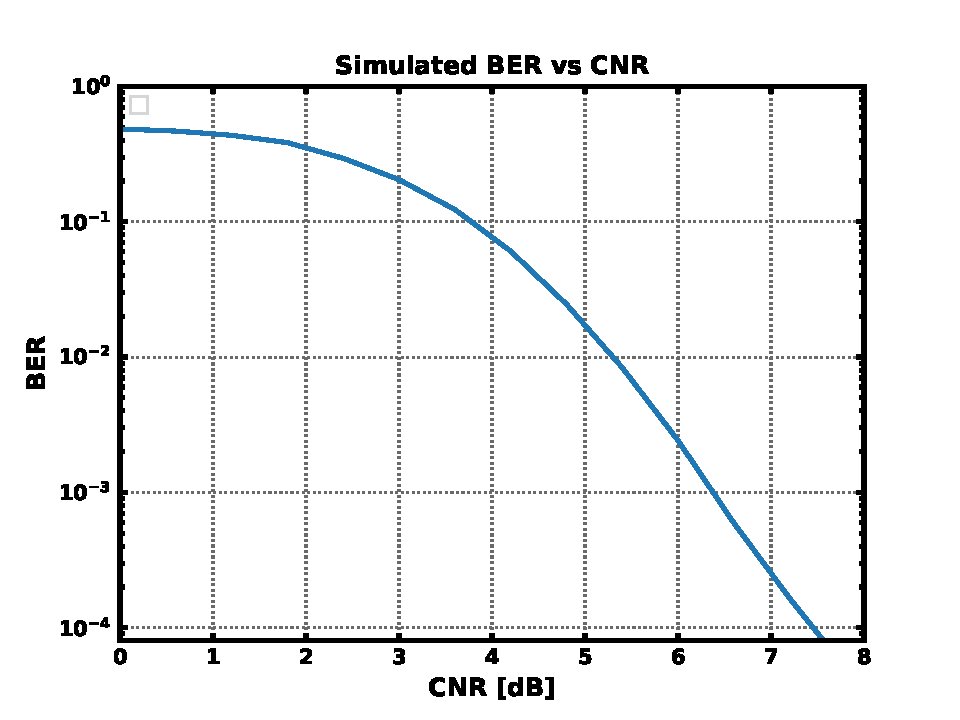
\includegraphics[width=0.5\textwidth, angle=0]{./figs/theory/ber_cnr}
	}{%
	    \caption{Bit error rate versus carrier to noise ratio of targeted radio system modulation scheme.}
	    \label{fig:ber_cnr}
	}
	\capbtabbox{%
		\def\arraystretch{1.5}		
		\setlength\arrayrulewidth{0.75pt}
		\setlength{\tabcolsep}{1em} % for the horizontal padding
		\begin{tabular}{|c|c|c|}
			\hline 
			\rule[-1ex]{0pt}{2.5ex} \cellcolor{gray!40}\textbf{Parameter} & \cellcolor{gray!40}\textbf{Value} & \cellcolor{gray!40}\textbf{Units}\\ 
			\hline 
			\rule[-1ex]{0pt}{2.5ex} \textbf{CNR} (at 2.448 GHz) & $\geq$ 10 & dB \\ 
			\hline 
			\rule[-1ex]{0pt}{2.5ex} \textbf{RMS Jitter } &  $\leq$ 20.56 & ps  \\ 
			\hline 
			\rule[-1ex]{0pt}{2.5ex} \textbf{Frequency} &  2.448 & GHz  \\ 
			\hline 
			\rule[-1ex]{0pt}{2.5ex} \textbf{Power} &  $\leq$ 100 & $\mu$W  \\ 
			\hline 
		\end{tabular} 

	}{%
		\caption{Radio system derived PLL performance specifications.}
		\label{tab:pll_specs}
	}
	\end{floatrow}
\end{figure}	




	\pagebreak

	\section{Theory}\label{theory}
		\subsection{Fully Depleted Silicon on Insulator (FD-SOI)}
	FD-SOI is a process technology that implements complementary metal oxide semiconductor (CMOS) transistors with an insulating layer of oxide, referred to as a burried oxide (BOX), between the channel of the transistors and the silicon substrate \cite{Planes2012}. The addition of such an oxide reduces capacitances of the fabricated transistors to the silicon substrate, resulting in lower overall capacitance than in bulk CMOS technologies. Thus higher frequency of operating is possible versus similar sized bulk process nodes. A further feature introduced by FD-SOI technology is the ability to form isolated wells beneath fabricated devices \cite{Wiatr2019}, which remained electrically isolated from the transistors via the BOX and from the substrate due to PN junctions inherent in well formation. This opens the possibility to achieve biasing across a wide voltage range of the regions below individual transistors (both for PMOS and NMOS devices), which enables tuning of individual transistor threshold voltages by exploitation of the MOS body effect. The well beneath a FD-SOI transistor is referred to as the "backgate". The implementation these features in the Global Foundaries 22FDX process is shown in figure \ref{fig:22fdx_wells}. 
	
			\begin{figure}[htb!]
			        \centering
			        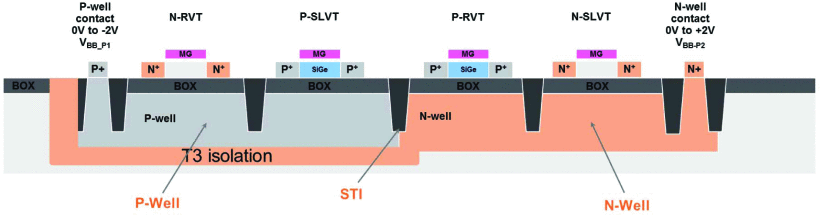
\includegraphics[width=1\textwidth, angle=0]{./figs/theory/wiatr1-p4-wiatr-large}
			    \caption{22FDX cross-sectional construction of active devices \cite{Wiatr2019}.}
			    \label{fig:22fdx_wells}
			\end{figure}
	
	\subsection{MOSFET Models}

	\subsubsection{I-V relations}
	Basic models that describe the large signal current-voltage relations of a Metal Oxide Semiconductor Field Effect Transistor (MOSFET) are introduced here, based wholy from \cite{razavi_2017}. For the purposes of this work, a MOSFET is schematically represented in the manner of figure \ref{fig:mos_symbols}, with gate (G), drain (D), source (S) and backgate (B) terminals. Several operating regimes occur depending on the relation of the terminal voltages. Relevant to the scope of this work, are the linear, saturated and velocity saturated regions of MOSFET operation. Nominally, it is expected that when configured as in figure \ref{fig:vgs_sweep}, sweeping the gate-source voltage ($V_{GS}$), with the drain-source voltage ($V_{DS}$) set greater than 0 in the case of a NFET, that an increasing amount of current will enter the MOSFET drain after crossing a threshold voltage ($V_{TH}$). $V_{TH}$ is predominantly dependent of physical configuration of a FET (dimensions, doping, material), however is impacted by the backgate bias in what is termed "the body effect". A more detailed description of each operating regime will be given in the following discourse.

			\begin{figure}[htb!]
			        \centering
			        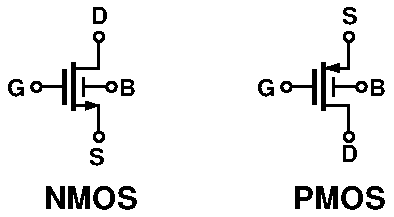
\includegraphics[width=0.5\textwidth, angle=0]{./figs/theory/fet_symbols}
			    \caption{MOSFET symbols.}
			    \label{fig:mos_symbols}
			\end{figure}

			\begin{figure}[htb!]
			        \centering
			        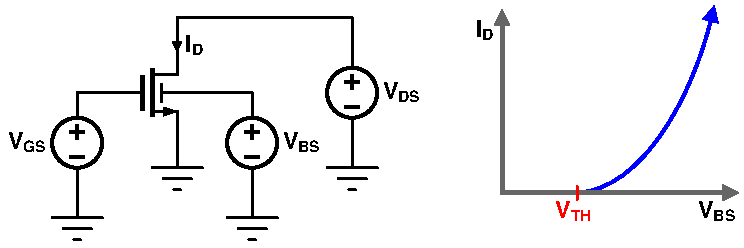
\includegraphics[width=0.8\textwidth, angle=0]{./figs/theory/vgs_sweep}
			    \caption{Drain current versus gate-source bias.}
			    \label{fig:vgs_sweep}
			\end{figure}


	% \textbf{Subthreshold Region}
	% $\xi$ is a factor of ideality, $V_T = k_B T/q$, where $k_B$ is the Boltzmann constant, T is the temperature in Kelvin, and $q$ represents the elementary charge.
	% \begin{equation}
	% 	I_D = I_0e^{\frac{V_{GS}}{\xi V_T}}
	% \end{equation}

	\textbf{Linear Region}
	Linear MOSFET operation occurs under the circumstances where  $|V_{GS}-V_{TH}| > |V_{DS}|$. The following equation is the I-V relation in this regime, where $\mu_n$ represents the electron mobility of the semiconductor in use (within the FET channel), $C_{ox}$ represents the MOS oxide capacitance. 
	\begin{equation}
		I_D = \mu_x C_{ox} \left(\frac{W}{L}\right)\left[(V_{GS}-V_{TH})V_{DS}-\frac{1}{2}V_{DS}^2\right]
	\end{equation}

	\textbf{Saturation Region}
	Saturation region occurs when $|V_{DS}| > |V_{GS}-V_{TH}|$. Notably, dependence of drain current on $V_{DS}$ is reduced, and in the case of the ideal models considered here the effect of $V_{DS}$ are completely negated.
	\begin{equation}
		I_D = \frac{1}{2}\mu_n C_{ox} \left(\frac{W}{L}\right)(V_{GS}-V_{TH})^2
	\end{equation}


	\textbf{Velocity-saturation Region}
	In the scenario of high applied fields which arise in a short MOSFET channels, carrier velocity can saturate to a limited velocity, $v_{sat}$. The point at which this effect takes place is device dependent. For approximate consideration it can be understood to occur when $|V_{DS}/L > E_{crit}|$, where $E_{crit}$ is the electric field which the carrier velocity-electric field relation ($v = \mu E$) of the channel semiconductor becomes sub-linear. Below is the MOSFET model under such circumstances.
	\begin{equation}
		I_D = WC_{ox}(V_{GS}-V_{TH})v_{sat}
	\end{equation}

	\subsubsection{Body Effect}
	Application of a bias to the substrate below a bulk MOSFET, or to the well below a FD-SOI MOSFET has a direct effect on the threshold voltage of a MOSFET. For a bulk MOSFET, change of body bias affects the width of source-drain and source-body depletions, which consequently can increase or decrease the magnitude of the channel inversion charge as seen by the gate terminal. This corresponds to a differential in the threshold voltage. The below equation \cite{razavi_2017} quantifies this effect for bulk devices. $\gamma$ is the body effect coefficient, $2\Phi_F$ represents the MOS surface potential. $V_{TH}$ is non-linearly related to the source-body voltage $V_{SB}$.
	\begin{equation}
		V_{TH} = V_{TH0} + \gamma\left( \sqrt{2\Phi_F + V_{SB}} - \sqrt{|2\Phi_F|} \right)
	\end{equation}
	In the case of FD-SOI transistors, the nature of the body effect is modified due to the presence of the BOX. Thus, an approximate derivation for body effect will be provided here. In FD-SOI, the active channel region is thin, and under strong inversion, the entire channel region is depleted of charge. Supposing a channel height Z and doping $N_A$, the total inversion charge (i.e. to deplete the channel) is $Q_{d} = N_AZ$. With oxide capacitance $C_{ox,fg}$ associated with the front gate, the portion of the threshold voltage associated with total depletion of the channel is, from the front gate perspective:
	\begin{equation}
		V_{d,fg} = \frac{Q_d}{C_{ox,fg}} = \frac{N_AZ}{C_{ox,fg}} 
	\end{equation}
	Supposing that the back gate has capacitance of $C_{ox,bg}$, with bias applied $V_{BS}$, the back gate can be seen to "rob" the front gate of $Q_{bg} = C_{ox,bg}V_{BS}$ when in inversion. Thus results in a partial change of the front gate referred voltage required to obtain channel depletion:
	\begin{equation}
		V_{d,fg}^{'} = \frac{Q_d-Q_{bg}}{C_{ox,fg}} = \frac{Q_d}{C_{ox,fg}} - \frac{C_{ox,bg}}{C_{ox,fg}}V_{BS} = V_{d,fg}-\Delta V_{th,bg}
	\end{equation}
	It is noted that this can be writen as the nominal value of $V_{d,fg}$ minus a differential. This differential is the resulting change in threshold voltage due to back gate bias, $\Delta V_{th,bg}$:
	\begin{equation}
		\Delta V_{th,bg}= \frac{C_{ox,bg}}{C_{ox,fg}}V_{BS} 
	\end{equation}	
	This is linear with applied back gate bias, and that the strength of the coupling is tunable by the ratio of front gate and back gate capacitances. Typically this ration is $<<1$. If we define the body effect coefficient $\gamma$ as:
	\begin{equation}
		\gamma = \frac{C_{ox,bg}}{C_{ox,fg}}
	\end{equation}
	Given a nominal threshold voltage of $V_{TH0}$, in FD-SOI, the threshold voltage can be calculated as:
	\begin{equation}
		V_{TH} = V_{TH0} - \gamma V_{BS}
	\end{equation}


	\subsection{Basic PLL}
	A phase locked loop (PLL) is a feedback system whose output tracks or maintains a fixed phase relationship to an input signal. PLLs are well suited for frequency synthesis, which is the process of generating derivative frequencies from some reference frequency. Given a reference signal with phase trajectory $\Phi_{ref}$ and output signal with phase $\Phi_{out}$, a PLL can be modeled as in figure \ref{fig:basic_fb} using an elementary feedback system, with feedforward and feedback networks A(s) and B(s). 
	\begin{figure}[htb!]
		\center\fontfamily{\sfdefault}\selectfont
% XCircuit output "basic_feedback.tex" for LaTeX input from basic_feedback.ps
\def\putbox#1#2#3#4{\makebox[0.00000in][l]{\makebox[#1][l]{}\raisebox{\baselineskip}[0.00000in][0.00000in]{\raisebox{#2}[0.00000in][0.00000in]{\scalebox{#3}{#4}}}}}
\def\rightbox#1{\makebox[0.00000in][r]{#1}}
\def\centbox#1{\makebox[0.00000in]{#1}}
\def\topbox#1{\raisebox{-0.60\baselineskip}[0.00000in][0.00000in]{#1}}
\def\midbox#1{\raisebox{-0.20\baselineskip}[0.00000in][0.00000in]{#1}}
   \scalebox{1}{
   \normalsize
   \parbox{3.61667in}{
   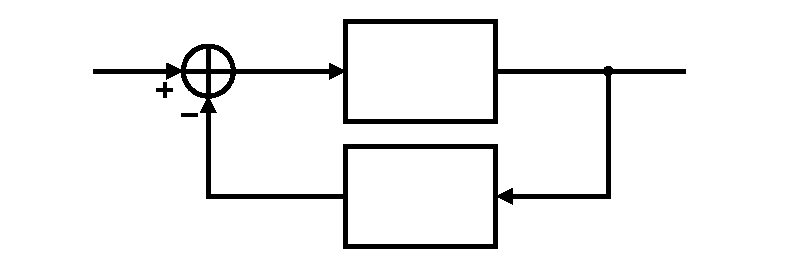
\includegraphics[scale=0.70000]{./figs/basic_feedback.pdf}\\
   % translate x=544 y=496 scale 0.38
   \putbox{1.82000in}{0.85400in}{1.20}{A(s)}%
   \putbox{1.82000in}{0.27300in}{1.20}{B(s)}%
   \putbox{0.44800in}{1.00100in}{1.20}{$\Phi_{ref}$}%
   \putbox{2.84200in}{1.00100in}{1.20}{$\Phi_{out}$}%
   \putbox{1.12000in}{1.00100in}{1.20}{$\Phi_{error}$}%
   } % close 'parbox'
   } % close 'scalebox'
   \vspace{-\baselineskip} % this is not necessary, but looks better
\fontfamily{\rmdefault}\selectfont

		\caption{Phase locked loop as elementary feedback system.}
		\label{fig:basic_fb}
	\end{figure}
	\FloatBarrier
	The closed loop phase response for $\Phi_{ref}$ to $\Phi_{out}$ is therefore:
	\begin{equation}
		\frac{\Phi_{out}(s)}{\Phi_{ref}(s)} = \frac{A(s)}{1+A(s)B(s)}
	\end{equation}
	A case of interest is when B(s) = 1/N, where N is a constant, and the loop gain L(s) = A(s)B(s) $>>$ 1. The closed loop response for this case is:
	\begin{equation}\label{mult_by_n}
		\frac{\Phi_{out}(s)}{\Phi_{ref}(s)} \approx \frac{A(s)}{A(s)B(s)} = \frac{1}{B(s)} = N
	\end{equation}
	We see that the phase through the PLL is multiplied by a factor of N. If the input phase signal is sinusoidal with frequency $\omega_{ref}$, and likewise the output with $\omega_{out}$, then $\phi_{ref}(t)=\omega_{ref}t$ and $\phi_{out}(t)=\omega_{out}t$. Accordingly:
	\begin{equation}
		\frac{\Phi_{out}(t)}{\Phi_{ref}(t)} = \frac{\omega_{out}t}{\omega_{ref}t} \approx N \hspace{1em} \rightarrow \hspace{1em} \omega_{out} \approx N\omega_{ref}
	\end{equation}
	Therefore, it is observed that a PLL allows for the generation of a new frequency from a reference frequency signal, which is termed as "frequency synthesis". With a feedback division ratio of 1/N, the PLL multiplies the reference frequency by a factor of N. Hereon, the B(s) portion of a PLL feedback network is referred to as a divider, with associated division raito N.

	\subsection{PLL Synthesizer Architecture}
		A typical architecture for implementing a physically realizable PLL frequency synthesizer \cite{Razavi1996DesignOM} is shown in figure \ref{fig:basic_pll}. This PLL is comprised of four components: (1) a phase detector, herein PD, (2) a loop filter, herein H$_{LF}$(s), (3) a voltage controlled oscillator, herein VCO, and (4) a divider, indicated as "$\div$ N" in figure \ref{fig:basic_pll}. In control systems parlance, the loop filter corresponds to a controller, the VCO an actuator, and the divider as feedback.
		\begin{figure}[htb!]
			\center\fontfamily{\sfdefault}\selectfont
% XCircuit output "basic_pll.tex" for LaTeX input from basic_pll.ps
\def\putbox#1#2#3#4{\makebox[0.00000in][l]{\makebox[#1][l]{}\raisebox{\baselineskip}[0.00000in][0.00000in]{\raisebox{#2}[0.00000in][0.00000in]{\scalebox{#3}{#4}}}}}
\def\rightbox#1{\makebox[0.00000in][r]{#1}}
\def\centbox#1{\makebox[0.00000in]{#1}}
\def\topbox#1{\raisebox{-0.60\baselineskip}[0.00000in][0.00000in]{#1}}
\def\midbox#1{\raisebox{-0.20\baselineskip}[0.00000in][0.00000in]{#1}}
   \scalebox{1}{
   \normalsize
   \parbox{4.66667in}{
   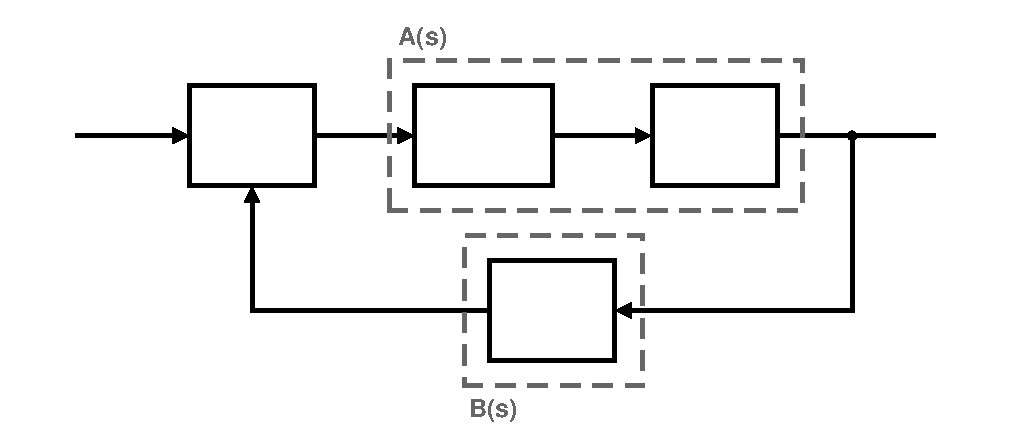
\includegraphics[scale=0.70000]{./figs/basic_pll.pdf}\\
   % translate x=344 y=640 scale 0.38
   \putbox{1.05700in}{1.37900in}{1.20}{PD}%
   \putbox{2.42900in}{0.56700in}{1.20}{$\div$ N}%
   \putbox{0.42000in}{1.52600in}{1.20}{$\Phi_{ref}$}%
   \putbox{3.80100in}{1.52600in}{1.20}{$\Phi_{out}$}%
   \putbox{1.99500in}{1.37900in}{1.20}{H$_{LF}$(s)}%
   \putbox{3.15700in}{1.37900in}{1.20}{VCO}%
   \putbox{1.58200in}{0.70700in}{1.20}{$\Phi_{div}$}%
   \putbox{1.56800in}{1.52600in}{1.20}{$\Phi_e$}%
   \putbox{2.63200in}{1.52600in}{1.20}{V$_{ctrl}$}%
   } % close 'parbox'
   } % close 'scalebox'
   \vspace{-\baselineskip} % this is not necessary, but looks better
\fontfamily{\rmdefault}\selectfont

			\caption{High-level PLL Synthesizer Architecture.}
			\label{fig:basic_pll}
		\end{figure}
		\FloatBarrier
		Further explaination of these components will be hereafter made.

		\subsubsection{Phase Detector}
		A phase detector acts as the summation point of figure \ref{fig:basic_fb}, which measures the phase error $\Phi_e$ between the reference signal and the output of the PLL. The phase error then is then used by the controller, which is implemented as the loop filter. Such a phase detector may also have intrinsic gain, given by $K_{PD}$.
		\begin{equation}
			\Phi_e(s) = K_{PD}(\Phi_{ref}(s) - \Phi_{div}(s))
		\end{equation}

		\subsubsection{Bang-bang phase detector}\label{bbpd_theory}
		% First reference : \cite{toifl_1998}

		\begin{figure}[htb!]
		    \centering
		    \begin{subfigure}{0.5\textwidth}
		        \centering
		        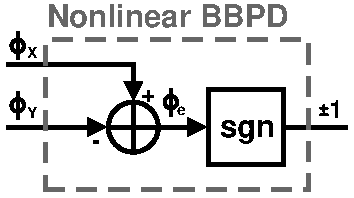
\includegraphics[width=0.75\textwidth, angle=0]{./figs/theory/bbpd_nonlinear}
		        \caption{ }
		        \label{fig:bbpd_nonlinear}
		    \end{subfigure}%
		    \begin{subfigure}{0.5\textwidth}
		        \centering
		        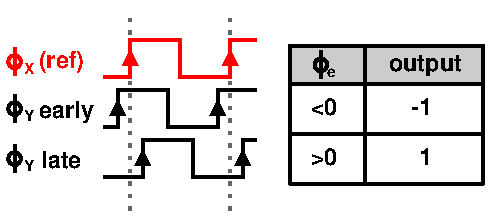
\includegraphics[width=1\textwidth, angle=0]{./figs/theory/bbpd_timing}
		        \caption{ }
		        \label{fig:bbpd_timing}
		    \end{subfigure}
		    % \caption{x.}

		    \caption{\textbf{(a)} BBPD schematic, \textbf{(b)} BBPD timing.}
		    \label{fig:bbpd_theory}
		\end{figure} 
			A simple implementation of a phase detector is a bang-bang phase detector (BBPD) \cite{zanuso_2009}. As exhibited in figure \ref{fig:bbpd_theory}, a BBPD outputs a value of 1 if the input $\Phi_Y$ is late relative to the reference $\Phi_X$ (representing a clock signal), and -1 if it is early. A BBPD shows abrupt nonlinearity in its transfer characteristics. If the error signal variance $\sigma_{\Phi_e}^2$ is constant, which is expected in steady-state PLL operation, a linearized model for phase detector gain can be established \cite{xu_abidi_2017}, given in equation \ref{eq:nom_bbpd_gain}.

			A linearized version of the BBPD is illustrated in figure \ref{fig:bbpd_linearized}. The output $\mathrm{z}$ valued as $\pm 1$ (its variance $\sigma_y^2$=1).
			\begin{equation}\label{eq:nom_bbpd_gain}
				K_{BBPD} = \frac{\mathbb{E}[\Phi_e(t)\cdot\mathrm{z}(t)]}{\mathbb{E}[\Phi_e^2(t)]} = \sqrt{\frac{2}{\pi}}\frac{1}{\sigma_{\Phi_e}}
			\end{equation}
			\begin{figure}[htb!]
				\center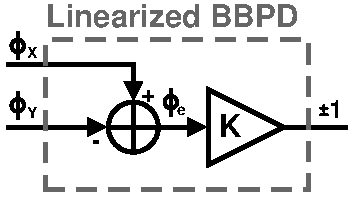
\includegraphics[width=0.4\textwidth, angle=0]{./figs/theory/bbpd_linearized}
				\caption{Linearized bang-bang phase detector.}
				\label{fig:bbpd_linearized}
			\end{figure}

			\subsubsection{BBPD Noise}\label{sec:bbpd_noise}
			Given the output of the BBPD is of fixed power $\sigma_z^2$ = 1, a linearized gain of $K_{BBPD}$, a phase error power of $\mathrm{Var}[\Phi_e(t)] = \sigma_{\Phi_e}^2$, and $\mathbb{E}[\Phi_e(t)]=0$, the noise power  $\sigma_{n_{BBPD}}^2$ out of the BBPD is in equation \ref{eq:bbpd_gain}. $K_{BBPD}^2\sigma_{\Phi_e}^2$ represents the power of the phase error signal component post-detector, and it is assumed that noise power and signal power are uncorrelated.
			\begin{equation}\label{eq:bbpd_gain}
				\sigma_{n_{BBPD}}^2 = \sigma_z^2 - K_{BBPD}^2\sigma_{\Phi_e}^2 = 1-\frac{2}{\pi}
			\end{equation}


			Observe that the BBPD noise power is constant. If the reference signal is a clock signal with frequency $f_{ref}$, the BBPD noise spectral density is in equation \ref{eq:bbpd_noise_psd}.
			\begin{equation}\label{eq:bbpd_noise_psd}
				S_{ n_{BBPD}(f)} = \frac{\sigma_{n_{BBPD}}^2}{\Delta f} = \frac{\left(1-\frac{2}{\pi}\right)}{f_{ref}}
			\end{equation}



		\subsubsection{Divider}
			A divider is used as the feedback path in the PLL, where the division ratio N controls the frequency multiplication of a PLL synthesizer. The transfer function of the divider is:
			\begin{equation}
				\mathrm{H}_{div}(s) = \frac{\Phi_{div}(s)}{\Phi_{out}(s)} = \frac{1}{\mathrm{N}}
			\end{equation}


			Dividers are commonly realized as digital modulo-N counters that count oscillation cycles \cite{weste_harris_2011}. With a division ratio of N, the output of the divider will have an active edge transition (considered to be rising edge as shown in figure \ref{fig:digital_div}) every N input cycles. Phase information is inferred from the output edge timing, which occurs with time interval N$/f_{osc}$, and is equal to the point at which output phase equals a multiple of $2\pi$. Thus a digital divider does not provider continuous phase information, but rather a sampled phase signal with rate $f_{osc}/$N. 
			\begin{figure}[htb!]
				\center\fontfamily{\sfdefault}\selectfont
% XCircuit output "digital_div.tex" for LaTeX input from digital_div.ps
\def\putbox#1#2#3#4{\makebox[0.00000in][l]{\makebox[#1][l]{}\raisebox{\baselineskip}[0.00000in][0.00000in]{\raisebox{#2}[0.00000in][0.00000in]{\scalebox{#3}{#4}}}}}
\def\rightbox#1{\makebox[0.00000in][r]{#1}}
\def\centbox#1{\makebox[0.00000in]{#1}}
\def\topbox#1{\raisebox{-0.60\baselineskip}[0.00000in][0.00000in]{#1}}
\def\midbox#1{\raisebox{-0.20\baselineskip}[0.00000in][0.00000in]{#1}}
   \scalebox{1}{
   \normalsize
   \parbox{3.15000in}{
   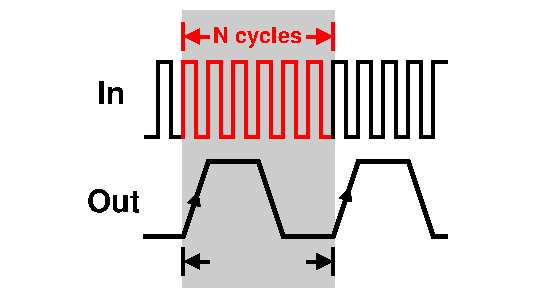
\includegraphics[scale=0.90000]{./figs/digital_div.pdf}\\
   % translate x=-16 y=516 scale 0.38
   \putbox{1.30500in}{0.16200in}{1.20}{$\mathrm{N}/f_{osc}$}%
   } % close 'parbox'
   } % close 'scalebox'
   \vspace{-\baselineskip} % this is not necessary, but looks better
\fontfamily{\rmdefault}\selectfont

				\caption{Digital divider signals.}
				\label{fig:digital_div}
			\end{figure}


		\subsubsection{Loop Filter}
			A loop filter behaves as the controller of a PLL, namely controlling the phase-frequency response of PLL. The choice of loop filter transfer function significatly affects transient PLL behavior, as well as phase noise performance, as is later described. Here, a pole-zero based controller is defined for use in this work. This is designed to have P poles and Z zeros, and can be represented in the canonical form of equation \ref{eq:lf_general_form} as a rational function of polynomials of s with coefficients given with $\{a_0, ..., a_P\}$ and $\{b_0, ..., b_Z\}$.
			\begin{equation} \label{eq:lf_general_form}
				\textnormal{H}_{LF}(s) = \frac{\sum_{j=0}^Z b_js^j}{\sum_{k=0}^P a_ks^k}
			\end{equation}
			
		\subsubsection{Loop Filter Discretization and Digitization}\label{lf-discretization}
			In PLLs which sample on a fixed interval, defined by a reference clock frequency $f_{ref}$, derivation of a discrete time controller model is necessary. This is derived from the continuous canonical loop filter (equation \ref{eq:lf_general_form}) via application of a continous s-domain to discrete z-domain transformation. Strictly speaking, $z^{-1} = e^{-s\Delta T_s}$ for values on the unit circle, i.e. r=1 \cite{proakis_1993_z}. However, if the PLL sampling rate $f_s$=$f_{ref}$ is constrained to be sufficiently higher than the implemented filter bandwidth (i.e. PLL loop bandwidth, $BW_{loop}$), a simpler transformation using a truncated Taylor series approximation is applicable. Given the $1/\Delta T_s$=$f_{s}$ as the relation for sampling rate, then:
			\begin{align*}
				z^{-1} &= e^{-s\Delta T_s} && \text{(definition of z on unit circle)} \\
				&= \sum_{k=0}^\infty\frac{(-s\Delta T_s)^k}{k!} && \text{(exponential Taylor series)} \\
				&\approx 1-s\Delta T_s &&\text{(if $|s\Delta T_s| = 2\pi\mathrm{BW}_{loop}\cdot \Delta T_s << 1$)} \\
			\end{align*}
			Thus the s-to-z and z-to-s identities for the approximate transform are:
			\begin{align}
				z^{-1} &= 1-s\Delta T_s\\
				s &= \frac{1}{\Delta T_s}(1-z^{-1}) \label{eq:s_to_z_xfrm}
			\end{align}
			Applying equation \ref{eq:s_to_z_xfrm} to the general loop filter of equation \ref{eq:lf_general_form} yields the z-domain loop filter:
			\begin{align}
				\textnormal{H}_{LF}(z) &= \left.\textnormal{H}_{LF}(s)\right\vert_{s=\frac{1}{\Delta T_s}(1-z^{-1})} = \left.\frac{\sum_{j=0}^Z b_js^j}{\sum_{k=0}^P a_ks^k}\right\vert_{s=\frac{1}{\Delta T_s}(1-z^{-1})}\\
				&= \frac{\sum_{j=0}^Z \frac{b_j}{\Delta T_s^j}(1-z^{-1})^j}{\sum_{k=0}^P \frac{a_k}{\Delta T_k}(1-z^{-1})^k} \label{eq:z_general_lf}
			\end{align}
			Equation \ref{eq:z_general_lf} is transformed into a digitally implementable form by reorganizing into the canonical representation of equation \ref{eq:canonical_z_tf}, which then determines the tap coefficients for the sampled-time difference equation in equation \ref{eq:cananical_diff_eq}. 
			\begin{align}
				\textnormal{H}_{LF}(z) &= \frac{\sum_{j=0}^P b_j^{'}z^{-j}}{1+\sum_{k=1}^Z a_k^{'}z^{-k}}\label{eq:canonical_z_tf} \\
				y[n]&= -\sum_{k=1}^P a_k^{'}y[n-k] + \sum_{j=0}^Z b_j^{'}x[n-j] \label{eq:cananical_diff_eq}
			\end{align}
			The obtained difference equation is directly implementable in digital hardware with a direct form-I IIR filter \cite{proakis_1993} shown in figure \ref{fig:filt_implementation}. Such a design is a cantidate for automatic synthesis of digital logic. The filter coefficients $\{a_1^{'}, ..., a_P^{'}\}$ and $\{b_0^{'}, ..., b_Z^{'}\}$ must be quantized into finite resolution fixed point words for a complete digital implementation. The delay elements ($z^{-1}$ blocks) are implementable digitally as registers, the coefficient gains are implementable with array multipliers, and the adders are implementable with digital adders.
			\begin{figure}[htb!]
				\center\fontfamily{\sfdefault}\selectfont
% XCircuit output "direct_type_1_primed.tex" for LaTeX input from direct_type_1_primed.ps
\def\putbox#1#2#3#4{\makebox[0.00000in][l]{\makebox[#1][l]{}\raisebox{\baselineskip}[0.00000in][0.00000in]{\raisebox{#2}[0.00000in][0.00000in]{\scalebox{#3}{#4}}}}}
\def\rightbox#1{\makebox[0.00000in][r]{#1}}
\def\centbox#1{\makebox[0.00000in]{#1}}
\def\topbox#1{\raisebox{-0.60\baselineskip}[0.00000in][0.00000in]{#1}}
\def\midbox#1{\raisebox{-0.20\baselineskip}[0.00000in][0.00000in]{#1}}
   \scalebox{1}{
   \normalsize
   \parbox{2.75990in}{
   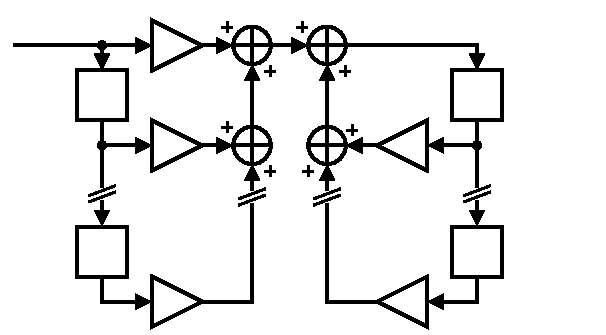
\includegraphics[scale=0.70000]{./figs/direct_type_1_primed.pdf}\\
   % translate x=936 y=992 scale 0.38
   \putbox{0.04200in}{1.42800in}{0.96}{x[n]}%
   \putbox{2.28200in}{1.33700in}{0.96}{y[n]}%
   \putbox{0.37800in}{1.07800in}{0.96}{$z^{-1}$}%
   \putbox{0.84000in}{1.45600in}{0.96}{b$_0^{'}$}%
   \putbox{0.84000in}{0.98700in}{0.96}{b$_1^{'}$}%
   \putbox{2.12800in}{1.07800in}{0.96}{$z^{-1}$}%
   \putbox{2.12800in}{0.34300in}{0.96}{$z^{-1}$}%
   \putbox{1.71500in}{1.00100in}{0.96}{-a$_1^{'}$}%
   \putbox{1.70100in}{0.27300in}{0.96}{-a$_\mathrm{P}^{'}$}%
   \putbox{2.28200in}{0.86800in}{0.96}{y[n-1]}%
   \putbox{0.37800in}{0.34300in}{0.96}{$z^{-1}$}%
   \putbox{0.84000in}{0.25900in}{0.96}{b$_\mathrm{Z}^{'}$}%
   } % close 'parbox'
   } % close 'scalebox'
   \vspace{-\baselineskip} % this is not necessary, but looks better
\fontfamily{\rmdefault}\selectfont

				\caption{Direct form I implementation of IIR filter.}
				\label{fig:filt_implementation}
			\end{figure}


			
		\subsubsection{Voltage/Digitally Controlled Oscillator}
			A controlled oscillator is an oscillator with frequency controlled by an input signal. When this input signal takes the form of an analog voltage $\textnormal{V}_{ctrl}$, it is referred to as a voltage controlled oscillator (VCO). Otherwise, when controlled digitally with an oscillator tuning work (OTW) u[n], it is referred to as a digitally controlled oscillator (DCO). Nominally, a controlled oscillator is characterized by its gain, in the case of a VCO is $K_{VCO} = \partial f/\partial \textnormal{V}_{ctrl}$. With a DCO, the gain is $K_{DCO} = \Delta f/LSB$, that is the change in frequency per least significant bit. Analyzed in terms of phase (for the VCO case), an oscillator can be seen as a time-phase integrator, provided a nominal oscillator frequency of $f_0$:
			\begin{equation}\label{eq:vco_ph}
				\Phi_{VCO}(t) = \Phi_{out}(t) = \int2\pi(K_{VCO}\textnormal{V}_{ctrl}(t) + f_0)\mathrm{dt}
			\end{equation}
			In the s-domain, the transfer function for a VCO is in equation \ref{eq:vco_tf} and equation \ref{eq:dco_tf} for a DCO. 
			\begin{equation}\label{eq:vco_tf}
				\mathrm{H}_{VCO}(s) = \frac{\Phi_{VCO}(s)}{\textnormal{V}_{ctrl}(s)} = \frac{2\pi K_{VCO}}{s}
			\end{equation}
			\begin{equation}\label{eq:dco_tf}
				\mathrm{H}_{DCO}(s) = \frac{\Phi_{VCO}(s)}{\textnormal{u}(s)} =  \frac{2\pi K_{DCO}}{s}
			\end{equation}
			By application of discretization and conversion to difference equations, the sampled-time oscillator phase signals are equation \ref{eq:vco_ph_de} for a VCO and equation \ref{eq:dco_ph_de} for a DCO. 
			\begin{equation}\label{eq:vco_ph_de}
				\Phi_{out}[n] = \Phi_{out}[n-1] + 2\pi K_{VCO}\Delta T_s\textnormal{V}_{ctrl}[n]
			\end{equation}
			\begin{equation}\label{eq:dco_ph_de}
				\Phi_{out}[n] = \Phi_{out}[n-1] + 2\pi K_{DCO}\Delta T_su[n]
			\end{equation}

		\subsubsection{Closed Loop PLL Transfer Function}\label{cont_pll_tf}
			With a PLL described at the component level, the closed loop dynamics of the PLL can be computed. A PLL loop gain L(s) can be first determined (using BBPD definition for phase detector gain). 
			\begin{equation}
				\mathrm{L}(s) = K_{PD}\textnormal{H}_{LF}(s)\textnormal{H}_{DCO}(s)\textnormal{H}_{div}(s) = \frac{2\pi K_{PD}K_{DCO}}{\mathrm{N}}\frac{1}{s}\frac{\sum_{j=0}^Z b_js^j}{\sum_{k=0}^P a_ks^k}
			\end{equation}
			Closing the loop with the phase detector as the feedback summation point, the response of the PLL from reference to output is in equation \ref{eq:cont_pll_tf}.
			\begin{align} \label{eq:cont_pll_tf}
				\mathrm{T}(s) = \frac{\Phi_{out}(s)}{\Phi_{ref}(s)} = \frac{2\pi K_{PD}K_{DCO}\sum_{j=0}^Z b_js^j}{\sum_{k=0}^P a_ks^{k+1} + \frac{2\pi K_{PD}K_{DCO}}{\mathrm{N}}\sum_{j=0}^Z b_js^j} = \mathrm{N}\frac{\mathrm{L}(s)}{1 + \mathrm{L}(s)}
			\end{align}



	%%%%%%%%%%%%%%%%%%%%%%%%%%%%%%%%%%%%%%%%%%%%%%%%%%%%%%%%%%%%%%%%%%%%%%%%%%%%%%%%%%%%%
	\subsection{Phase noise}
		Phase noise can be described as undesired variation in an oscillator's phase trajectory from ideal. If an oscillator's frequency is $\omega_{osc}$, then with additive phase noise, the phase of an oscillator is in \ref{eq:osc_ph_traj}. 
		\begin{equation}\label{eq:osc_ph_traj}
			\Phi_{osc}(t) = \omega_{osc}t + \Phi_n(t)
		\end{equation}
		This is composed of a linear phase component $\omega_{osc}t$ and a noise component $\Phi_n(t)$. In the frequency domain, the effect of phase noise is that it broadens the tone of the oscillator, as shown in figure \ref{fig:phase_noise_psd}. Phase noise can be viewed as instability in terms of oscillator frequency.
		\begin{figure}[htb!]
	        \centering
	        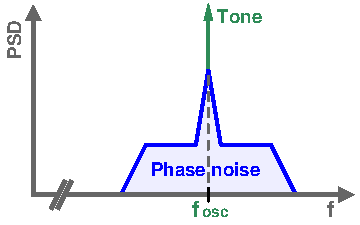
\includegraphics[width=0.5\textwidth, angle=0]{./figs/theory/phase_noise_psd}
		    \caption{Effect of phase noise on frequency tone.}
		    \label{fig:phase_noise_psd}
		\end{figure}

		\subsubsection{Relation to Power spectral density}\label{sec:pn_to_psd}
		An oscillator's voltage waveform can be described in terms of a phase trajectory function $\Phi_{osc}(t)$ and amplitude $A_0$ in the following manner (ignoring higher harmonics):
		\begin{equation}\label{eq:osc_wfm}
			V_{osc}(t) = \Re\left\{A_0e^{j\Phi_{osc}(t)}\right\}
		\end{equation}
		 In an oscillator, it is desirable for phase noise to be small, and zero mean ($\mathbb{E}[\Phi_{n}(t)]=0$). Using a constraint $\mathrm{Var}[\Phi_{n}(t)] << 1$ the following approximations can be applied to determine the oscillators spectral density in terms of the phase noise component $\Phi_n(t)$.
		\begin{align}
			V_{osc}(t) &= \Re\left\{A_0e^{j\omega_{osc}t}e^{j\Phi_{n}(t)}\right\} && \text{(oscillator waveform)} \\
			&= \Re\left\{A_0e^{j\omega_{osc}t}\sum_{k=0}^\infty\frac{(j\Phi_{n}(t))^k}{k!}\right\} && \text{(apply exponential Taylor series)} \\
			&\approx  \Re\left\{A_0e^{j\omega_{osc}t} +j\Phi_{n}(t)A_0e^{j\omega_{osc}t}\right\} && \text{(truncate series at k=1 given $\mathrm{Var}[\Phi_{n}(t)] << 1$)} \\
			&= A_0\cos(\omega_{osc}t) - \Phi_{n}(t)A_0\sin(\omega_{osc}t) &&\text{(taking real component)}\label{eq:pll_out_approx}\\
		\end{align}
		The result is a carrier cosine signal, and an orthogonal sine signal modulated by the phase noise $\Phi_{n}$. From this, the spectral density of the phase noise relative to the carrier can be estimated. The power spectral density $S_{V_{osc}}$ is computed in equations \ref{eq:psd_vout}-\ref{eq:psd_noise}. Due to orthogonality of the sine/cosine components of equation \ref{eq:pll_out_approx}, the cross terms that appear in the PSD computation are zero. 
		\begin{align}
			S_{V_{out}}(f) =& \lim_{\Delta T\rightarrow\infty}\frac{1}{\Delta T}|\mathcal{F}\{V_{out}(t)\cdot\mathrm{rect}(t/\Delta T)\}|^2 \label{eq:psd_vout}\\
			=&\lim_{\Delta T\rightarrow\infty}\frac{A_0^2}{\Delta T}|\mathcal{F}\{\cos(\omega_{osc}t)\cdot\mathrm{rect}(t/\Delta T)\}|^2 \label{eq:psd_carrier}\\ 
			&+ \lim_{\Delta T\rightarrow\infty}\frac{A_0^2}{\Delta T}|\mathcal{F}\{\Phi_{n}(t)\cdot\mathrm{rect}(t/\Delta T)\}*\mathcal{F}\{\sin(\omega_{osc}t)\cdot\mathrm{rect}(t/\Delta T)\}|^2 \label{eq:psd_noise}\\
		\end{align}
		 The noise power spectral density function of the output waveform $\mathcal{L}(\Delta f)$ is defined as the noise PSD at offset $\Delta f$ from the carrier frequency $f_{osc}$, normalized to the carrier power. Here the PSD of the carrier component is given by equation \ref{eq:psd_carrier}, and the noise component by equation \ref{eq:psd_noise}. Shifting equation \ref{eq:psd_noise} by $-\omega_{osc}$ and performing normalization for carrier power results in:
		\begin{equation}\label{eq:pn_psd_relation}
			\mathcal{L}(\Delta f) = \left.\lim_{\Delta T\rightarrow\infty}\frac{1}{\Delta T}|\mathcal{F}\{\Phi_{n}(t)\cdot\mathrm{rect}(t/\Delta T)\}|^2 \right|_{f=\Delta f}= S_{\Phi_{n}}(\Delta f)
		\end{equation}

		Thus, the noise PSD $\mathcal{L}(\Delta f)$ of the PLL output waveform relative to the carrier is equal to the PSD of the phase noise signal $\Phi_{n}(t)$, provided $\text{Var}[\Phi_{n}(t)] << 1$. The PSD of $\Phi_{n}(t)$ is notated as $S_{\Phi_{n}}(\Delta f)$.


	\subsubsection{Leeson's model}\label{dco_noise}
		Oscillator noise from thermal and stochastic sources is typical represented mathematically using Leeson's model for oscillator phase noise \cite{leeson_1966}. Leeson's model considers noise power density at an offset $\Delta f$ from the oscillator tone (carrier). Noise power density is represented with the function $\mathcal{L}(\Delta f)$, which is the noise power density normalized to the power of the oscillator carrier tone, in other words in units of dBc/Hz. Leeson's model divides phase noise into three regions, illustrated in figure \ref{fig:leeson_pn}: (1) flicker-noise dominated, with a slope of -30 dB/decade, (2) white frequency-noise dominated, with -20 dB per decade, and (3) a flat region, limited by the thermal noise floor or amplitude noise. It is noted that phase noise components are at frequencies different than the carrier, hence are orthogonal, and can be treated as independent components that are added to the main oscillator tone signal for analysis. 

			\begin{figure}[htb!]
		        \centering
		        \fontfamily{\sfdefault}\selectfont
% XCircuit output "leeson_pn.tex" for LaTeX input from leeson_pn.ps
\def\putbox#1#2#3#4{\makebox[0.00000in][l]{\makebox[#1][l]{}\raisebox{\baselineskip}[0.00000in][0.00000in]{\raisebox{#2}[0.00000in][0.00000in]{\scalebox{#3}{#4}}}}}
\def\rightbox#1{\makebox[0.00000in][r]{#1}}
\def\centbox#1{\makebox[0.00000in]{#1}}
\def\topbox#1{\raisebox{-0.60\baselineskip}[0.00000in][0.00000in]{#1}}
\def\midbox#1{\raisebox{-0.20\baselineskip}[0.00000in][0.00000in]{#1}}
   \scalebox{1}{
   \normalsize
   \parbox{2.68750in}{
   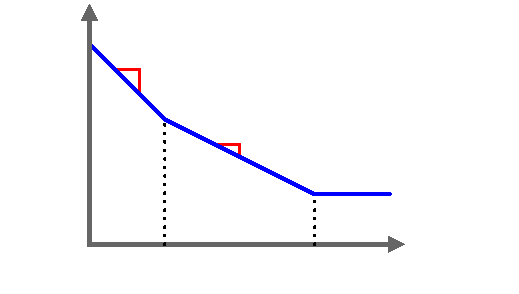
\includegraphics[scale=0.80000]{./figs/leeson_pn.pdf}\\
   % translate x=-248 y=245 scale 0.38
   \putbox{1.88000in}{0.06400in}{0.90}{$\log(\Delta f)$}%
   \putbox{0.80800in}{1.23200in}{0.72}{-30 dB/dec}%
   \putbox{0.80800in}{1.09600in}{0.72}{$\propto f^{-3}$}%
   \putbox{1.34400in}{0.73600in}{0.72}{$\propto f^{-2}$}%
   \putbox{1.34400in}{0.86400in}{0.72}{-20 dB/dec}%
   \putbox{0.80800in}{0.13600in}{0.72}{\rotatebox{-360}{$f_1$}}%
   \putbox{1.60800in}{0.13600in}{0.72}{\rotatebox{-360}{$f_2$}}%
   \putbox{0.04800in}{1.40000in}{0.90}{$\mathcal{L}(\Delta f)$}%
   } % close 'parbox'
   } % close 'scalebox'
   \vspace{-\baselineskip} % this is not necessary, but looks better
\fontfamily{\rmdefault}\selectfont

			    \caption{Phase noise regions of Leeson's model.}
			    \label{fig:leeson_pn}
			\end{figure}

		The equation for $\mathcal{L}(\Delta f)$ (from \cite{lee_hajimiri_2000}) is in equation \ref{eq:leesons}, and is dependent on temperature T, excess noise factor F, oscillator power P, oscillator Q factor, and the transition frequencies $f_1$ and $f_2$ that separate the different noise regions. It is of interest to note that the phase noise relative to the carrier will increase as power decreases, which provides challenge for creating low power oscillators with acceptable phase noise characteristics. 
		\begin{equation}\label{eq:leesons}
		\mathcal{L}(\Delta f) = 10\log_{10}\left[\frac{2\text{F}k_B\text{T}}{\text{P}}\left(1+\left(\frac{f_2}{2Q\Delta f}\right)^2\right)\left(1+\frac{f_1}{|\Delta f|}\right)\right] = S_{\Phi n_{DCO}}(\Delta f)
		\end{equation}
		For notational consistency, the following redefinition is used in the remainder of this paper: $S_{\Phi n_{DCO}}(f) = \mathcal{L}(\Delta f)|_{\Delta f = f}$

	\subsubsection{Phase Noise Figures of Merit}
	A common method to assign a figure of merit (FOM) to oscillator phase noise performance is to utilize the below relation \cite{Kinget1999}. Such a model assumes linear tradeoffs between power, frequency, and phase noise, and assumes that the rolloff of phase noise will occur with -20 dB/decade. A Lower FOM here is better.
	\begin{equation}\label{eq:fom_pn}
		\textnormal{FOM}_{\textnormal{pn}} = 10\log_{10}\left(\frac{\textnormal{Power}}{\textnormal{1 mW}}\cdot\left(\frac{\Delta f}{f_0}\right)^2\right) + \mathcal{L}(\Delta f)
	\end{equation}
	Another FOM applied to PLLs is provided below, based on the RMS jitter of the PLL \cite{XiangGao2009}. Here, RMS jitter is used as the phase spectrum of a PLL is often more complicated than a simple oscillator, containing spurs, in-band phase noise supression, and peaking resulting from the PLL loop filter. It should be noted that RMS jitter (in time) is tied directly to total phase noise power, as expected by Parseval's theorem \cite{parseval_1799}.  Lower is better again with this FOM. 
	\begin{equation}\label{eq:fom_jitter}
		\textnormal{FOM}_{\textnormal{jitter}} = 10\log_{10}\left(\frac{\sigma_{t_j}^2}{(\textnormal{1 s})^2}\cdot\frac{\textnormal{Power}}{\textnormal{1 mW}}\right)
	\end{equation}
	\begin{equation}
		\sigma_{t_j}^2 = \frac{\mathrm{Var}[\Phi_{n}(t)]}{\omega_0^2}
	\end{equation}
	In general, a good figure of merit is arrived to be decreasing power and/or minimizing total phase noise power. 
	
	\subsubsection{Ring Oscillator Phase Noise}
	Oscillator phase noise for ring oscillators has a well defined limit as determined by analysis of noise of ideal RC circuits \cite{Navid2005}, which is provided in equation \ref{eq:ro_pn}. Note that his model is limited to analyzing the-20 dB/decade part of an oscillator's spectrum as seen by Leeson's model.
	\begin{equation}\label{eq:ro_pn}
		\mathcal{L}_{min}(\Delta f)= 10\log 10\left(\frac{7.33k_BT}{P}\left(\frac{f_0}{\Delta f}\right)^2\right)
	\end{equation}
	Applying this to the phase noise FOM equation \ref{eq:fom_pn}, a limit for ring oscillator phase noise FOM is determined in equation \ref{eq:ro_fom_limit}.
	\begin{equation}\label{eq:ro_fom_limit}
		\textnormal{FOM}_{\textnormal{jitter}}(T) = 10\log 10\left(7330k_BT\right)
	\end{equation}
	At 300K, it is then expected that the jitter FOM for a ring oscillator should approach -165.2 dB. An example state of art comparison figure in \ref{fig:lc_ro_fom} shows clustering by oscillator type of jitter FOM calculated in various published works in \cite{Tohidian2015}. It is seen the FOM value calculated from theory is close to that seen implemented hardware.
	\begin{figure}[htb!]
		\center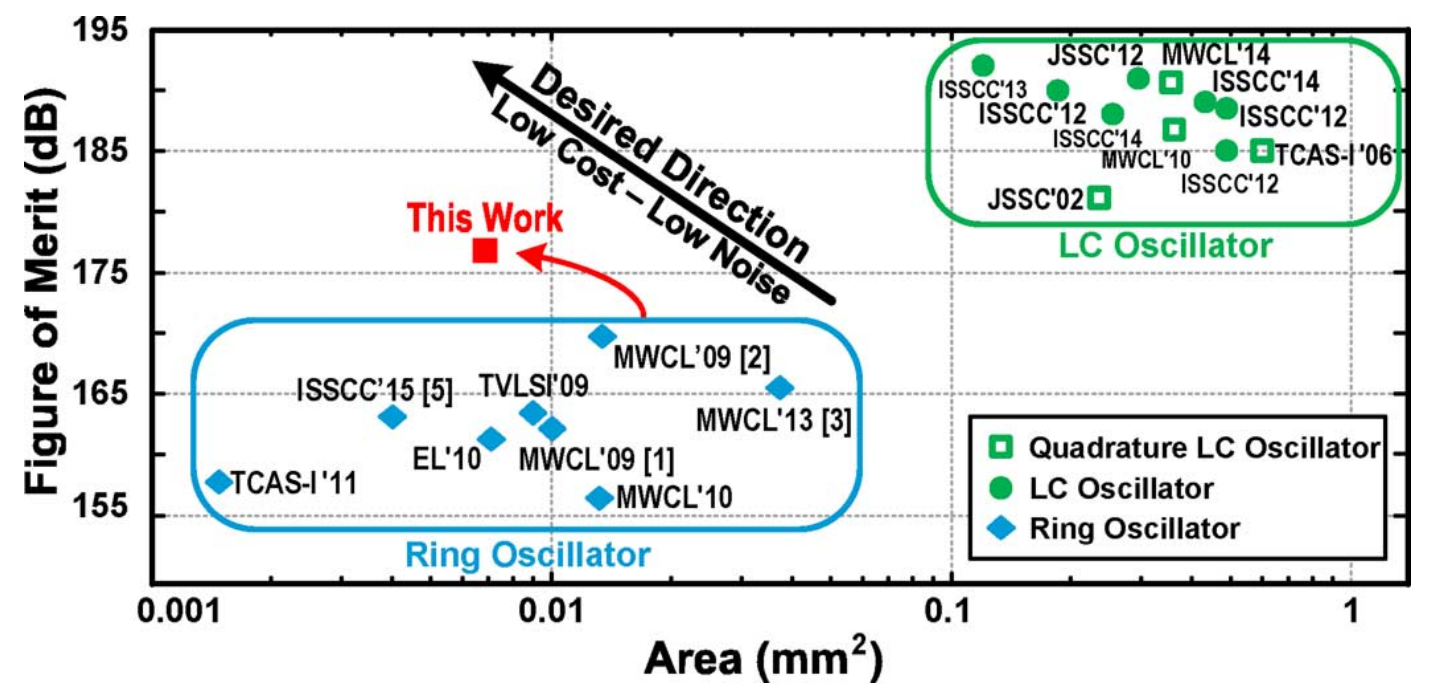
\includegraphics[width=1\textwidth, angle=0]{./figs/lc_ro_fom_comparison}
		\caption{FOM$_{jitter}$ of various LC and ring oscillators \cite{Tohidian2015}.}
		\label{fig:lc_ro_fom}
	\end{figure}

	\FloatBarrier



\subsection{PLL Phase Noise}\label{ntfs}
	Having an understanding of PLL theory, individual PLL component characteristics, and phase noise, a model for PLL phase noise can be constructed. To begin, noise sensitivity transfer functions are defined to refer each noise source to the PLL output. Here, all noise sources have been defined as additive signal components to each PLL component output. The full system noise model is in figure \ref{fig:full_pll_noise}.
	\begin{figure}[htb!]
		\center\fontfamily{\sfdefault}\selectfont
% XCircuit output "discrete_pll_full_noise.tex" for LaTeX input from discrete_pll_full_noise.ps
\def\putbox#1#2#3#4{\makebox[0.00000in][l]{\makebox[#1][l]{}\raisebox{\baselineskip}[0.00000in][0.00000in]{\raisebox{#2}[0.00000in][0.00000in]{\scalebox{#3}{#4}}}}}
\def\rightbox#1{\makebox[0.00000in][r]{#1}}
\def\centbox#1{\makebox[0.00000in]{#1}}
\def\topbox#1{\raisebox{-0.60\baselineskip}[0.00000in][0.00000in]{#1}}
\def\midbox#1{\raisebox{-0.20\baselineskip}[0.00000in][0.00000in]{#1}}
   \scalebox{1}{
   \normalsize
   \parbox{6.30000in}{
   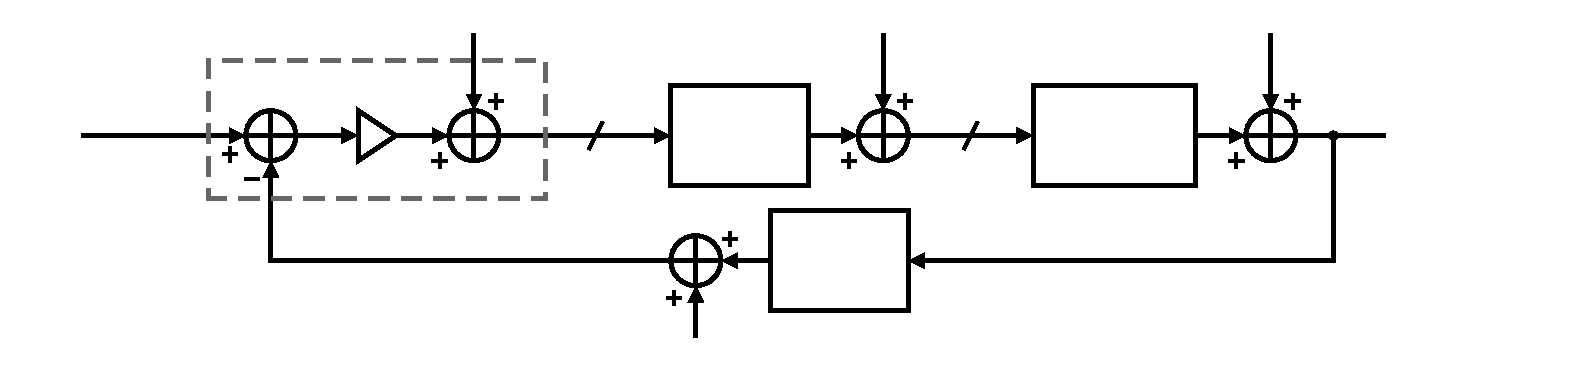
\includegraphics[scale=0.60000]{./figs/discrete_pll_full_noise.pdf}\\
   % translate x=416 y=544 scale 0.38
   \putbox{0.33600in}{1.00800in}{0.84}{$\Phi_{ref}$(t)}%
   \putbox{1.56000in}{0.51000in}{0.84}{$\Phi_{div}$(t)}%
   \putbox{2.27400in}{1.03200in}{0.84}{e$_\Phi$(t)}%
   \putbox{1.42200in}{1.08600in}{0.84}{\rotatebox{-360}{$K_{PD}$}}%
   \putbox{1.20600in}{1.00800in}{0.84}{$\Phi_e$}%
   \putbox{0.83400in}{1.28400in}{0.84}{PD}%
   \putbox{2.77200in}{0.89400in}{0.84}{H$_{LF}$(s)}%
   \putbox{3.79800in}{1.02000in}{0.84}{u(t)}%
   \putbox{4.26000in}{0.90600in}{0.84}{$\frac{2\pi K_{DCO}}{s}$}%
   \putbox{5.22000in}{0.99600in}{0.84}{$\Phi_{out}$(t)}%
   \putbox{3.22200in}{0.39600in}{0.84}{$\div$ N}%
   \putbox{4.13400in}{1.17000in}{0.84}{DCO}%
   \putbox{1.93200in}{1.30800in}{0.84}{q$_{n_{PD}}$(t)}%
   \putbox{3.57000in}{1.30800in}{0.84}{\rotatebox{-360}{q$_{n_{LF}}$(t)}}%
   \putbox{2.82000in}{0.09600in}{0.84}{$\Phi_{n_{div}}$(t)}%
   \putbox{5.12400in}{1.30800in}{0.84}{$\Phi_{n_{DCO}}$(t)}%
   } % close 'parbox'
   } % close 'scalebox'
   \vspace{-\baselineskip} % this is not necessary, but looks better
\fontfamily{\rmdefault}\selectfont

		\caption{Full PLL additive noise model.}
		\label{fig:full_pll_noise}
	\end{figure}
	\FloatBarrier
	\subsubsection{PLL Noise Transfer Functions}
	Following the approach of \cite{perrott_2002}, a transfer function $\hat{\mathrm{T}}(s)$ is defined in equation \ref{eq:parameterizing_tf} which characterizes the normalized closed loop phase response from reference input to output of the PLL. $L(s)$ is the PLL loop gain and $T(s)$ is the PLL closed loop transfer function. 
	\begin{equation}\label{eq:parameterizing_tf}
	\hat{\mathrm{T}}(s) = \frac{\mathrm{L}(s)}{1+\mathrm{L}(s)}\hspace{1em} \text{s.t.} \hspace{1em} \mathrm{T}(s) = \frac{\Phi_{out}}{\Phi_{ref}} = \mathrm{N}\hat{\mathrm{T}}(s) 
	\end{equation}
	Solving for the closed transfer functions between each noise source ($q_{n_{BBPD}}$, $q_{n_{LF}}$, $\Phi_{n_{DCO}}$ and $\Phi_{n_{div}}$) to the output $\Phi_{out}$ in the s-domain yields equations \ref{eq:noise_tf_tdc}-\ref{eq:noise_tf_div}.
	\begin{align}
		\frac{\Phi_{out}(s)}{q_{n_{PD}}(s)} & = \frac{2\pi\frac{K_{DCO}}{s}\mathrm{H}_{LF}(s)}{1+\mathrm{L}(s)}= \frac{\mathrm{N}}{\mathrm{K_{PD}}}\frac{\mathrm{L}(s)}{1+\mathrm{L}(s)} = \frac{\mathrm{N}}{\mathrm{K_{PD}}}\hat{\mathrm{T}}(s)\label{eq:noise_tf_tdc}\\
		\frac{\Phi_{out}(s)}{\Phi_{n_{DCO}}(s)} & = \frac{1}{1+\mathrm{L}(s)}= 1-\hat{\mathrm{T}}(s)\\
		\frac{\Phi_{out}(s)}{q_{n_{LF}}(s)} & = \frac{2\pi\frac{K_{DCO}}{s}}{1+\mathrm{L}(s)} = 2\pi\frac{K_{DCO}}{s}(1-\hat{\mathrm{T}}(s))\\
		\frac{\Phi_{out}(s)}{\Phi_{n_{div}}(s)} & =\frac{K_{BBPD} 2\pi \frac{K_{DCO}}{s}\mathrm{H}_{LF}(s)}{1+\mathrm{L}(s)}= \mathrm{N}\frac{\mathrm{L}(s)}{1+\mathrm{L}(s)} = \mathrm{N}\hat{\mathrm{T}}(s)\label{eq:noise_tf_div}
	\end{align}

	\subsubsection{PLL Output-referred Noise}\label{sec:pll_output_noise}
		Using the noise transfer functions, the expressions for noise power spectrum of the BBPD (equation \ref{eq:bbpd_noise_psd}) and the noise spectrum of a ring oscillator (equation \ref{eq:ro_pn}), the PLL output phase noise spectrum of each component is determined by multiply the respective noise transfer function with the respective noise spectral density. Here it is found that the BBPD noise component out of the PLL is given in equation \ref{eq:out_psd_bbpd_pll}, and the oscillator component is given in equation \ref{eq:out_psd_dco_pll}. The loop filter and divider components are here ignored, as they will be shown not be relevant in this work. 

		% \begin{equation}\label{eq:bbpd_noise_psd}
		% 	S_{ n_{BBPD}(f)} = \frac{\sigma_{n_{BBPD}}^2}{\Delta f} = \frac{\left(1-\frac{2}{\pi}\right)}{f_{ref}}
		% \end{equation}
			% \begin{align}\label{eq:cl_bbpd_pll}
			% 	\mathrm{T}(s)=\frac{\Phi_{out}(s)}{\Phi_{ref}(s)} = \frac{2\pi \sqrt{\frac{2}{\pi}}\frac{1}{\sigma_{\Phi_e}}K_{DCO}\sum_{j=0}^Z b_js^j}{\sum_{k=0}^P a_ks^{k+1} + 2\pi \sqrt{\frac{2}{\pi}}\frac{\mathrm{1}}{\sigma_{\Phi_e}\mathrm{N}}K_{DCO}\sum_{j=0}^Z b_js^j} = \mathrm{N}\frac{\mathrm{L}(s)}{1+\mathrm{L}(s)}
			% \end{align}
		% \begin{align}\label{eq:ntf_bbpd_pll}
		% 	\frac{\Phi_{out}(f)}{q_{n_{{BBPD}}}(f)} = \sqrt{\frac{\pi}{2}}\sigma_{\Phi_e}\mathrm{N}\frac{\mathrm{L}(f)}{1+\mathrm{L}(f)} = \sqrt{\frac{\pi}{2}}\sigma_{\Phi_e}\mathrm{N}\hat{\mathrm{T}}(f)
		% \end{align}
		\begin{align}\label{eq:out_psd_bbpd_pll}
			S_{\Phi n_{BBPD,out}}(f) &= S_{n_{BBPD}}(f)\left|\frac{\Phi_{out}(f)}{q_{n_{BBPD}}(f)}\right|^2 = \frac{\left(\frac{\pi}{2}-1\right)}{f_{ref}}\left|\sigma_{\Phi_e}\mathrm{N}\hat{\mathrm{T}}(f)\right|^2
		\end{align}
		\begin{align}\label{eq:out_psd_dco_pll}
			S_{\Phi n_{DCO,out}}(f) &= \mathcal{L}_{min}(f)\left|\frac{\Phi_{out}(f)}{q_{n_{DCO}}(f)}\right|^2 = \frac{7.33k_BT}{P}\left(\frac{f_0}{\Delta f}\right)^2|1-\hat{\textnormal{T}}(\Delta f)|^2 
		\end{align}
		The total output noise power spectral density is given as the sum of the components, presuming independence of all noise sources. Following the results of section \ref{sec:pn_to_psd}, which determined that oscillator power spectrum is equivalent to the phase noise power spectrum for zero mean phase noise with low power, the final oscillator power spectrum at $\Delta f$ from the carrier is in equation \ref{eq:pll_noise_psd}.
		\begin{align}
			S_{n_{PLL}}(f_{osc} + \Delta f) &= S_{\Phi n_{BBPD,out}}(\Delta f) + S_{\Phi n_{DCO,out}}(\Delta f)\label{eq:pll_noise_psd}\\
			&= \frac{\left(\frac{\pi}{2}-1\right)}{f_{ref}}\left|\sigma_{\Phi_e}\mathrm{N}\hat{\mathrm{T}}(\Delta f)\right|^2 + \frac{7.33k_BT}{P}\left(\frac{f_0}{\Delta f}\right)^2|1-\hat{\textnormal{T}}({\Delta f})|^2
		\end{align}
		A complexity arises in equation \ref{eq:pll_noise_psd} due to the fact that the power spectum is a function of the root mean squared (RMS) phase error, $\sigma_{\Phi_e}$. $\sigma_{\Phi_e}$ may be calculated as equation \ref{eq:rpm}. Computation of the power spectrum therefore requires derivation of a closed form solution for $\sigma_{\Phi_e}$ accounting for the PLL transfer function, which coupled with PLL power spectral density equation can be solved in a system of equations to result in a closed form solution of the power spectral density. 

		\begin{equation}\label{eq:rpm}
			\sigma_{\Phi_e} = \sqrt{2\int_0^\infty S_{n_{PLL}}(f_{osc} + \Delta f)d\Delta f}
		\end{equation}

	% \subsubsection{Phase Noise Optimization}\label{bbpd_theory}
	% 	From this author's previous work \cite{Me}, it has been shown that total phase noise power (equivalently jitter) is optimizable with in a BBPD-based PLL, specifically when using a proportional-integral (PI) filter based controller. It is observed that as the loop filter bandwidth is varied, the phase noise contributions will be varied also in accordance to the transfer functions determined in section \ref{sec:pll_output_noise}. Specifically, it is seen the TDC noise power contribution grows monotonically with bandwidth, while the oscillator contribution decreases with increasing bandwidth. This effect is exhibited in figure \ref{fig:bw_vs_pn2}. Thus, a point of optimality exists for loop bandwidth where the total noise power is at a minimum. Figure \ref{fig:pll_pn_opt_ex} shows the result of a simulated BBPD PLL with PI-loop filter controller, whose bandwidth is varied. It is seen that there is infact a convex optimal point for phase noise in terms of PLL bandwidth.
	% 	\begin{figure}[htb!]
	% 		\center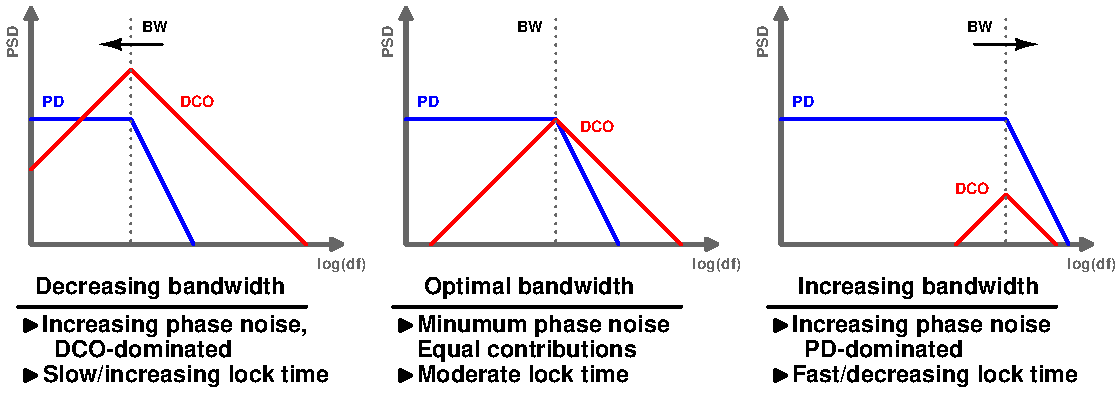
\includegraphics[width=1\textwidth, angle=0]{figs/theory/loop_bandwidth}
	% 		\caption{Bandwidth versus total integrated phase noise of PLL.}
	% 		\label{fig:bw_vs_pn2}
	% 	\end{figure}
	% 	\begin{figure}[htb!]
	%         \centering
	%         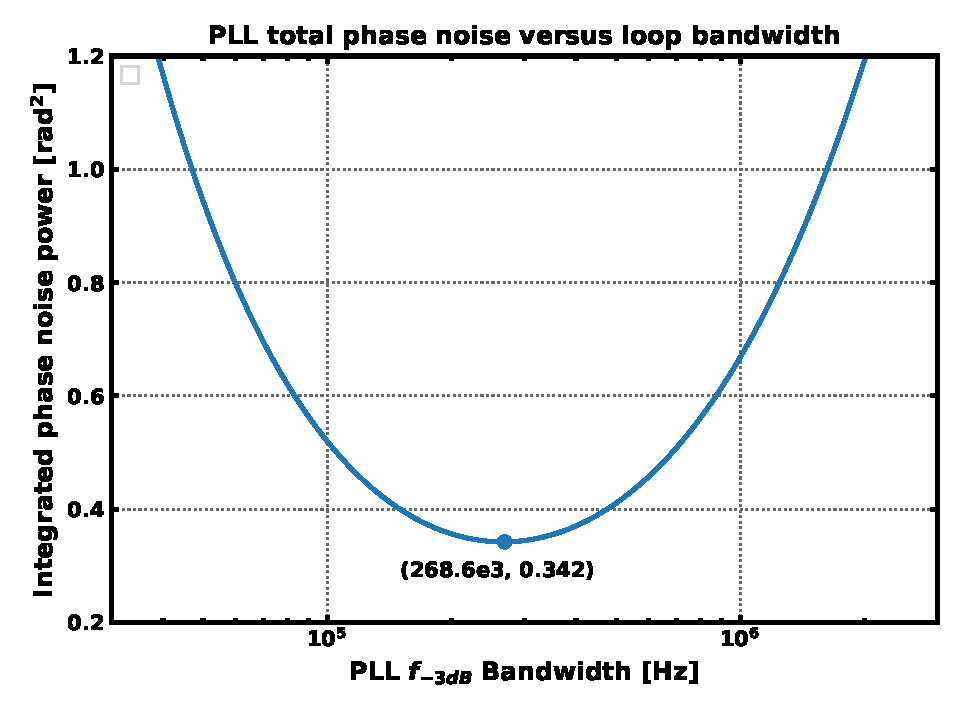
\includegraphics[width=0.6\textwidth, angle=0]{figs/bandwidth_vs_pn.pdf}
	% 	    \caption{Integrated phase noise power versus bandwidth for the same PLL.}
	% 	    \label{fig:pll_pn_opt_ex}
	% 	\end{figure}
\FloatBarrier{\color{white}.}
	% \input{theory2.tex}
	% \section{Methods}\label{methods}
	\FloatBarrier\newpage
	% The methods for implementation of a behavioral, discrete-time PLL simulator and for the PLL loop filter automation and optimization will be covered here.

% \hl{Talk about how simulator is implemented:}
% \hl{Discrete simulation models of phase noise, dco etc}
% \hl{Filter optimization}
% \hl{-phase noise and lock time estimate in frequency domain}
The primary objective in this work is to obtain a very low $100\mu$W power consumption for a 2.448 GHz PLL frequency synthesizer, while achieving a carrier-to-noise ratio for the synthesized signal of $>$20 dB. Consequently, the design philosophy adhered to in this work is pursue simplicity wherever possible, in order to reduce number of sources of power draw and noise. Furthermore, this design is targeted to allow duty cycled operation to further reduce power. Thus, an all-digital architecture has been selected to enable the possibility to save the PLL state, enter an ultra-low-power sleep state, and then resume from the stored state rapidly, without requiring relocking of the PLL. 

\subsection{Proposed Architecture - ADPLL}\label{pll_arch}
	The undertaken PLL architecture is in figure \ref{fig:pll_arch}. It comprises primarily of five components: (1) counter-based phase detector for initial start up, (2) bang-bang phase detector for steady state feedback, (3) proportional-integral controller loop filter, (4) DCO implemented as a VCO plus capacitive DACs, and (5) a control and calibration engine, consisting of digital logic. The rationale for this architecture will be described in the following subsections.
	\subsubsection{Block diagram}
			\begin{figure}[htb!]
		        \centering
		        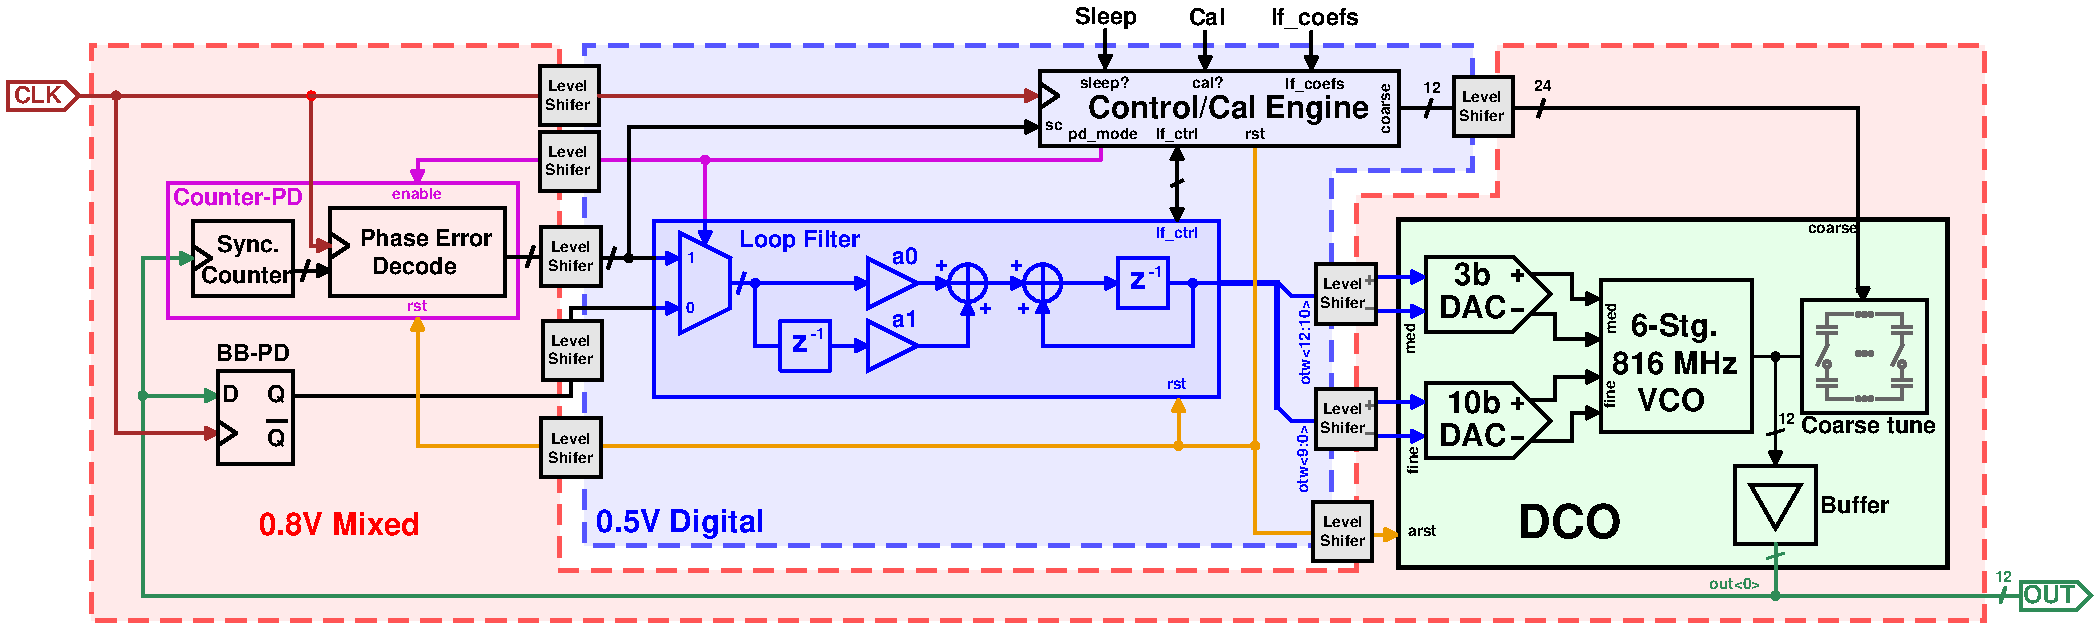
\includegraphics[width=1\textwidth, angle=0]{./figs/design/pll_master_arch_final}
			    \caption{ADPLL Architecture.}
			    \label{fig:pll_arch}
			\end{figure}

	\subsubsection{Power Saving Approach}
	Power savings have been attempted by minimization of complexity. First, the need of a divider is removed from the design by the usage of both the counter phase detector and BBPD. For initial cold start up of the PLL from an unknown state, the counter-based phase detector functions as a low-resolution replacement for a divider and linear phase detector. When near steady state, the counter-PD is disabled and replaced by BBPD feedback, which will maintain the PLL at steady state. The removal of a divider results in lower power consumption, and less noise added in-loop. The usage of only a BBPD in steady state further reduces power, as it is a minimum complexity phase detector. This is expected without significant performance degredation, as with proper optimization, BBPD PLLs can obtain comparable perform to linear charge-pump style PLLs \cite{xu_abidi_2017}. Additional power improvements are obtained in the usage of digital logic to implement the loop filter, using a simple PI-controller architecture. A divided power domain approach is used here, split between (1) 0.5V for loop filter, calibration and control logic, and (2) 0.8V for the analog portions, which constitute the DCO, in addition to the phase detectors. Multiple power domains allows for reduction of the digital logic power expenditure, while allowing for sufficient voltage for proper oscillator function. The final power saving move is implemented in a DCO based on the combination of several CDACs with a voltage controlled ring oscillator. This reduces to near zero the static curent draw associated with control of the VCO. The overall design is implemented with no static current paths, other than that associated with leakage, achieved by favoring static logic derived components throughout the PLL.

	\subsubsection{PLL Sleep Capability}
	A feature gained in the proposed all-digital architecture is the ability to abruptly save the state of the PLL digitally and place all unneeded components into an ultra low power sleep mode, and then later resume the PLL from the saved state. Figure \ref{fig:pll_sleep} demonstrate such operation, where $t_{l1}$ is the lock time from cold start, and $t_{l2}$ is the time to relock from a resume state. It is expected that slight drift in the oscillator characteristics will occur when resuming, so the relock time will likely be nonzero. However, the relock time is substantially lower than relocking from a cold state. This functionality enables the ability to rapidly duty cycle the PLL between active and sleep states. Power consumption of the PLL is reduced by a factor that is the duty cycle which it is operated; for example, 100$\mu$W nominal power consumption with 1\% duty cycle will result in 1$\mu$W average draw, which is attractive for wireless devices (particularly wake up radios).

			\begin{figure}[htb!]
			        \centering
			        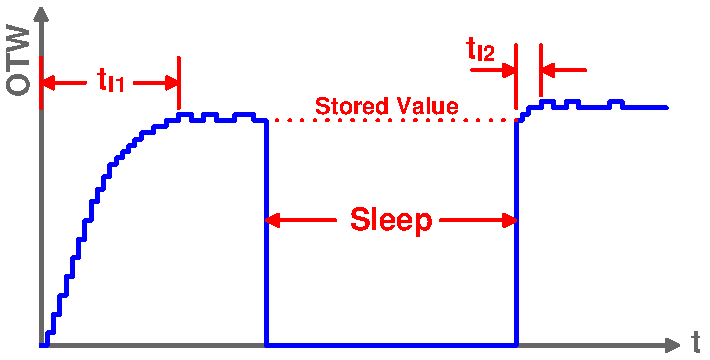
\includegraphics[width=0.6\textwidth, angle=0]{./figs/design/pll_sleep}
			    \caption{PLL sleep and resume operation.}
			    \label{fig:pll_sleep}
			\end{figure}


% \vspace{-2em}
% \begin{figure}[htb!]
% 	\center\fontfamily{\sfdefault}\selectfont
% XCircuit output "tdc_bbpll.tex" for LaTeX input from tdc_bbpll.ps
\def\putbox#1#2#3#4{\makebox[0.00000in][l]{\makebox[#1][l]{}\raisebox{\baselineskip}[0.00000in][0.00000in]{\raisebox{#2}[0.00000in][0.00000in]{\scalebox{#3}{#4}}}}}
\def\rightbox#1{\makebox[0.00000in][r]{#1}}
\def\centbox#1{\makebox[0.00000in]{#1}}
\def\topbox#1{\raisebox{-0.60\baselineskip}[0.00000in][0.00000in]{#1}}
\def\midbox#1{\raisebox{-0.20\baselineskip}[0.00000in][0.00000in]{#1}}
   \scalebox{1}{
   \normalsize
   \parbox{3.33750in}{
   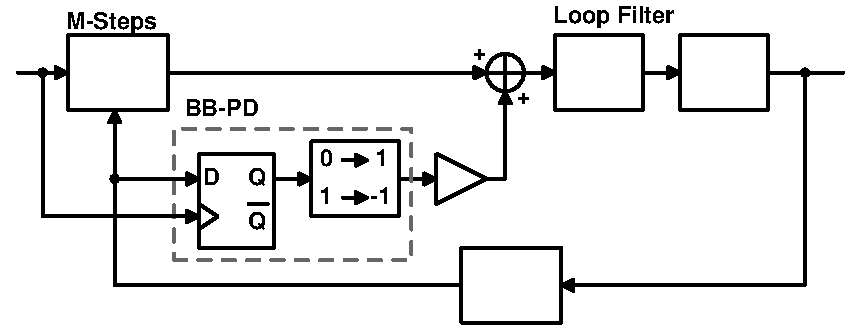
\includegraphics[scale=0.60000]{./figs/tdc_bbpll.pdf}\\
   % translate x=1412 y=528 scale 0.38
   \putbox{1.80600in}{0.70800in}{0.72}{$K_{bb}$}%
   \putbox{1.93200in}{0.14400in}{0.72}{$\div$ N}%
   \putbox{2.79600in}{0.99600in}{0.72}{DCO}%
   \putbox{2.24400in}{0.99600in}{0.72}{H$_{LF}$(z)}%
   \putbox{0.37200in}{0.99600in}{0.72}{TDC}%
   \putbox{0.03600in}{1.08600in}{0.72}{Clk}%
   \putbox{3.13200in}{1.08600in}{0.72}{Out}%
   } % close 'parbox'
   } % close 'scalebox'
   \vspace{-\baselineskip} % this is not necessary, but looks better
\fontfamily{\rmdefault}\selectfont

% 	\caption{PLL with parallel bang-bang phase detector and TDC.}
% 	\label{fig:tdc_bbpll}
% \end{figure}
	\subsubsection{Gear switching}
	The proposed digital architecture enables the ability to dynamically alter the loop filter response. This can be used to speed up lock from a cold state by using a lock time optimized filter initially, and then switch to a phase noise optimized filter after achieving initial lock. This approach is called gear switching \cite{staszewski_balsara_2007}, and is employed in this work by utilizing different loop filters for the start-up synchronous counter phase detector operation and the steady state BBPD operation.
	
	\subsubsection{Power budget}
	The below power budget was used in the design process to divide up the 100 $\mu$W allotment between the different PLL components. In order to minimize oscillator phase noise, as large of a portion was allotted to the oscillator, being 80\%. 
		\begin{table}[htb!]
			\centering
			\def\arraystretch{1.5}		
			\setlength\arrayrulewidth{0.75pt}
			\setlength{\tabcolsep}{1em} % for the horizontal padding
			\begin{tabular}{|c|c|c|c|c|}
				\hline 
				\rule[-1ex]{0pt}{2.5ex} \cellcolor{gray!40}\textbf{DCO} & \cellcolor{gray!40}\textbf{Phase detector} & \cellcolor{gray!40}\textbf{Digital (LF)}& \cellcolor{gray!40}\textbf{Other} & \cellcolor{gray!40}\textbf{SUM} \\ 
				\hline 
				\rule[-1ex]{0pt}{2.5ex} 80 $\mu$W& 10 $\mu$W &  10 $\mu$W  & 0 $ \mu$W & $\leq$ 100  $\mu$W\\ 
				\hline 
			\end{tabular} 
			\caption{Power budget for design process.}
			\label{tab:pow_budget}
		\end{table}   



	\subsubsection{Floorplan}
	The below floor plan (dimensions in microns) has been devised to meet the area requirement of $<$ 0.01 mm$^2$. The dimensions are 60$\mu$m x 85$\mu$m, with an area of 0.0051 mm$^2$. The yelow path demarcates the PLL loop signal flow. Attention was paid to separate analog (0.8V) and digital power domains (0.5V), whilst maintaining a compact area with convenient signal flow.
		\begin{figure}[htb!]
	        \centering
	        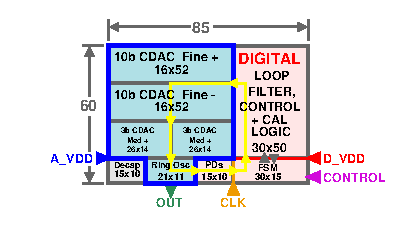
\includegraphics[width=0.75\textwidth, angle=0]{./figs/design/pll_floorplan3}
		    \caption{PLL floorplan.}
		\end{figure}

\subsubsection{Dividerless PLL}

\begin{figure}[htb!]
	\center\fontfamily{\sfdefault}\selectfont
% XCircuit output "bbpll_full_noise.tex" for LaTeX input from bbpll_full_noise.ps
\def\putbox#1#2#3#4{\makebox[0.00000in][l]{\makebox[#1][l]{}\raisebox{\baselineskip}[0.00000in][0.00000in]{\raisebox{#2}[0.00000in][0.00000in]{\scalebox{#3}{#4}}}}}
\def\rightbox#1{\makebox[0.00000in][r]{#1}}
\def\centbox#1{\makebox[0.00000in]{#1}}
\def\topbox#1{\raisebox{-0.60\baselineskip}[0.00000in][0.00000in]{#1}}
\def\midbox#1{\raisebox{-0.20\baselineskip}[0.00000in][0.00000in]{#1}}
   \scalebox{1}{
   \normalsize
   \parbox{5.50000in}{
   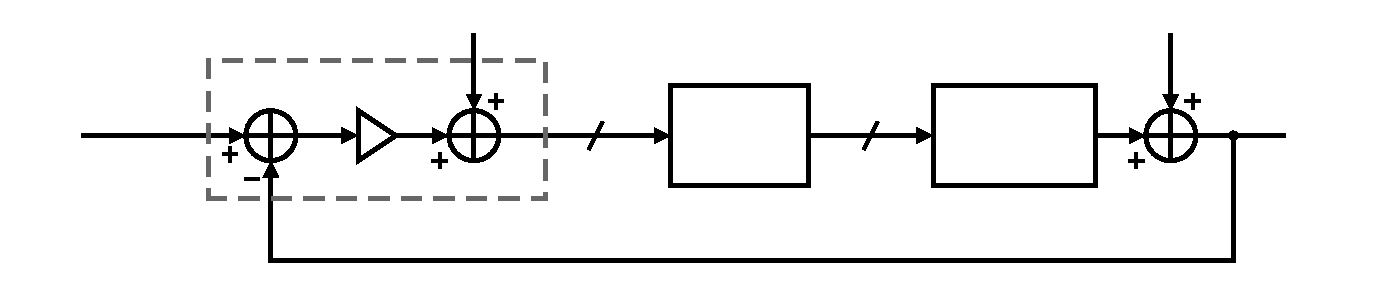
\includegraphics[scale=0.60000]{./figs/bbpll_full_noise.pdf}\\
   % translate x=416 y=448 scale 0.38
   \putbox{0.33600in}{0.70800in}{0.84}{$\Phi_{ref}$(t)}%
   \putbox{2.27400in}{0.73200in}{0.84}{e$_\Phi$(t)}%
   \putbox{1.42200in}{0.78600in}{0.84}{\rotatebox{-360}{$K_{BBPD}$}}%
   \putbox{1.20600in}{0.70800in}{0.84}{$\Phi_e$}%
   \putbox{0.83400in}{0.98400in}{0.84}{BBPD}%
   \putbox{2.77200in}{0.59400in}{0.84}{H$_{LF}$(s)}%
   \putbox{3.39600in}{0.72000in}{0.84}{u(t)}%
   \putbox{3.85800in}{0.60600in}{0.84}{$\frac{2\pi K_{DCO}}{s}$}%
   \putbox{4.82400in}{0.69600in}{0.84}{$\Phi_{out}$(t)}%
   \putbox{3.73200in}{0.87000in}{0.84}{DCO}%
   \putbox{1.93200in}{1.00800in}{0.84}{q$_{n_{BBPD}}$(t)}%
   \putbox{4.72200in}{1.00800in}{0.84}{$\Phi_{n_{DCO}}$(t)}%
   } % close 'parbox'
   } % close 'scalebox'
   \vspace{-\baselineskip} % this is not necessary, but looks better
\fontfamily{\rmdefault}\selectfont

	\caption{BBPD-PLL full noise model.}
	\label{fig:bbpll_full_noise}
\end{figure}

In the divider-based PLL theory (section \ref{sec:pll_output_noise}), the derived PLL detector phase noise component (equation \ref{eq:out_psd_bbpd_pll}) contains a term proportional to $N^2$, that is the detector noise will grow with the square of the PLL divider ratio. It is, however, possible to remove this $N^2$ dependency by usage of oscillator sub-sampling within the PLL \cite{Gao2015}. This is achieved by directly sampling the PLL output at a rate equivalent to the reference frequency. This is equivalent to removing the divider from the PLL loop and directly connecting the PLL output to the phase detector, which has been employed in this work (see figure \ref{fig:pll_arch}). The removal of the divider also removes any PLL noise contributions resulting from divider jitter. 

 In a dividerless PLL, it must be guaranteed that the PLL frequency at the start of sub-sampling operation be within $f_{ref}/2$ of the target frequency (the PLL will lock to the nearest multiple of the reference frequency). In this work, this is achieved through sequencing at startup through two phase detectors. A synchronous counter phase detector (which emulates both a divider and phase detector) initially locks the PLL within $f_{ref}/2$ of the target frequency, after which the PLL is operated in sub-sampling bang-bang phase detector.

  In accordance to the change to a dividerless operation, the PLL closed loop transfer function has been rederived in equation \ref{eq:cont_pll_tf2}. Furthermore, new expressions for PLL output phase noise with a BBPD is given in equation \ref{eq:out_psd_bbpd_pll2}, and PLL output oscillator noise with a ring oscillator is given in equation \ref{eq:out_psd_dco_pll2}, for the noise model in figure \ref{fig:bbpll_full_noise}. Noise due to the loop filter here is ignored, as it will be possible to adjust the loop filter datapath resolution to make digital quantizaiton noise effects negligible.
		\begin{align} \label{eq:cont_pll_tf2}
			\mathrm{T}(s) = \frac{\Phi_{out}(s)}{\Phi_{ref}(s)} = \frac{2\pi K_{BBPD}K_{DCO}\sum_{j=0}^Z b_js^j}{\sum_{k=0}^P a_ks^{k+1} + 2\pi K_{BBPD}K_{DCO}\sum_{j=0}^Z b_js^j} = \frac{\mathrm{L}(s)}{1 + \mathrm{L}(s)}
		\end{align}
		\begin{align}\label{eq:out_psd_bbpd_pll2}
			S_{\Phi n_{BBPD,out}}(f) &= S_{n_{BBPD}}(f)\left|\frac{\Phi_{out}(f)}{q_{n_{BBPD}}(f)}\right|^2 = \frac{\left(\frac{\pi}{2}-1\right)}{f_{ref}}\left|\sigma_{\Phi_e}\mathrm{T}(f)\right|^2
		\end{align}
		\begin{align}\label{eq:out_psd_dco_pll2}
			S_{\Phi n_{DCO,out}}(f) &= \mathcal{L}_{min}(f)\left|\frac{\Phi_{out}(f)}{q_{n_{DCO}}(f)}\right|^2 = \frac{7.33k_BT}{P}\left(\frac{f_0}{f}\right)^2|1-\textnormal{T}(f)|^2 
		\end{align}


% ################################################################################################
% ################################################################################################
	\subsection{Bang-Bang Phase Detector}
		A bang-bang phase detector, as introduced in section \ref{bbpd_theory}, can be implemented physically with a D flip-flop \cite{Razavi2020} and logic to map the logical state to a signed $\pm$1 value that may be passed into a digital loop filter. This is shown in figure \ref{fig:bbpd_dff}. 

		\begin{figure}[htb!]
			\center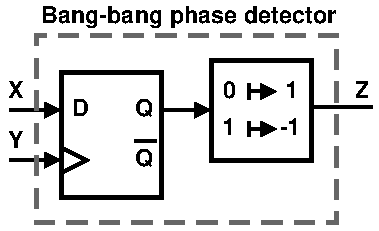
\includegraphics[width=0.4\textwidth, angle=0]{./figs/design/bbpd_}
			\caption{Bang-bang phase detector with D flip-flop.}
			\label{fig:bbpd_dff}
		\end{figure}
		The realization of a BBPD using a digital flip flop introduces additional noise to the system in the form of jitter. Jitter arises as an artifact of circuit and supply noise. For small time differentials between the BBPD inputs X and Y, the output can be stochatically corrupted due to the presence of noise. Furthermore, physical D flip flop implementations exhibit set-up and hold time requirements for data to be stable (to allow internal nodes to settle), so deterministic corruption of phase detection can be imparted if the inputs violate physical timing requirements. These sources of corruption cause BB-PD transfer characteristics in terms of output expectation, $\mathbb{E}[Z]$, with respect to input timing difference $\Delta t_{XY}$ to deviate from an ideal step response, demonstrated in figure \ref{fig:bbpd_jit_pdf}. Analytically, the corruption of the transfer characteristic can be viewed as being caused by an additive phase noise component before the signum operation in the BBPD, as shown in figure \ref{fig:bbpd_noise_nonlinear}. The expectation $\mathbb{E}[Z(\Delta t_{XY})]$ acts as a cumulative distribution function (CDF) for this phase noise component. Thus, differentiation of $\mathbb{E}[Z(\Delta t_{XY})]$ results in a probability distribution function (PDF) P(T=$\Delta t_{xy}$) of this phase noise signal. Statistical analysis of variance of the PDF provides an RMS value for timing jitter of this additive noise source, $\sqrt{\mathrm{Var}[T]} = \sigma_{t,j}$. The RMS timing jitter may be converted to RMS phase error of the noise source as $\sigma_{\Phi_j} = 2\pi f_{osc}\sigma_{t_j}$. This analysis approach is applied in this work to evaluate BBPD performance.
 
		\begin{figure}[htb!]
		    \centering
			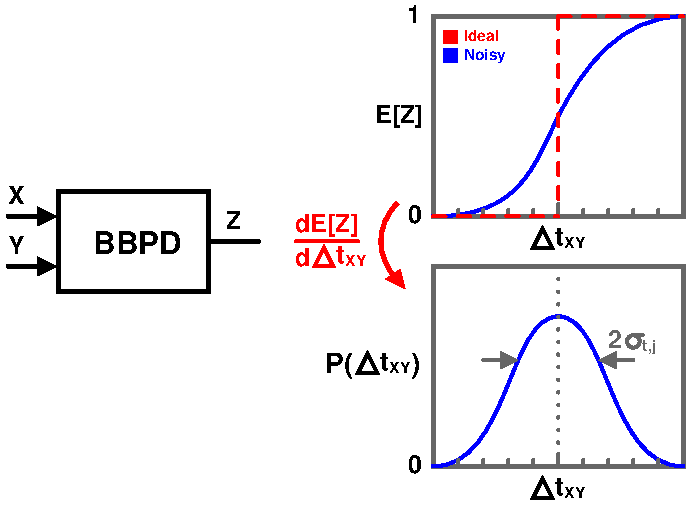
\includegraphics[width=0.6\textwidth, angle=0]{./figs/bbpd_jitter.pdf}
			\caption{BBPD output expectation and jitter PDF versus input time differential.}
			\label{fig:bbpd_jit_pdf}
		\end{figure}

	\begin{figure}[htb!]
	    \centering
	    \begin{subfigure}{0.5\textwidth}
	        \centering
	        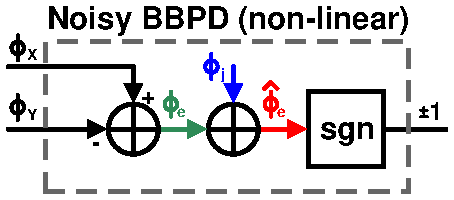
\includegraphics[width=0.8\textwidth, angle=0]{figs/design/bbpd_noise_nonlinear}
	        \caption{ }
	        \label{fig:bbpd_noise_nonlinear}
	    \end{subfigure}%
	    \begin{subfigure}{0.5\textwidth}
	        \centering
	        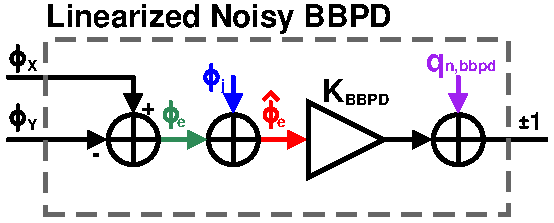
\includegraphics[width=0.9\textwidth, angle=0]{figs/design/bbpd_noise_linear}
	        \caption{ }
	        \label{fig:bbpd_noise_linear}
	    \end{subfigure}
	    % \caption{x.}
	    \caption{\textbf{(a)} Noisy BBPD nonlinear model \textbf{(b)} Noisy BBPD linearized model}
	     \label{fig:bbpd_noisy}
	\end{figure} 

	With a model for BBPD noise due to implementation non-idealities, a modified linearized model for the BBPD will be established here. This model will reconcile the ideal BBPD noise introduced in section \ref{sec:bbpd_noise} with the noise due to the new additive jitter component just described. First, a component representing the non-ideal jitter component, $\Phi_j$, is added into noise model from figure \ref{fig:bbpll_full_noise}. The result is the linearized model of figure \ref{fig:bbpd_noise_linear}. We then define a modified phase error, $\hat{\Phi}_e$, which includes the nominal $\Phi_e$ and the jitter corruption:
	\begin{equation}
	\hat{\Phi}_e = \Phi_e + \Phi_j.
	\end{equation}
	$\hat{\Phi}_e$ has a variance defined as $\sigma_{\hat{\Phi}_e}^2 = \sigma_{\Phi_e}^2 + \sigma_{\Phi_j}^2$, assuming $\Phi_e$ and $\Phi_j$ are uncorrelated. Defining BBPD gain in terms of $\sigma_{\hat{\Phi}_e}$:
	\begin{equation}
		K_{BBPD} = \sqrt{\frac{2}{\pi}}\cdot\frac{1}{\sigma_{\hat{\Phi}_e}} = \sqrt{\frac{2}{\pi}}\cdot\frac{1}{\sqrt{\sigma_{\Phi_e}^2 + \sigma_{\Phi_j}^2}}
	\end{equation}

	 It is then observed that the output Z is valued $\pm$1, thus its power is always $\sigma_Z^2$=1. Furthermore:
	\begin{equation}
	 	\sigma^2_{Z} = 1 = K_{BBPD}^2(\sigma^2_{\phi_e} +\sigma^2_{\phi_j})  + \sigma^2_{q_{n,BBPD}}
	\end{equation}
	 As determined in section \ref{sec:bbpd_noise}, it is inherent that $\sigma^2_{q_{n,BBPD}} = 1 - \frac{2}{\pi}$. If the total output noise
			\begin{equation}
				\sigma^2_{\phi_{n,BBPD}} =  \sigma^2_{q_{n,BBPD}} + K_{BBPD}^2\sigma^2_{\phi_j} =  1 - \frac{2}{\pi}\frac{\sigma^2_{\phi_e}}{\sigma^2_{\phi_j} + \sigma^2_{\phi_e}}
			\end{equation}
	If the BB-PD is connected directly to oscillator output, $\sigma^2_{\phi_e}$ = $\sigma^2_{\phi_n}$, i.e. the PLL output phase noise. The spectral density of the BB-PD phase noise is then:
		\begin{equation}
			S_{\phi_{n,BBPD}} = \frac{\sigma^2_{\phi_{n,BBPD}}}{f_{ref}} =  \frac{1 - \frac{2}{\pi}\frac{\sigma^2_{\phi_n}}{\sigma^2_{\phi_j} + \sigma^2_{\phi_n}}}{f_{ref}}
		\end{equation}

		\begin{align}\label{eq:out_psd_bbpd_pll3}
			S_{\Phi n_{BBPD,out}}(f) &= S_{n_{BBPD}}(f)\left|\frac{\Phi_{out}(f)}{q_{n_{BBPD}}(f)}\right|^2 = \frac{\frac{\pi}{2}(\sigma^2_{\phi_j} + \sigma^2_{\phi_n})-\sigma^2_{\phi_n}}{f_{ref}}\left|\mathrm{T}(f)\right|^2
		\end{align}

	% \begin{itemize}[itemsep=4pt,label=\protect---]
	% 	\item It is observed that PLL phase noise spectrum is approximately Lorentzian (except for peaking and flicker noise components). Given BB-PD noise PSD of $S_{\phi_{n,BBPD}}$, and an oscillator with noise PSD $S_{\phi_{n,osc}}(\Delta f)$, the optimal bandwidth for minimum noise power is:

	% 	\begin{equation}
	% 		BW_{opt} =  \sqrt{\frac{S_{\phi_{n,osc}}(\Delta f)}{S_{\phi_{n,BBPD}}}}\Delta f
	% 	\end{equation}
	% 	\item The total PLL output phase noise with optimal bandwidth is then:

	% 	\begin{equation}
	% 		\sigma^2_{\phi_{n,opt}} =   \pi\sqrt{\phi_{n,osc}(\Delta f)S_{\phi_{n,BBPD}}}\Delta f
	% 	\end{equation}
	% \end{itemize}
	% \vspace{-3em}
	% \begin{figure}[htb!]
	%     \centering
	%     \begin{subfigure}{0.33\textwidth}
	%         \centering
	%         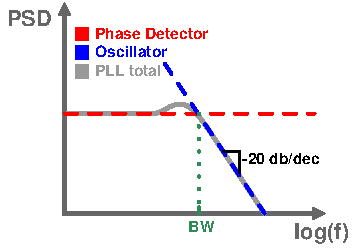
\includegraphics[width=1\textwidth, angle=0]{./figs/pll_spectrum_lorentzian.pdf}
	%     \end{subfigure}%
	%     \begin{subfigure}{0.33\textwidth}
	%         \centering
	%         \center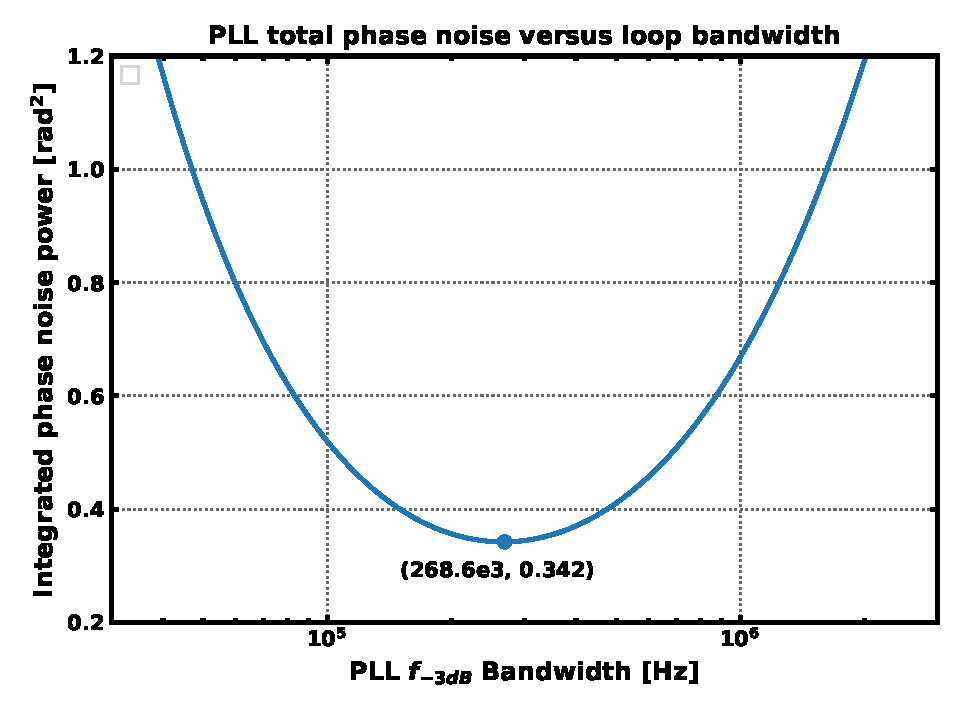
\includegraphics[width=1.0\textwidth, angle=0]{./figs/bandwidth_vs_pn.pdf}
	%     \end{subfigure}
	%     % \caption{Approximate model for ring oscillator inverter delay cell.}
	% \end{figure}




	% \begin{itemize}[itemsep=4pt,label=\protect---]
	% 	\item Using the findings for BB-PD noise PSD, assumption of Lorentzian spectrum, and constraint that BW = $\alpha f_{ref}$ (recommended $\alpha$$<$0.1 [2], rule of thumb since ancient PLL days). Given oscillator center frequency $f_c$, BB-PD jitter is constrained:

	% 	\begin{equation}
	% 		\sigma_{t_j} \leq \frac{\sigma_{\Phi_n}}{2\pi f_c}\sqrt{\frac{2}{\pi}\left(\frac{1}{\pi\alpha} - \frac{\pi}{2} + 1\right)} = \frac{\sigma_{\Phi_n}}{2\pi f_c}\beta(\alpha)
	% 	\end{equation}
	% 	\item $\beta(\alpha=0.1)$ = 1.28, $\beta(\alpha=0.05)$ = 1.92.
	% 	\item Using my PLL specifications ($f_c$ = 2.448 GHz, CNR = -$\sigma_{\Phi_n}$ = 17 dB, $\alpha=0.1$), {\color{red}\textbf{$\sigma_{t,j}\leq 11.8 $ ps}}
	% \end{itemize}



	% \begin{itemize}[itemsep=4pt,label=\protect---]
	% 	\item With an unconstrained relationship for BW and $f_{ref}$, and the optimal bandwidth finding, it is determined that the optimal value of $\sigma_{t,j}$ for minimum phase noise is:

	% 	\begin{equation}
	% 		\sigma_{t_j,opt} = \frac{\sigma_{\Phi_n}}{2\pi f_c}\sqrt{\frac{2}{\pi}\left[\frac{\sigma^4_{\Phi_n} f_{ref}}{\pi^2 S_{\phi_{n,osc}}(\Delta f) \Delta f^2} - \left(\frac{\pi}{2} - 1\right)\sigma^2_{\Phi_n}\right]}
	% 	\end{equation}

	% \end{itemize}

	% \begin{itemize}[itemsep=4pt,label=\protect---]
	% 	\item Setting the two jitter equations of the last side equal, it is found that optimal phase noise power is:

	% 	\begin{equation}
	% 		\sigma^2_{\Phi_n, opt} = \frac{\pi S_{\phi_{n,osc}}(\Delta f) \Delta f^2}{\alpha f_{ref}}
	% 	\end{equation}
	% 	\item The optimal reference frequency ($\sigma_{\Phi_n}=2\pi f_c \sigma_{t_n}$ = CNR):
	% 	\begin{equation}
	% 		f_{ref} = \frac{\pi S_{\phi_{n,osc}}(\Delta f) \Delta f^2}{\alpha \sigma^2_{\Phi_n}}
	% 	\end{equation}
	% 	\item The optimal oscillator phase noise at offset $\Delta f$:
	% 	\begin{equation}
	% 		S_{\phi_{n,osc}}(\Delta f) = \frac{\alpha f_{ref}\sigma^2_{\Phi_n}}{\pi \Delta f^2} 
	% 	\end{equation}
	% 	\item For CNR = 17 dB, $S_{\phi_{n,osc}}(\Delta f = 1 MHz)$ = -80 dBc/Hz, $\alpha$ = 0.1, {\color{red}the optimal $f_{ref}$ = 15.7 MHz.}
	% 	\item For CNR = 20 dB, $S_{\phi_{n,osc}}(\Delta f = 1 MHz)$ = -80 dBc/Hz, $\alpha$ = 0.1, {\color{red}the optimal $f_{ref}$ = 31.4 MHz.}
	% \end{itemize}


		\FloatBarrier






		\subsubsection{Circuit}
		The physcial implementation of the bang-bang phase detector has been selected to utilize a true single phase clock (TSPC) D-flip flop \cite{Yuan1989}. The positive-edge triggered variant of this circuit has been implemented as shown in figure \ref{fig:tspc_dff}. Selection of this topology was based on the desire for the usage of a single ended clock as a reference signal.

			\begin{figure}[htb!]
			        \centering
			        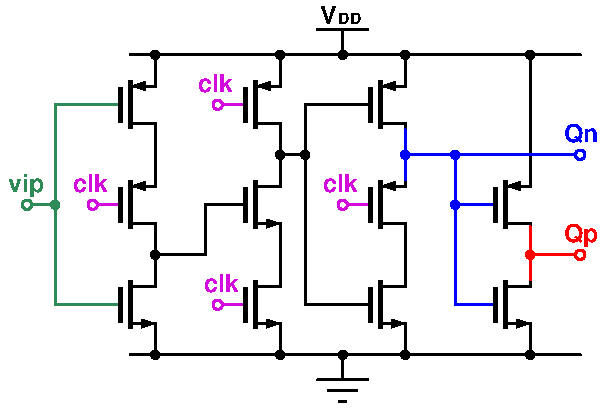
\includegraphics[width=0.6\textwidth, angle=0]{./figs/design/tspc_}
			    \caption{True single-phase clock (TSPC) D flip-flop, positive edge triggered.}
			    \label{fig:tspc_dff}
			\end{figure}

		This TSPC design was validated in simulation with RVT devices with all devices set with (W/L) = \{100n/20n, 200n/20n\}, and with supply voltages of 0.5 and 0.8 volts. Results for the RMS jitter and power consumption are in table \ref{tab:dff}. For implementation (W/L) = 200n/20n was selected for all devices, as the requirement of 10 $\mu$W is met with layout parasitics, whilst having low jitter.


		% \end{itemize}
		% % \vspace{-3em}
		% \begin{figure}[htb!]
		%     \centering
		%     \begin{subfigure}{0.5\textwidth}
		%         \centering
		%         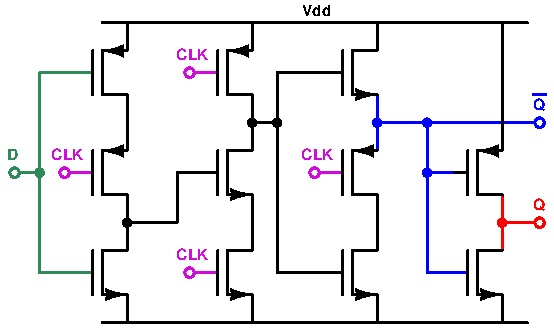
\includegraphics[width=0.8\textwidth, angle=0]{./figs/tspc_dff.pdf}
		%         \caption{TSPC DFF}
		%     \end{subfigure}%
		%     \begin{subfigure}{0.5\textwidth}
		%         \centering
		%         \center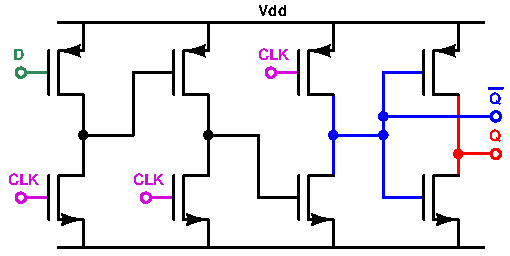
\includegraphics[width=0.8\textwidth, angle=0]{./figs/etspc_dff.pdf}
		%         \caption{e-TSPC DFF}
		%     \end{subfigure}
		%     % \caption{Approximate model for ring oscillator inverter delay cell.}
		% \end{figure}


	% \begin{itemize}[itemsep=4pt,label=\protect---]
	% 	\item Utilized TSPC DFF, with inverter buffers (FETs sized 200n/20n) for clock and data buffers.
	% 	\item Sweep delay between inputs, calculating the expect value of the output for 100 bits. Transient noise simulated (up to 100 GHz), and the inital state of the FF is set to be high 50x and low 50x to include hysteresis effects. 
	% 	\item V$_{DD} \in$ \{0.5, 0.8\} V and (W/L) $\in$ \{100n/20n, 200n/20n\} tested. 100 aF added to every node.
	% 	\item \textbf{Resulting CDFs of the input time delta versus output expectation are below.}
	% \end{itemize}
	% \vspace{-2em}
	% \begin{figure}[htb!]
	%     \centering
	% 	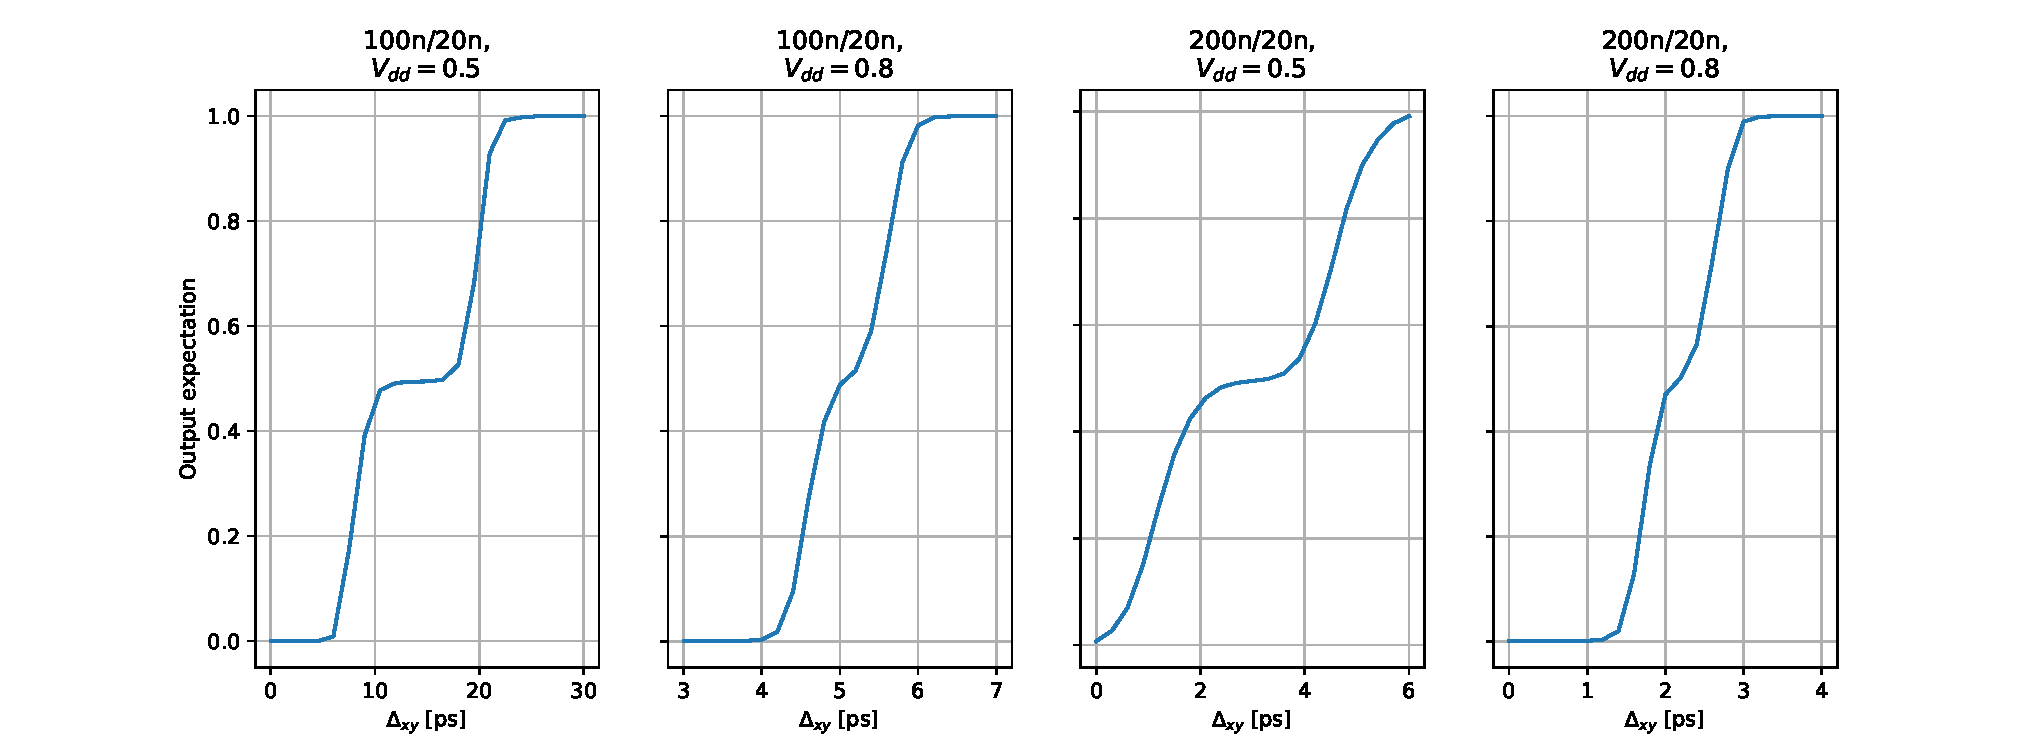
\includegraphics[width=1\textwidth, angle=0]{./figs/cdfs.pdf}
	% \end{figure}

	% \begin{itemize}[itemsep=4pt,label=\protect---]
	% 	\item Jitter PDFs are bimodal from hysteresis of DFF. 
	% 	\item Increasing (W/L) or $V_{DD}$ both impact jitter favorably.
	% 	\item \textbf{The jitter PDF (computed from the CDFs) of the input time delta versus output expectation are below. (Delays are removed)}
	% \end{itemize}
	% \vspace{-2em}
	% \begin{figure}[htb!]
	%     \centering
	% 	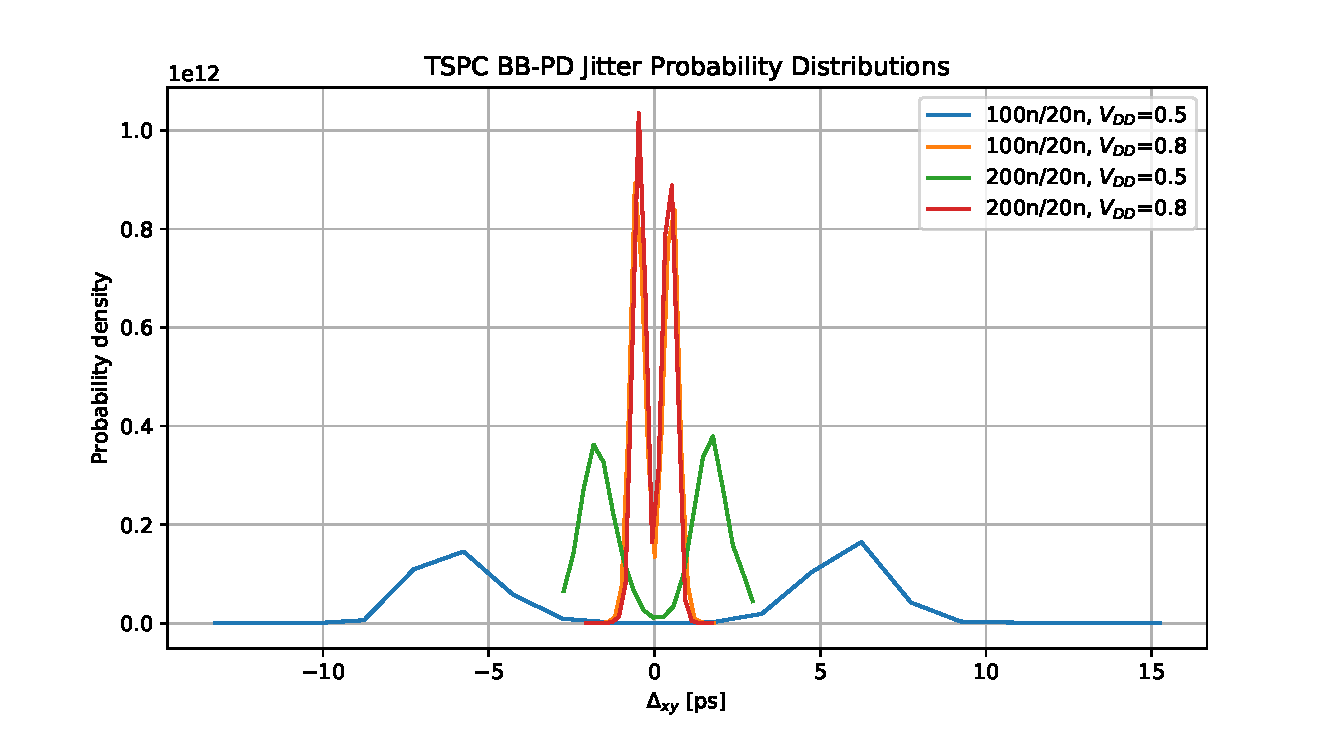
\includegraphics[width=0.7\textwidth, angle=0]{./figs/jitter_pdfs.pdf}
	% 	\caption{Jitter PDF from simulated TSPC DFFs.}
	% 	\label{fig:tspc_dff_sim}
	% \end{figure}


		\begin{table}[h!]
			\centering
			\def\arraystretch{1.5}		
			\setlength\arrayrulewidth{0.75pt}
			\setlength{\tabcolsep}{1em} % for the horizontal padding
			\begin{tabular}{|c|c|c|c|}
				\hline 
				\rule[-1ex]{0pt}{2.5ex} \cellcolor{gray!40}\textbf{(W/L)} & \cellcolor{gray!40}\textbf{Supply [V]} & \cellcolor{gray!40}\textbf{RMS jitter [ps]}& \cellcolor{gray!40}\textbf{Power [$\mu$W]}\\ 
				\hline 
				\rule[-1ex]{0pt}{2.5ex} 100n/20n  & 0.5 & 6.01 & 1.64\\ 
				\hline 
				\rule[-1ex]{0pt}{2.5ex} 100n/20n  & 0.8 & 0.832  & 3.942\\ 
				\hline 
				\rule[-1ex]{0pt}{2.5ex} 200n/20n  & 0.5 & 1.776 & 2.215 \\ 
				\hline 
				\rule[-1ex]{0pt}{2.5ex} 200n/20n  & 0.8 & 0.496  & 4.591 \\ 
				\hline 
			\end{tabular} 
			\caption{Schematic simulation of TSPC DFF.}
			\label{tab:dff}
		\end{table}   
		\FloatBarrier{\color{white}.}







		% \FloatBarrier
		% \subsubsection{Layout}
		% 	\hl{Area?}
		% 	\begin{figure}[htb!]
		% 	        \centering
		% 	        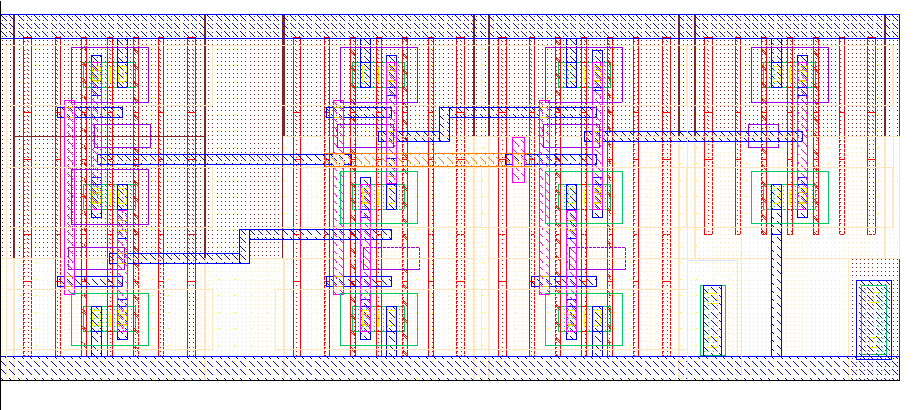
\includegraphics[width=\textwidth, angle=0]{./figs/layout/layout_bbpd}
		% 	    \caption{Single ended bang-bang phase detector.}
		% 	\end{figure}

% ################################################################################################
% ################################################################################################


\FloatBarrier\pagebreak
\subsection{Voltage Controlled Ring oscillator}
	Oscillator circuits implemented in CMOS technology either fall under the catagory of resonant LC circuits, or RC based ring and relaxation oscillators. LC circuits provide favorable phase noise performance, as seen in figure \ref{fig:lc_ro_fom}, which demonstrates phase noise improvements on the order of 20 dB for LC designs over RC designs that have been published. This is due to the inherent nature of an LC circuit, as the higher the quality factor it has, the narrower the resonance line width and consequent phase noise is. In the ultra-low power domain of this work, however, ring oscillators pose several advantages over LC designs. These include substantially smaller integration area due to no need for integrated inductors, simpler design, convenient rail-to-rail signal levels, and lower achievable minimum power at a given frequency. Also significant, is the ability to instantly start up a ring oscillator, which can be achieved with known phase if using appropriate reset circuitry. Coupled with the BBPD, which is a phase only detector (which is not able to detect frequency), the ability to start the oscillator with a known zero-phase, in tandem with being able to set the digital loop filter to a zeroed state, enables faster and more consistant locking compared to randomized initial phase. With the intent of this design to allow for fast duty cycled operation, the need for fast start up is imperative, thus for this reason the ring oscillator topology has been selected for this work. 

	It has been decided in this work to exploit the ability of the FD-SOI backgate terminal to alter threshold voltage in order to implement a backgate voltage controlled ring oscillator as the main PLL VCO. As will be shown in the following sections, backgate tuning results in transconductor modulation within the ring oscillator, which therefore modulates the RC time constant of the delay stages, and consequently the frequency of oscillation. A novel delay cell topology which exploits FD-SOI backgates to implement both differential operation and frequency is subsequently introduced. The described design enables usage of capacitive DACs to set oscillator control voltages, leading to minimal extra power consumption needed to convert the voltage controlled ring oscillator into a DCO. 




			\FloatBarrier
	\subsubsection{22FDX considerations}
		To analyze the body effect through FD-SOI backgates in 22FDX, SPICE simulations to extract the body effect coefficient $\gamma$ and theshold voltage $V_{TH}$ for different channel lengths and bias conditions have been performed. Parameters for threshold voltage, and transconductances $g_m$ and $g_{mb}$ have been extracted using DC operating point simulations. Noting the relation from \ref{eq:gm_gmb_relation}, where $g_{mb} = \gamma g_{m}$, $\gamma$ can be deduced from operating point $g_m$ and $g_{mb}$ values. Figures \ref{fig:vth_vs_vbs} and \ref{fig:vth_slope_vs_vbs} show the extracted threshold voltage versus backgate bias and the slope of that relationship. Figures \ref{fig:vth_vs_len} and \ref{fig:gamma_vs_len} show the extracted theshold voltage and body effect coefficient versus channel length. Table \ref{tab:nfet_vth_gamma} provides extracted N-channel device parameters, and table \ref{tab:pfet_vth_gamma} provides extracted P-channel devices parameters.

		It is observed that the threshold voltage slopes of figure \ref{fig:vth_groupa} are not perfectly linear, but for the simplified analytical purposes of this work, they can be approximated as linear. The P-channel devices in 22FDX show a high degree of linearity, whereas the N-channel devices show variation in slope as in figure \ref{fig:vth_slope_vs_vbs}. It is also observed that the threshold voltage and body effect coefficient vary as channel lengths approach zero, but flatten out for longer device length. A final note is there is substantial variation of $\gamma$ and $V_{TH}$ between device types, so prudent care must be taken in the oscillator for selection of devices and their sizing.

		\begin{equation}
		V_{th} = V_{th0} - \gamma V_{BS}
		\end{equation}

		\begin{figure}[htb!]
		    \centering
		    \begin{subfigure}{0.5\textwidth}
		        \centering
		        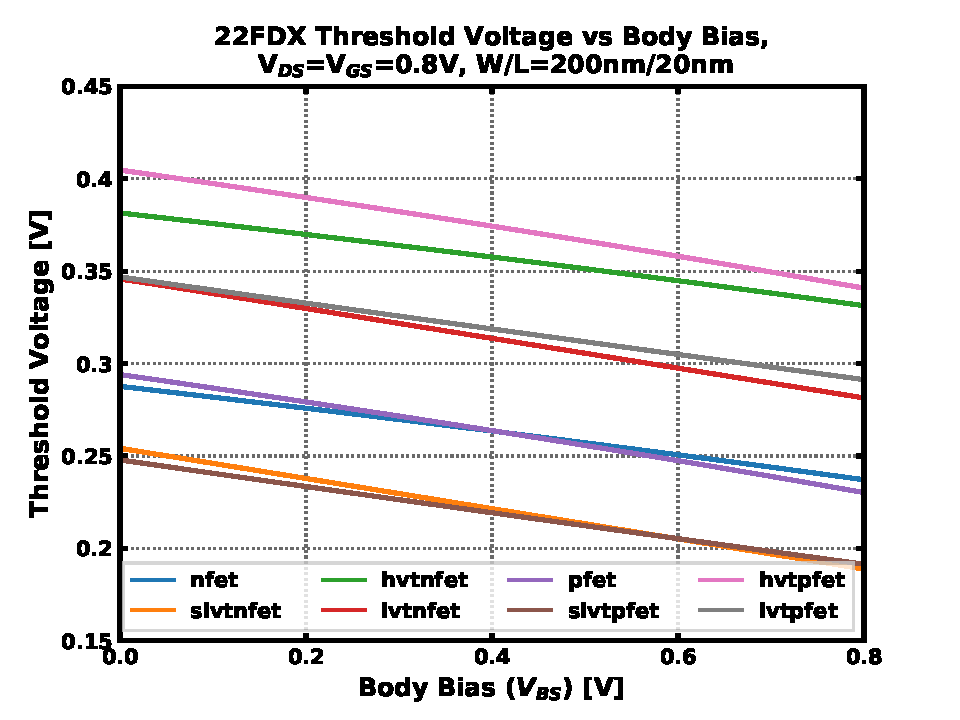
\includegraphics[width=1\textwidth, angle=0]{./figs/design/vth_vbs}
		        \caption{ }
		        \label{fig:vth_vs_vbs}
		    \end{subfigure}%
		    \begin{subfigure}{0.5\textwidth}
		        \centering
		        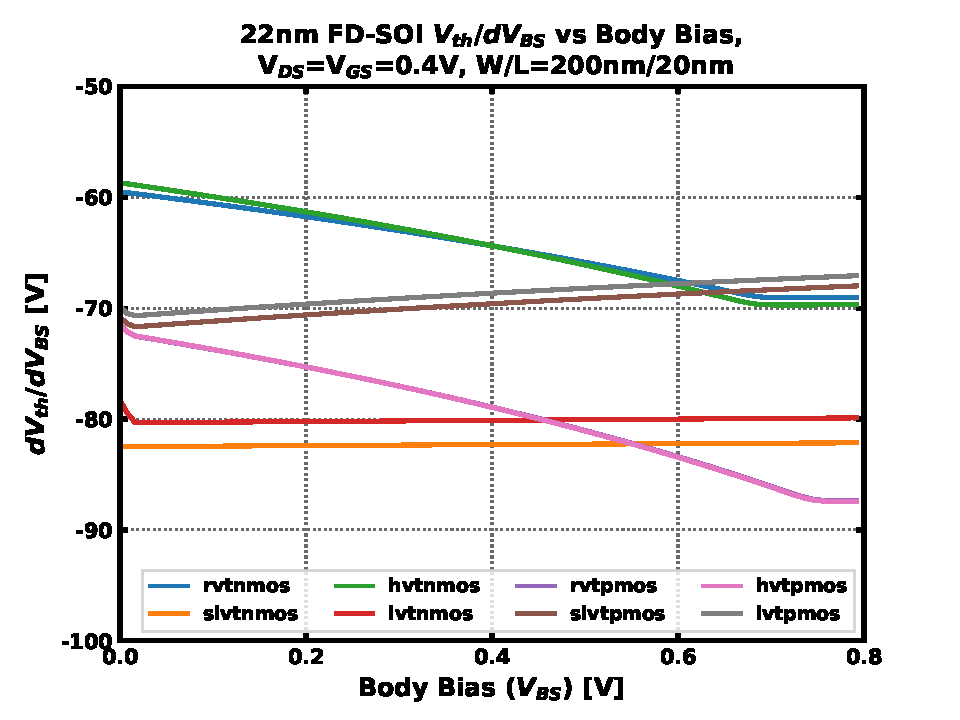
\includegraphics[width=1\textwidth, angle=0]{./figs/design/vth_slope_vbs}
		        \caption{ }
		        \label{fig:vth_slope_vs_vbs}
		    \end{subfigure}
		    % \caption{x.}
		    \caption{\textbf{(a)} 22 FDX threshold voltage versus body bias, \textbf{(b)} Rate of change of threshold voltage versus body bias.}
		    \label{fig:vth_groupa}
		\end{figure} 


		\begin{figure}[htb!]
		    \centering
		    \begin{subfigure}{0.5\textwidth}
		        \centering
		        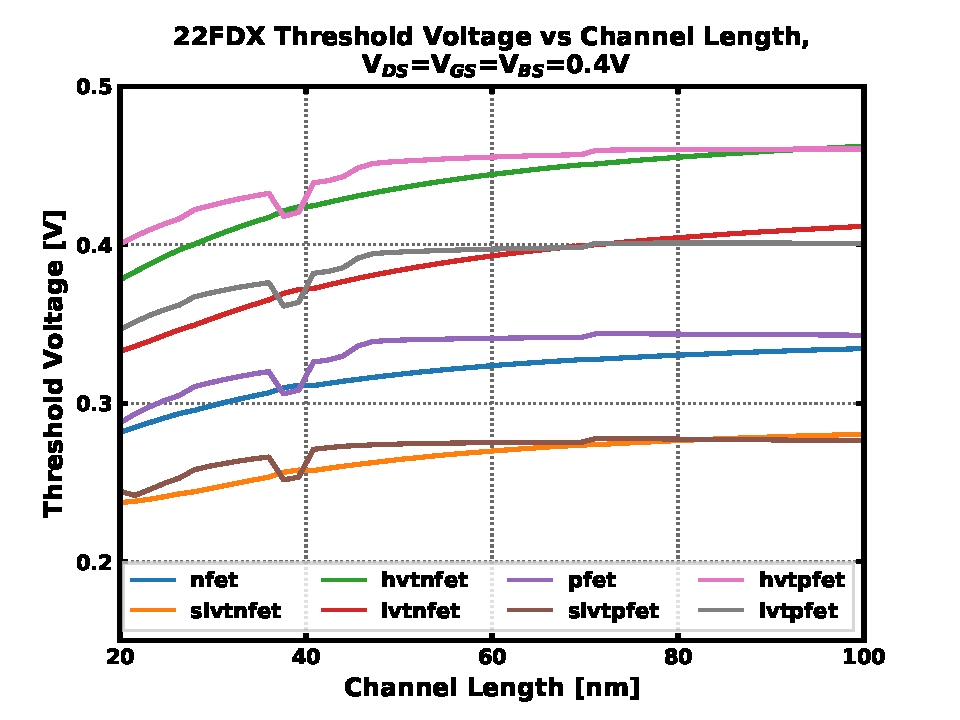
\includegraphics[width=1\textwidth, angle=0]{./figs/design/vth}
		        \caption{ }
		        \label{fig:vth_vs_len}
		    \end{subfigure}%
		    \begin{subfigure}{0.5\textwidth}
		        \centering
		        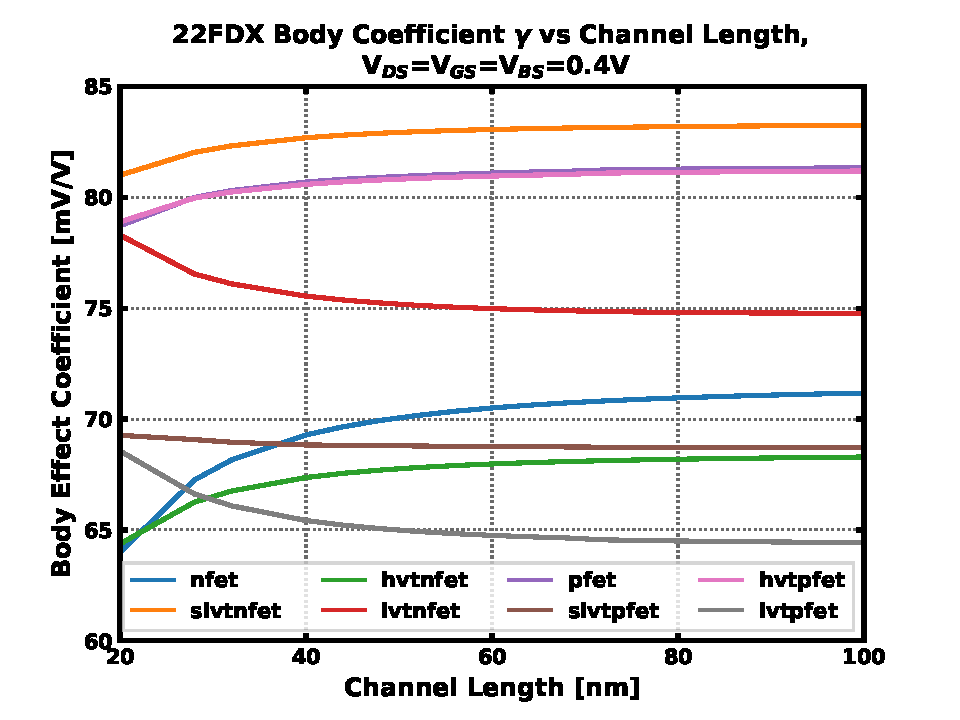
\includegraphics[width=1\textwidth, angle=0]{./figs/design/gamma}
		        \caption{ }
		        \label{fig:gamma_vs_len}
		    \end{subfigure}
		    % \caption{x.}
		    \label{fig:vth_groupb}
		    \caption{\textbf{(a)} 22 FDX Extracted threshold voltage versus channel length, \textbf{(b)} Extracted body effect coefficient.}
		\end{figure} 


			\begin{table}[htb!]
				\centering
				\def\arraystretch{1.5}		
				\setlength\arrayrulewidth{1pt}
				\setlength{\tabcolsep}{1em} % for the horizontal padding
				\fontfamily{\sfdefault}\selectfont 
				\begin{tabular}{|l|l|l|l|l|}	
					\hline 
					\rule[-1ex]{0pt}{2.5ex} \cellcolor{gray!40}\textbf{Device} & \cellcolor{gray!40}\textbf{L [nm]} & \cellcolor{gray!40}\textbf{W [nm]} & \cellcolor{gray!40}\textbf{$V_{th}$ [mV]} & \cellcolor{gray!40}\textbf{$\gamma$ [mV/V]}\\ 
					\hline 
					\rule[-1ex]{0pt}{2.5ex} \textbf{nfet} & 20 & 100 & 306.3 & 59.14 \\ 
					\hline 
					\rule[-1ex]{0pt}{2.5ex} \textbf{nfet} & 100 & 500 & 376.4 & 65.4 \\ 
					\hline 
					\rule[-1ex]{0pt}{2.5ex} \textbf{slvtnfet} & 20n & 100 & 270.3 & 81.38 \\ 
					\hline 
					\rule[-1ex]{0pt}{2.5ex} \textbf{slvtnfet} & 100 & 500 & 326.7 & 83.23 \\ 
					\hline 
					\rule[-1ex]{0pt}{2.5ex} \textbf{hvtnfet} & 20n & 100 & 402.4 & 58.85 \\ 
					\hline 
					\rule[-1ex]{0pt}{2.5ex} \textbf{hvtnfet} & 100 & 500 & 513.5 & 61.96 \\ 
					\hline 
					\rule[-1ex]{0pt}{2.5ex} \textbf{lvtnfet} & 20 & 100 & 364.9 & 77.72 \\ 
					\hline 
					\rule[-1ex]{0pt}{2.5ex} \textbf{lvtnfet} & 100 & 500 & 466.3 & 74.85 \\ 
					\hline 
				\end{tabular} 
				\caption{22FDX core NFET threshold voltage and body effect coefficient extraction.}
				\label{tab:nfet_vth_gamma}
			\end{table} 

			\begin{table}[htb!]
				\centering
				\def\arraystretch{1.5}		
				\setlength\arrayrulewidth{1pt}
				\setlength{\tabcolsep}{1em} % for the horizontal padding
				\fontfamily{\sfdefault}\selectfont 
				\begin{tabular}{|l|l|l|l|l|}	
					\hline 
					\rule[-1ex]{0pt}{2.5ex} \cellcolor{gray!40}\textbf{Device} & \cellcolor{gray!40}\textbf{L [nm]} & \cellcolor{gray!40}\textbf{W [nm]} & \cellcolor{gray!40}\textbf{$V_{th}$ [mV]} & \cellcolor{gray!40}\textbf{$\gamma$ [mV/V]}\\ 
					\hline 
					\rule[-1ex]{0pt}{2.5ex} \textbf{pfet} & 20 & 100 & 317.7 & 71.51 \\ 
					\hline 
					\rule[-1ex]{0pt}{2.5ex} \textbf{pfet} & 100 & 500 & 366.8 & 74.32 \\ 
					\hline 
					\rule[-1ex]{0pt}{2.5ex} \textbf{slvtpfet} & 20n & 100 & 272.6 & 71.09 \\ 
					\hline 
					\rule[-1ex]{0pt}{2.5ex} \textbf{slvtpfet} & 100 & 500 & 294.4 & 70.79 \\ 
					\hline 
					\rule[-1ex]{0pt}{2.5ex} \textbf{hvtpfet} & 20n & 100 & 430.7 & 71.28 \\ 
					\hline 
					\rule[-1ex]{0pt}{2.5ex} \textbf{hvtpfet} & 100 & 500 & 488.4 & 74.23 \\ 
					\hline 
					\rule[-1ex]{0pt}{2.5ex} \textbf{lvtpfet} & 20 & 100 & 374.2 & 69.93 \\ 
					\hline 
					\rule[-1ex]{0pt}{2.5ex} \textbf{lvtpfet} & 100 & 500 & 422.8 & 66.43 \\ 
					\hline 
				\end{tabular} 
				\caption{22FDX core PFET threshold voltage and body effect coefficient extraction.}
				\label{tab:pfet_vth_gamma}
			\end{table} 	
\FloatBarrier

\subsubsection{Channel length consideration}
	Scaling of device channel length has a great impact on phase noise for ring oscillators, according to \cite{Liu2020} takes form of equation \ref{eq:liu_pn_scaling}. $V_{DD}$ is the supply voltage, $V_t$ is the threshold voltage, $P_{DC}$ is the oscillator power consumption, $\gamma p$ and $\gamma n$ are the respective PMOS and NMOS noise factors, $f_0$ is the oscillator frequency, and $f$ is the offset from the carrier for the phase noise. It is expected that excess noise factor of the transistor will increase with decreasing channel length \cite{Antonopoulos2013}, thus unavoidably phase noise will also increase with decreasing length following equation \ref{eq:liu_pn_scaling}. To analyze the effect of channel length on ring oscillator performance in 22FDX technology, a 5-stage single ended ring oscillator was simulated for channel lengths between 20-500nm, with a fixed (W/L)=5 and no external loading. The resulting phase noise FOM$_{pn}$ data is shown in figure \ref{fig:rosc_fom}, oscillator frequency in figure \ref{fig:rosc_freq}, oscillator power in figure \ref{fig:rosc_power}, and phase noise at offset 1 MHz from the carrier in figure \ref{fig:rosc_pn_1m}. The phase noise FOM is that defined in equation \ref{eq:fom_pn}. It is seen that FOM degrades as expected near minimum channel length, and improves asymptotically as the channel length grows. The asymptote closely correlates to that predicted theoretically for RC based oscillators, in equation \ref{eq:ro_fom_limit}. At 300K, as simulated, this is -165.2 dB. Better (i.e. lower valued) FOM corresponds to better phase noise per unit of oscillator power expenditure. Thus, based on the data of figure \ref{fig:rosc_fom}, the best design strategy to minimize phase noise for a fixed power budget is to use the longest possible channel length. Channel length limits frequency of operation, as seen in figure \ref{fig:rosc_freq}, so there is a trade off between frequency of operation and achievable FOM. 

	\begin{equation} \label{eq:liu_pn_scaling}
		\mathcal {L}(f) =\frac {2kT}{P_{\textrm {DC}}}\left ({\frac {V_{\textrm {DD}}}{V_{\textrm {DD}}-V_{t}} (\gamma _{N}+\gamma _{P}+1)}\right)\left ({\frac {f_{0}}{f}}\right)^{2}
	\end{equation}

		\begin{figure}[htb!]
		    \centering
		    \begin{subfigure}{0.5\textwidth}
		        \centering
		        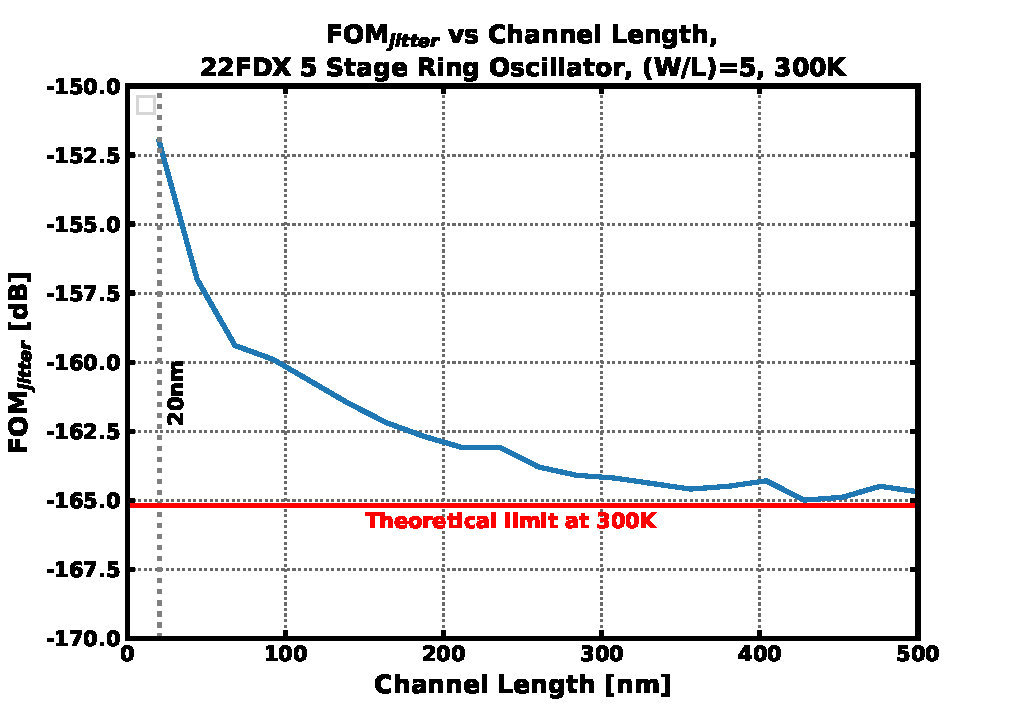
\includegraphics[width=1\textwidth, angle=0]{./figs/design/22fdx_rosc_fom}
		        \caption{ }
		        \label{fig:rosc_fom}
		    \end{subfigure}%
		    \begin{subfigure}{0.5\textwidth}
		        \centering
		        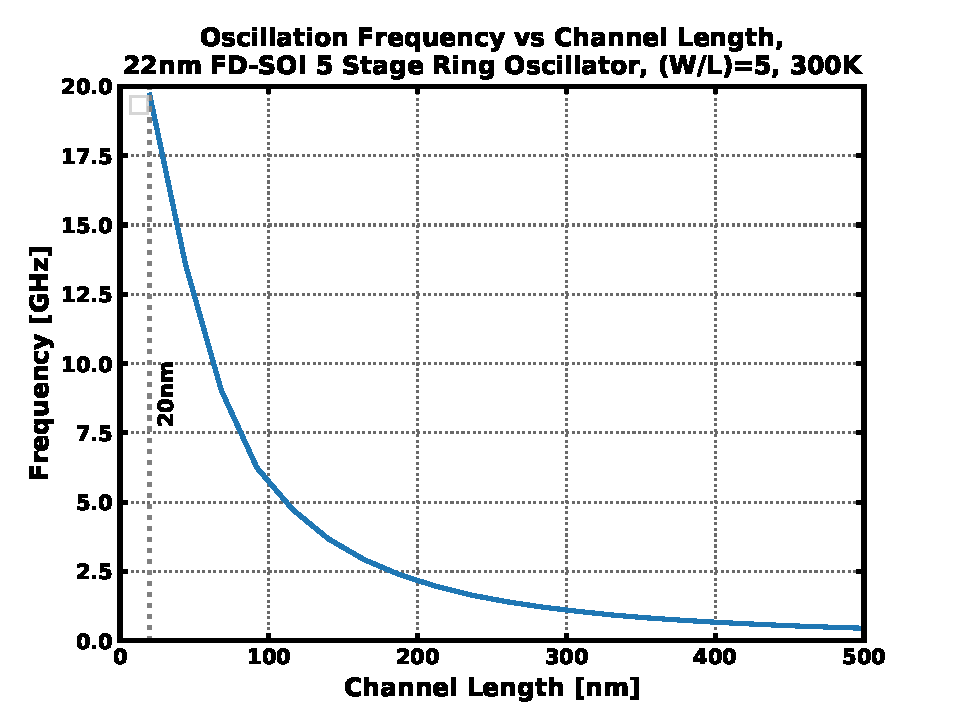
\includegraphics[width=1\textwidth, angle=0]{./figs/design/22fdx_rosc_freq}
		        \caption{ }
		        \label{fig:rosc_freq}
		    \end{subfigure}
		    % \caption{x.}
		    \label{fig:rosc_groupa}
		    \caption{22FDX ring oscillator channel length sweep versus \textbf{(a)} FOM, \textbf{(b)} Oscillation frequency.}
		\end{figure} 	

		\begin{figure}[htb!]
		    \centering
		    \begin{subfigure}{0.5\textwidth}
		        \centering
		        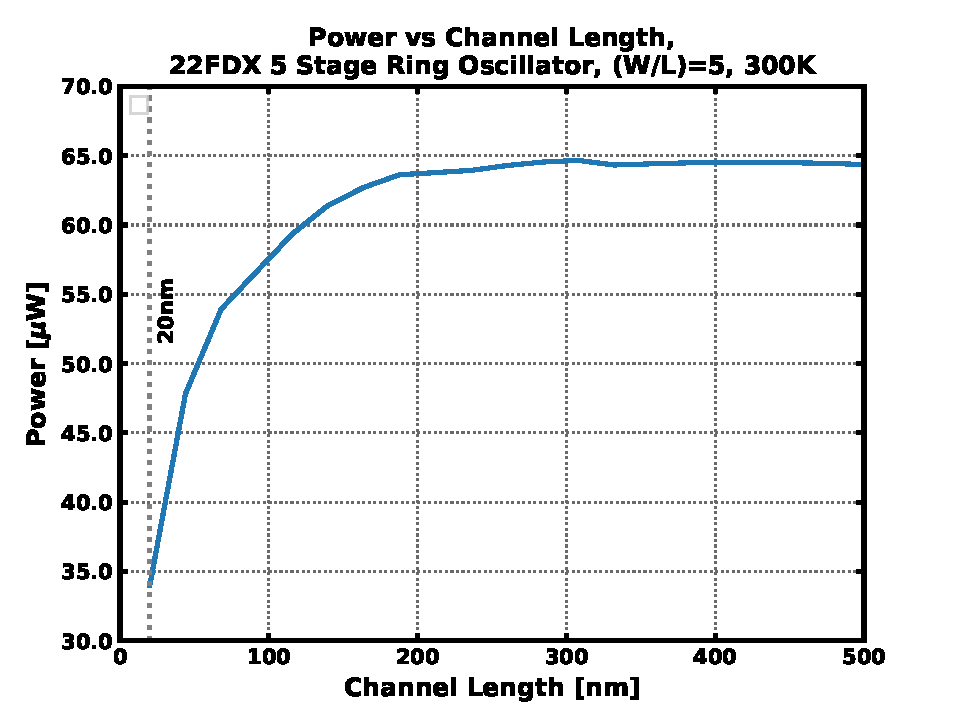
\includegraphics[width=1\textwidth, angle=0]{./figs/design/22fdx_rosc_power}
		        \caption{ }
		        \label{fig:rosc_power}
		    \end{subfigure}%
		    \begin{subfigure}{0.5\textwidth}
		        \centering
		        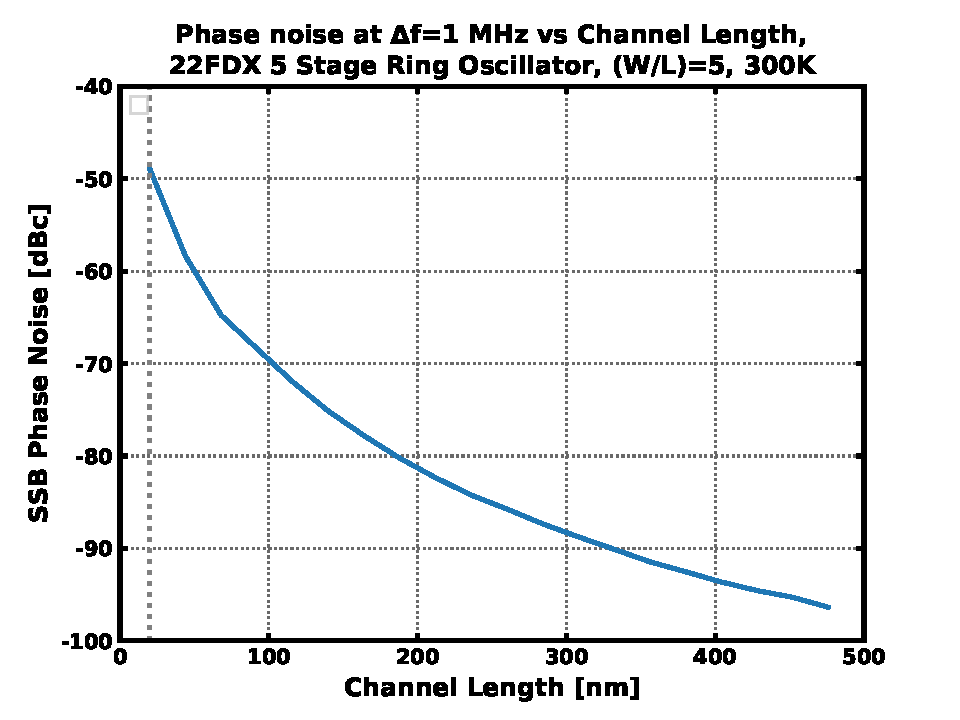
\includegraphics[width=1\textwidth, angle=0]{./figs/design/22fdx_rosc_pn_1mhz}
		        \caption{ }
		        \label{fig:rosc_pn_1m}
		    \end{subfigure}
		    % \caption{x.}
		    \label{fig:rosc_groupb}
		    \caption{22FDX ring oscillator channel length sweep versus \textbf{(a)} Power, \textbf{(b)} Phase noise at 1 MHz carrier offset (SSB).}
		\end{figure} 

	\FloatBarrier


	\subsubsection{Ring oscillator frequency derivation}
		To analyze the effect of backgate tuning on a FD-SOI ring oscillator, a general mathematical model for CMOS ring oscillators will be developed first here. To begin, an approximate model for a CMOS inverter will first be considered. A common model for delay in digital circuits is an RC circuit, where the MOSFET channels are approximated with an averaged conductance value $\langle g_{ch} \rangle$, and the output node is approximated to have a capacitance of C. With such a model, a ring oscillator would be assumed to have waveforms as decaying exponential, with time constant $\tau = \langle g_{ch} \rangle^{-1}C$. In context of the 3-stage ring oscillator of figure \ref{fig:rosc_rc}, figure \ref{fig:inv_model} demonstrates the described inverter model and the resulting input and output waveforms.

		\begin{figure}[htb!]
			\center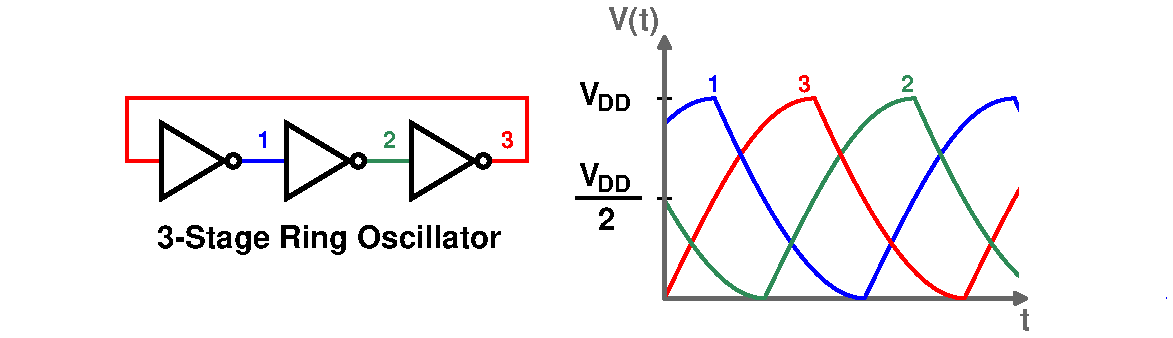
\includegraphics[width=0.8\linewidth, angle=0]{figs/theory/osc_waves}
			\caption{Model for ring oscillator.}
			\label{fig:rosc_rc}
		\end{figure}

		\begin{figure}[htb!]
	        \centering
	        \begin{subfigure}{.5\textwidth}
	            \centering
	            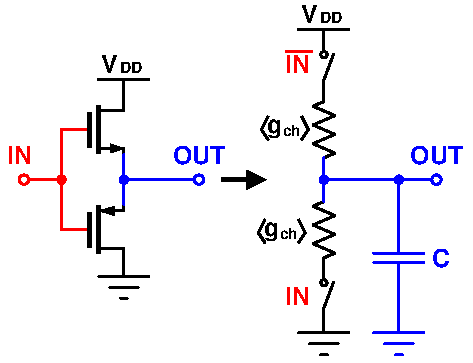
\includegraphics[width=\linewidth]{figs/design/inv_rc_model}
	            \caption{Inverter approximate model.}
	            \label{fig:inv_cir}
	        \end{subfigure}%
	        \begin{subfigure}{.5\textwidth}
	            \centering
	            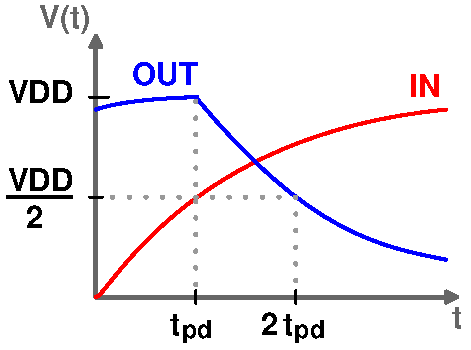
\includegraphics[width=0.8\linewidth]{figs/design/inv_waves}
	            \caption{Inverter waveforms in ring oscillator.}
	            \label{fig:inv_wave}
	        \end{subfigure}
	        \caption{Approximate model for ring oscillator inverter delay cell.}
	        \label{fig:inv_model}
	    \end{figure}

		To calculate oscillation frequency ring oscillator from the RC model, several inferences are made:
		\begin{itemize}
			\item The switching point $V_M$ of the inverters is $V_{DD}/2$, based on the assumption that the NMOS and PMOS are of equal strength.
			\item The output of an inverter will have a decaying exponential which starts coincident with the passing of $V_M$ at the input.
			\item The propagation delay $t_{pd}$ for an inverter will be the time differential between the $V_M$ crossing points on the input and output.
			\item The oscillator frequency will be $f_{osc}$ = $1/2Nt_{pd}$, where N is the number of stages (i.e. defined by 2N propagation delays).
		\end{itemize}
			Given the falling edge inverter waveform equation in \ref{eq:inv_exp}, and observing that $t_{pd}$ occurs at the point where $V(t) = V_{DD}/2$, it is found that $t_{pd}$ = $\tau\ln(2)$. Finally, using the aforementioned assumptions, the equation for oscillator frequency in equation \ref{eq:ro_osc_freq}.

			\begin{equation}\label{eq:inv_exp}
			V(t) = V_{DD}\cdot e^{\frac{-t}{\tau}}\cdot u(t)
			\end{equation}

			\begin{equation}\label{eq:ro_osc_freq}
				f_{osc}^{-1} = 2Nt_{pd} = \frac{2\ln(2)NC}{\langle g_{ch}\rangle}
			\end{equation}


		\subsubsection{Finding $\langle g_{ch}\rangle$ and C}
			The node capacitance C is trivial to find based on the inverter gate capacitance and a lumped load capacitance term $C_L$:
			\begin{equation}
				C = C_{ox}\left ( W_N L_N + W_P L_N \right) + C_L
			\end{equation}
			The average channel conductance $\langle g_{ch} \rangle$ is more involved to find. To do so, several assumptions are made:
			\begin{itemize}
				\item L $>>$ L$_{min}$, so no velocity saturation, and therefore square law is applicable.
				\item NMOS and PMOS have equal $V_{TH}$ and transconducance.
				\item Output transition occur with the active FET in saturation from the start of the transition until $t_{pd}$ after the start of the transition. This requires:
				\begin{itemize}
					\item $V_{DD}/4 < V_{TH} < V_{DD}/2$
				\end{itemize}
			\end{itemize}
			Following those assumptions, $\langle g_{ch} \rangle$ can be computed via integral within the period $t_{pd}$:
			\begin{equation}
				\langle g_{ch} \rangle = \frac{1}{t_{pd}} \int_0^{t_{pd}}\frac{I_{out}(t)}{V_{out}(t)}dt
			\end{equation}
			$I_{out}$ is computed using the saturated MOSFET square law model an exponential waveforms assumptions. An $I_{short}$ term is included to account for output current reduction from short-circuit conduction when both PMOS and NMOS are conducting.
			\begin{align}
				I_{out}(t) &= \frac{k_n}{2}\left(\frac{W}{L}\right)_n\left[\left(V_{in}(t) - V_{TH}\right)^2 \right]  - I_{short} \\
				&= \frac{k_n}{2}\left(\frac{W}{L}\right)_n \left[\left(V_{DD}\left(1-e^{-t/\tau}\right) - V_{TH}\right)^2 - \left(\frac{V_{DD}}{2} -V_{TH}\right)^2\right]
			\end{align}
			$k_n = \mu_nC_{ox}$, with the equal PMOS/NMOS assumption, $k_n\left(\frac{W}{L}\right)_n=k_p\left(\frac{W}{L}\right)_p$. $V_{out}$ is simply a decaying exponential with a delay $t_{pd}$ versus the input:
			\begin{equation}
				V_{out} = V_{DD}e^{-(t-t_{pd})/\tau}
			\end{equation}
			Now, computing the integral for $\langle g_{ch} \rangle$ yields:
			\begin{equation}
				\langle g_{ch} \rangle = \frac{1}{2}\mu_nC_{ox}\left(\frac{W}{L}\right)_n\left[V_{DD}\left(\frac{7}{8\ln2}-1\right)-V_{TH}\left(\frac{1}{\ln2}-1\right) \right]
			\end{equation}
			As a simplification, $\alpha$ is defined as:
			\begin{equation}
				\alpha = \left[V_{DD}\left(\frac{7}{8\ln2}-1\right)-V_{TH}\left(\frac{1}{\ln2}-1\right) \right]
			\end{equation}	
		
		\subsubsection{Handling unequal NMOS/PMOS}
			In the case of different threshold voltages for NMOS and PMOS:
			\begin{equation}
				f_{osc}^{-1} = N(t_{pdn} + t_{pdp}) = \ln(2)NC\left(\frac{1}{\langle g_{ch}\rangle_n} + \frac{1}{\langle g_{ch}\rangle_p}\right) = \frac{2\ln(2)NC}{\langle g_{ch}\rangle'}
			\end{equation}	
			A modified $\langle g_{ch}\rangle'$ is defined:
			\begin{align}
				\langle g_{ch}\rangle' = 2\left(\frac{1}{\langle g_{ch}\rangle_n} + \frac{1}{\langle g_{ch}\rangle_p}\right)^{-1} = 2\frac{\langle g_{ch}\rangle_n \langle g_{ch}\rangle_p}{\langle g_{ch}\rangle_n + \langle g_{ch}\rangle_p}
				= 2\frac{\frac{1}{2}\mu_nC_{ox}\left(\frac{W}{L}\right)_n \alpha_n\frac{1}{2}\mu_pC_{ox}\left(\frac{W}{L}\right)_p \alpha_p}{\frac{1}{2}\mu_nC_{ox}\left(\frac{W}{L}\right)_n\alpha_n + \frac{1}{2}\mu_pC_{ox}\left(\frac{W}{L}\right)_p\alpha_p}
			\end{align}	
			This is somewhat unmanagable, however enforcing $\mu_nC_{ox}\left(\frac{W}{L}\right)_n = \mu_pC_{ox}\left(\frac{W}{L}\right)_p$ for $V_M$ to equal $V_{DD}/2$ gives:
			\begin{align}
				\langle g_{ch}\rangle' = \frac{1}{2}\mu_nC_{ox}\left(\frac{W}{L}\right)_n\frac{2 \alpha_n\alpha_p}{\alpha_n + \alpha_p} = \frac{1}{2}\mu_nC_{ox}\left(\frac{W}{L}\right)_n \alpha'
			\end{align}	
			Thus $\alpha_n$ and $\alpha_p$ are found for the according threshold voltages and then $\langle g_{ch}\rangle$ can be found.
			\begin{equation}
				\alpha' =  \frac{2 \alpha_n\alpha_p}{\alpha_n + \alpha_p}
			\end{equation}

		\subsubsection{Solving for oscillator frequency and power}
			Solving for oscillator frequency:
			\begin{equation}
				f_{osc} = \frac{\mu_nC_{ox}}{4\ln2NC}\left(\frac{W}{L}\right)_n\left[V_{DD}\left(\frac{7}{8\ln2}-1\right)-V_{TH}\left(\frac{1}{\ln2}-1\right) \right]
			\end{equation}
			If gate capacitance is the dominant load component, and PMOS/NMOS are equal sized such that $C=2WLC_{ox}$:
			\begin{equation}
				f_{osc} = \frac{\mu_n}{8\ln2N}\cdot\frac{1}{L^2}\left[V_{DD}\left(\frac{7}{8\ln2}-1\right)-V_{TH}\left(\frac{1}{\ln2}-1\right) \right]
			\end{equation}
			Power can also be calculated, knowing in digital circuits $P = fC_{\Sigma}V_{DD}^2$, where $C_{\Sigma}$ is the total capacitance of the active nodes. Thus:
			\begin{equation}
				P_{osc} = Nf_{osc}CV_{DD}^2 = \frac{\mu_nC_{ox}}{4\ln2}\left(\frac{W}{L}\right)_n\left[V_{DD}\left(\frac{7}{8\ln2}-1\right)-V_{TH}\left(\frac{1}{\ln2}-1\right) \right]
			\end{equation}
			It should be noted that the power consumption is proportional to FET aspect ratio (W/L), regardless of the load.

	\subsubsection{Ring oscillator backgate tuning derivation}
		Using the basic expressions for ring oscillator frequency, the operature under backgate biasing can be found. In FD-SOI, the threshold voltage of a FET varies with linear dependence on the applied back gate bias $V_{BG}$ (relative to source). Given the body effect coefficient of a process, $\gamma$, $V_t$ is:
		\begin{equation}
			V_{TH} = V_{t0} - \gamma V_{BG}
		\end{equation}
		Using this in the ring oscillator frequency equation:
		\begin{equation}
			f_{osc} = \frac{\mu_nC_{ox}}{4\ln2NC}\left(\frac{W}{L}\right)_n\left[V_{DD}\left(\frac{7}{8\ln2}-1\right)-V_{t0}\left(\frac{1}{\ln2}-1\right) + \gamma V_{BG}\left(\frac{1}{\ln2}-1\right) \right]
		\end{equation}
		Equivalently, $f_{osc} = f_{0,osc} + \Delta f_{osc}(V_{BG})$, provided $f_{0,osc}$ is the frequency with no backgate bias where. Thus it is found that:
		\begin{equation}\label{eq:kvco_}
			\Delta f_{osc}(V_{BG}) = \gamma V_{BG}\frac{\mu_nC_{ox}}{4\ln2NC}\left(\frac{W}{L}\right)_n\left[\frac{1}{\ln2}-1\right] = K_{VCO}
		\end{equation}	

		The important finding here is that the change in oscillator frequency is linear with backgate voltage, that is $\Delta f_{osc} \propto V_{BG}$. The expression of \ref{eq:kvco_} also happens to to be the oscillator VCO gain, $K_{VCO}$. Given the wide voltage range that FD-SOI backgates may be biased to, this implies that a highly linear VCO with wide input range may be implemented with backgate tuning. If the backgate voltage is constrained in the range [0, $V_{DD}$], the center frequency $f_c$ of such a VCO is then:
		\begin{equation}
			f_{c} = \frac{\mu_nC_{ox}}{4\ln2NC}\left(\frac{W}{L}\right)_n\left[V_{DD}\left(\frac{7}{8\ln2}-1+\frac{\gamma}{2\ln2}-\frac{\gamma}{2}\right)-V_{t0}\left(\frac{1}{\ln2}-1\right)\right]
		\end{equation}
		Correspondingly, the tuning range with $V_{BG} \in$ [0, $V_{DD}$] is:
		\begin{equation}\label{eq:tuning_range}
			\Delta f = \gamma V_{DD}\frac{\mu_nC_{ox}}{4\ln2NC}\left(\frac{W}{L}\right)_n\left[\frac{1}{\ln2}-1\right]
		\end{equation}
		Finally, the fractional tuning range of the oscillator found to be that of equation \ref{eq:frac_range}. Notice that this is only a function of supply voltage $V_{DD}$, nominal threshold voltage $V_{t0}$ and body effect coefficient $\gamma$.
		\begin{equation}\label{eq:frac_range}
			\frac{\Delta f}{f_c} = \frac{\gamma V_{DD}\left( 1-\ln2 \right)}{V_{DD}\left(\frac{7}{8}-\ln2+\frac{\gamma}{2}-\frac{\gamma}{2}\ln2\right)-V_{t0}\left(1-\ln2\right)}
		\end{equation}	
		If a N-bit DAC is used to control the oscillator, the resulting DCO gain is therefore:
		\begin{equation}
			K_{DCO} = \frac{\Delta f}{2^{N_{DAC}}} = \frac{f_c}{2^{N_{DAC}}}\cdot\frac{\gamma V_{DD}\left( 1-\ln2 \right)}{V_{DD}\left(\frac{7}{8}-\ln2+\frac{\gamma}{2}-\frac{\gamma}{2}\ln2\right)-V_{t0}\left(1-\ln2\right)}
		\end{equation}	
	\subsubsection{DCO Gain Uncertainty}
		The DCO gain $K_{DCO}$ is used in setting the loop filter coefficients, so the uncertainty of the DCO gain is of interest to allow for statistical analysis of the PLL across process variation. The uncertainty of $K_{DCO}$ (normalized with nominal $K_{DCO}$ value) as a function of $V_{DD}$, $V_{t0}$ and $\gamma$ is:
		\begin{equation}
			\sigma_{KDCO} = \sqrt{\left(\frac{\partial K_{DCO}}{\partial V_{DD}}\cdot\frac{\sigma_{VDD}}{K_{DCO}} \right)^2 + \left(\frac{\partial K_{DCO}}{\partial V_{t0}}\cdot\frac{\sigma_{Vt0}}{K_{DCO}} \right)^2 + \left(\frac{\partial K_{DCO}}{\partial \gamma}\cdot\frac{\sigma_\gamma}{K_{DCO}} \right)^2}
		\end{equation}

		\begin{align}
			\frac{\partial K_{DCO}}{\partial V_{DD}} &= \frac{f_c}{2^{N_{DAC}+1}}\cdot\frac{-\gamma V_{t0}(1-\ln2)^2}{\left[ V_{DD}\left(\frac{7}{8}-\ln2+\frac{\gamma}{2}-\frac{\gamma}{2}\ln2\right)-V_{t0}\left(1-\ln2\right) \right]^2}\\
			\frac{\partial K_{DCO}}{\partial V_{t0}} &= \frac{f_c}{2^{N_{DAC}+1}}\cdot\frac{\gamma V_{DD}(1-\ln2)^2}{\left[ V_{DD}\left(\frac{7}{8}-\ln2+\frac{\gamma}{2}-\frac{\gamma}{2}\ln2\right)-V_{t0}\left(1-\ln2\right) \right]^2}\\
			\frac{\partial K_{DCO}}{\partial \gamma} &= \frac{f_c}{2^{N_{DAC}+1}}\cdot\frac{V_{DD}\cdot(1-\ln2) \left[ V_{DD}\left(\frac{7}{8}-\ln2\right)-V_{t0}\left(1-\ln2\right) \right]}{\left[ V_{DD}\left(\frac{7}{8}-\ln2+\frac{\gamma}{2}-\frac{\gamma}{2}\ln2\right)-V_{t0}\left(1-\ln2\right) \right]^2}
		\end{align}
		Simplified:
		\begin{multline}
			\sigma_{KDCO} = \frac{1}{\gamma V_{DD} \left[ V_{DD}\left(\frac{7}{8}-\ln2+\frac{\gamma}{2}-\frac{\gamma}{2}\ln2\right)-V_{t0}\left(1-\ln2\right) \right]}\cdot\\ \sqrt{\left(\gamma V_{t0} (1-\ln2)\sigma_{VDD} \right)^2 + \left(\gamma V_{DD} (1-\ln2)\sigma_{Vt0} \right)^2 + \left( V_{DD}\left[ V_{DD}\left(\frac{7}{8}-\ln2\right)-V_{t0}\left(1-\ln2\right) \right]\sigma_{\gamma} \right)^2 }
		\end{multline}	

		% \hl{Motivate selection of fine backgate tuning and supply coarse tuning (as future extension?). I.e. what is df/dVdd vs df/dVbg?}
		% \hl{\textbf{TODO} - extract $\gamma$, $V_{t0}$ variance for FETs in process kit, place in results?}

		\subsubsection{Backgate-controlled Ring Oscillator Sensitivity Analysis}
		The frequency tuning sensitivity of the ring oscillator for supply and backgate voltages will be compared. First the following is defined, following that the derived equations for oscillator frequency are linear.
		\begin{equation}
			f_{osc}(V_{DD}+\Delta V_{DD}) = f_{osc}(V_{DD}) + f_{osc}(\Delta V_{DD})
		\end{equation}
		\begin{equation}
			f_{osc}(V_{DD}) = f_0
		\end{equation}
		\begin{equation}
			f_{osc}(\Delta V_{DD}) = \Delta f
		\end{equation}

		In the case of supply voltage tuning, the change (proportion) of frequency per voltage of applied extra bias is (evaluated at zero back-gate bias):
		\begin{equation}
			S^{f_{osc}}_{V_{DD}} = \frac{\Delta f}{f_0}\cdot\frac{1}{\Delta V_{DD}}  = \frac{\left(\frac{7}{8\ln2}-1\right)}{V_{DD}\left(\frac{7}{8\ln2}-1\right)-V_{t0}\left(\frac{1}{\ln2}-1\right)}
		\end{equation}
		With $V_{DD}$ = 0.8, $V_{t0}$ = 0.3 (approximately true for 22FDX devices), it is expected 340\% change in frequency will result per extra volt of applied bias. Of course, this is linearized, and one does not expect to apply an extra 1V of supply bias to a 0.8V oscillator. Realistically, the supply can be tuned $\pm$ 10\%, which corresponds to a $\pm$27.2\% tuning range of the oscillator. Supply tuning stands as a viable coarse tuning mechanism for the oscillator, however, fine tuning is more limited due to difficulty in achieving small resolution step (e.g 10 bits in $V_{DD}$ = 0.8V $\pm$10\% corresponds to 156 $\mu$V/LSB, and 26 m\%/LSB of frequency tuning).

		\par In the case of backgate tuning, the change (proportion) of frequency per volt of applied backgate bias is:
		\begin{equation}
			S^{f_{osc}}_{V_{BG}} = \frac{\Delta f}{f_0}\cdot\frac{1}{\Delta V_{BG}}  = \frac{\gamma \left(\frac{1}{\ln2}-1\right)}{V_{DD}\left(\frac{7}{8\ln2}-1\right)-V_{t0}\left(\frac{1}{\ln2}-1\right)}
		\end{equation}

		With $\gamma$=0.07, $V_{DD}$=0.8, $V_{t0}$=0.3, as is typical in 22FDX, it is expected a 29.5\% change in frequency will result per volt applied of backgate bias. This is much finer than achieved with supply voltage tuning. The ratio of frequency sensitivity to supply and backgate voltage tuning is:

		\begin{equation}
			\frac{S^{f_{osc}}_{V_{DD}}}{S^{f_{osc}}_{V_{BG}}} =  \frac{\frac{7}{8\ln2}-1}{\gamma \left(\frac{1}{\ln2}-1\right)}
		\end{equation}
		Under the aforementioned biasing conditions, it is expected that 8.4x finer control can be achieved with backgate tuning. The wide backgate voltage ranges allowed for with FD-SOI technology permit for design of a voltage-DAC based controll scheme which will achieve far smaller frequency resolution than with supply voltage tuning. 

		\subsubsection{Capacitor-based coase tuning scheme}
		It is observed that oscillator frequency of ring oscillator is capacitance dependent. Thus if a bank of quantized capacitances may be switched into the oscillator, coarse control of frequecy can be implemented. Figure \ref{fig:rosc_tuning} demonstrates the effect of such a tuning scheme, for increasing capacitance settings C0-C3. Under such a scheme it is important to ensure that the frequency ranges acheived through backgate tuning overlap between sucessive capacitor settings to ensure continuity of frequencies accessible by the oscillator. 
		\FloatBarrier
		\begin{figure}[htb!]
			\center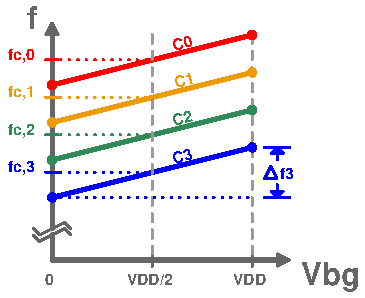
\includegraphics[width=0.4\linewidth, angle=0]{figs/backgate_rosc_tuning2.pdf}
			\caption{Backgate-tuned ring oscillator with coarse tuning capacitor bank.}
			\label{fig:rosc_tuning}
		\end{figure}

%%%%%%%%%%%%%%%%%%%%%%%%%%%%%%%
		
		\FloatBarrier\pagebreak
		\subsubsection{Pseudodifferential Backgate-Coupled Inverter Delay Cell}\label{sec:pd_inv}
		To utilize backgate tuning for frequency control, a suitable delay cell design must be devised. Accordingly, the delay topology used in this work has been derived from the FD-SOI pseudodifferential backgate coupled inverter delay cell of \cite{Jacquemod2019}, shown in figure \ref{fig:bg_inv_jacqu}. This inverter uses two single ended FD-SOI inverters, with the backgates of the transistors in a given inverter connected together. This is implemented with a common well structure below the two transistors of each inverter. Nominally, to avoid forward biasing of the well-substrate diodes, a N-doped well or a triple well is used, with well potentials constrained to be $\geq$ 0. The result of this well configuration and the FD-SOI BOX layer is that the backgate terminals of the PMOS and NMOS may be tuned in tandem across a wide positive voltage range. This is not possible in bulk technology. In 22FDX, such well configurations allow biasing from 0 to +2V, which is inclusive of the full rail-to-rail range of a circuit supplied with $V_{DD}$ = 0.8V, as in this work. Thus, in figure \ref{fig:bg_inv_jacqu}, when the two FD-SOI sub-cells inverter cells connected with the shown cross-coupled output and backgate configuration, safe well biasing is achieved. The backgate cross-coupled configuration has the effect of inducing differential behavior in the circuit, as positive feedback is introduced. It should be noted that cell of figure \ref{fig:bg_inv_jacqu} does not employ back gate tuning to tune frequency. This work proposes a modification to the topology which implements backgate differential coupling and backgate frequency tuning.

		\begin{figure}[htb!]
		        \centering
		        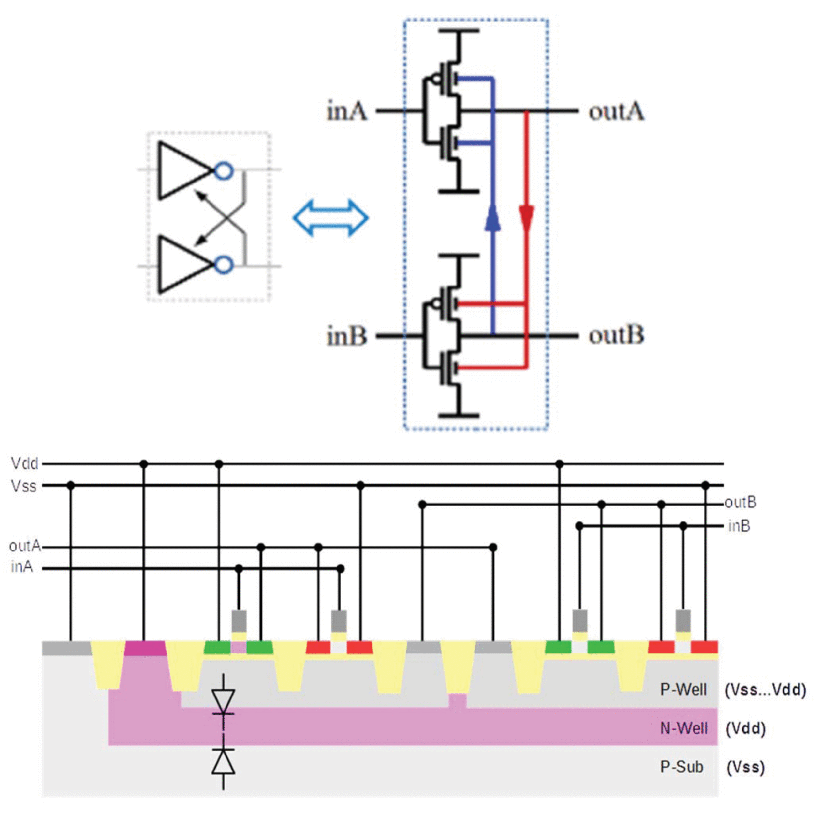
\includegraphics[width=0.58\textwidth, angle=0]{./figs/design/jacqu2-1-large.png}
		    \caption{FD-SOI backgate-coupled inverter topology, .}
		    \label{fig:bg_inv_jacqu}
		\end{figure}	

		The emergence of differential behavior in this delay cell can be understood through circuit analysis. First, the common backgate inverter cell (figure \ref{fig:fig_10a}) is converted to a linearized model, for an arbitrary bias point, in figure \ref{fig:fig_10b}. A simplification of the linearized model is arrived at by lumping terms together, giving figure \ref{fig:fig_10c}. Using the linearized model of figure \ref{fig:fig_10c}, a linearized version of the pseudodifferential inverter circuit is then arrived at in figures \ref{fig:pseudodiff_cir} and \ref{fig:pseudodiff_linearized}. It is observed that transconductors $-G_{mb}$ in figure \ref{fig:pseudodiff_linearized} couple the two outputs with positive feedback loop. Therefore, any differential components generated via the feed forward terms $-G_m R_o v_{in}$ and $-G_m R_o v_{ip}$ will be positively amplified by the cross coupling. Elementary circuit analysis for differential gain of the linear circuit in figure \ref{fig:pseudodiff_linearized} leads to the expression in equation \ref{eq:pd_dm_gain}.

			\begin{figure}[htb!]
			    \centering
			    \begin{subfigure}{0.33\textwidth}
			        \centering
			        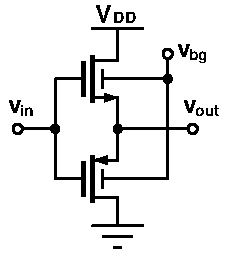
\includegraphics[width=1\textwidth, angle=0]{./figs/design/fig_10a_}
			        \caption{ }
			        \label{fig:fig_10a}
			    \end{subfigure}%
			    \begin{subfigure}{0.33\textwidth}
			        \centering
			        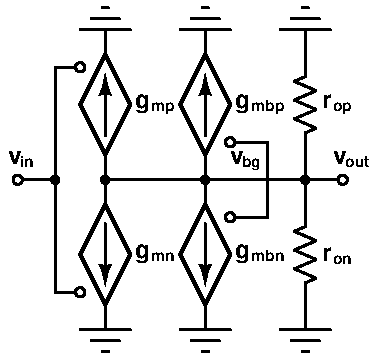
\includegraphics[width=1\textwidth, angle=0]{./figs/design/fig_10b}
			        \caption{ }
			        \label{fig:fig_10b}
			    \end{subfigure}
			    \begin{subfigure}{0.33\textwidth}
			        \centering
			        \includegraphics[width=1\textwidth, angle=0]{./figs/design/fig_10c}
			        \caption{ }
			        \label{fig:fig_10c}
			    \end{subfigure}
			    % \caption{x.}
			    \caption{\textbf{(a)} Common backgate inverter, \textbf{(b)} Linearized circuit, \textbf{(c)} Simplified linearized model.}
			    \label{fig:bg_inv_model}
			\end{figure} 

			\begin{figure}[htb!]
			    \centering
			    \begin{subfigure}{0.3\textwidth}
			        \centering
			        \includegraphics[width=1\textwidth, angle=0]{./figs/design/pseudodiff_bw}
			        \caption{ }
			        \label{fig:pseudodiff_cir}
			    \end{subfigure}%
			    \hspace{5em}
			    \begin{subfigure}{0.35\textwidth}
			        \centering
			        \includegraphics[width=1\textwidth, angle=0]{./figs/design/pseudodiff_buff_linear}
			        \caption{ }
			        \label{fig:pseudodiff_linearized}
			    \end{subfigure}
			    % \caption{x.}
			    \caption{\textbf{(a)} Pseudodifferential backgate-coupled inverter circuit, \textbf{(b)} Linearized circuit.}
			    \label{fig:pd_cir_inv_model}
			\end{figure} 

			\begin{equation}\label{eq:pd_dm_gain}
				A_{DM} = \frac{G_mR_o + G_{mb}^2R_o^2}{1 - G_{mb}^2R_o^2}
			\end{equation}
			Using the relation $G_{mb} = \gamma G_{m}$ found in equation \ref{eq:gm_gmb_relation}, equation \ref{eq:pd_dm_gain} can be simplified to \ref{eq:pd_dm_gain2} (this is assuming PMOS and NMOS have approximately equal $\gamma$). In the special case where $\gamma G_mR_o \approx 1$, the differential gain of the delay cell can be very high, implying the pseudodifferential coupling can be very effective at inducing differential behavior. A major advantage of this topology is that it is implemented using only two inverters, unlike typical differential pair circuits which rely on current biasing to achieve differential behavior. The removal of the need for current biasing reduces power consumption, as no bias generators are required. Circuit noise is also reduced due to fewer total transistors generating noise in the circuit.
			\begin{equation}\label{eq:pd_dm_gain2}
				A_{DM} = \frac{G_mR_o }{1 - \gamma G_mR_o }
			\end{equation}
			For the sake of completeness, the common mode gain of the circuit has also been determined by the same method, given in equation \ref{eq:pd_cm_gain}.
			\begin{equation}\label{eq:pd_cm_gain}
				A_{CM} = \frac{G_mR_o }{1 + \gamma G_mR_o }
			\end{equation}

%%%%%%%%%%%%%%%%%%%%%%%%%%%%%%%%%%%%%%%%%%%%%%%%%%%%%%%%%%%%%%%%%%%%%%%%%%%

			\FloatBarrier\subsubsection{Tunable Frequency Backgate-Coupled Pseudodifferential Delay Cell}
			To implement the backgate-coupled pseudo-differential inverter delay cell topology with backgate tuning, two cantidate topologies have been devised. The first is the parallel cofigured topology of figure \ref{fig:parallel_delay_cell}, and the second is a telescopic configutation, shown in figure \ref{fig:telescopic_delay_cell}.

			\begin{figure}[htb!]
			    \centering
			    \begin{subfigure}{0.5\textwidth}
			        \centering
			        \includegraphics[width=1\textwidth, angle=0]{./figs/design/parallel_delay_cell2}
			        \caption{ }
			        \label{fig:parallel_delay_cell}
			    \end{subfigure}%
			    \begin{subfigure}{0.5\textwidth}
			        \centering
			        \includegraphics[height=0.5\textheight, angle=0]{./figs/design/tele_delay_cell2}
			        \caption{ }
			        \label{fig:telescopic_delay_cell}
			    \end{subfigure}
			    % \caption{x.}
			    \label{fig:tunable_delay_cells}
			    \caption{Backgate tunable backgate-coupled pseudodifferential delay cell in\textbf{(a)} Parallel, \textbf{(b)} Telescopic implementations.}
			\end{figure} 


			The parallel cofigured topology employs backgate-coupled pseudo-differential inverter in parallel with a second set of inverters, which the backgate voltages are set externally to control the oscillator frequency. 


			The telecopic topology is comprised of two sub-inverters each with a telescopic stack of four transistors. The header and footer transistor backgates are connected to external control voltages to adjust frequency. Modulating the control voltages will modulate the conductance of the header and footer devices, which result in a current-starving like behavior that modulate oscillator frequency. The inner pair of transistors in each sub-inverter are configured with a common backgate, which are cross-coupled with the output of the other respective sub-inverter, to induce differential operation in the same manner as the basic backgate-coupled pseudo-differential inverter delay cell. 

			Hajimiri's oscillator impulse sensitivity function (ISF) paper \cite{Hajimiri1998} suggests that it is favorable for an oscillator to have as symmetric rise and fall time. Higher symmetry of waveform results in a lower corner frequency for flicker noise, thus low frequency phase noise will be improved.



			\begin{figure}[htb!]
			    \centering
			    \includegraphics[width=0.4\textwidth, angle=0]{./figs/design/tuning}
			    \caption{Complementary tuning of backgate voltages to achieve frequency tuning.}
			    \label{fig:bg_tuning_scheme}
			\end{figure}



			\begin{itemize}[itemsep=4pt,label=\protect---]
				\item Must use devices in N well (PFET, HVTPFET, SLVTNFET, LVTNFET) to not forward bias substrate diode.
				\item To achieve $V_{m}$ =  $V_{DD}/2$, PFET + LVTNFET give most reasonable W$_P$/W$_N$, ca 1.2-1.4.
				\begin{itemize}[itemsep=4pt,label=$\bullet$]
					\item SLVTNFET + PFET needs W$_P$/W$_N$ $\approx$ 8.
				\end{itemize}
			\end{itemize}


			\begin{figure}[htb!]
			    \centering
			    \begin{subfigure}{0.5\textwidth}
			        \centering
			        \includegraphics[width=1\textwidth, angle=0]{./figs/design/ratio_lvtnfet_pfet}
			        \caption{ }
			        \label{fig:ratio_lvtn_p}
			    \end{subfigure}%
			    \begin{subfigure}{0.5\textwidth}
			        \centering
			        \includegraphics[width=1\textwidth, angle=0]{./figs/design/ratio_slvtnfet_pfet}
			        \caption{ }
			        \label{fig:ratio_slvtn_p}
			    \end{subfigure}
			    % \caption{x.}
			    \label{fig:opt_ratio}
			    \caption{\textbf{(a)} Optimal width PFET/LVTNFET, \textbf{(b)} Optimal width PFET/SLVTNFET.}
			\end{figure} 


			\begin{itemize}[itemsep=4pt,label=\protect---]
				\item Good symmetry of rise time observed, with $V_{cm}$ close to $V_{DD}/2$ over the full oscillation cycle.
				\item \textbf{Observed 10.3\% fractional frequency tuning with L=150nm, FOM=-161 dB, 1:1 ratio of inverters.}
				\item I require $<$ 1\% fractional tuning range to achieve my $K_{DCO}$ with a 10b DAC, this will not work. The (W/L) becomes large to achieve a high inverter ratio, thus increases power too much.
			\end{itemize}



			\begin{itemize}[itemsep=4pt,label=\protect---]
				\item Modify the pseudo-differential cell to have header/footer transistors with back gate control.
				\begin{itemize}[itemsep=4pt,label=$\bullet$]
					\item Cross-coupled devices force differential operation
					\item Header/footer devices used to adjust frequency.
				\end{itemize}				
				\item Ratioing the size of the header/footer devices to the size of the cross-coupling devices tunes $K_{VCO}$
				\item \textbf{Requires complementary control of backgate voltage for tuning.}
			\end{itemize}



			\begin{itemize}[itemsep=4pt,label=\protect---]
				\item Good symmetry of rise time observed, with $V_{cm}$ close to $V_{DD}/2$ over the full oscillation cycle.
				\item $W_p$/$W_n$ = 1.25. Nominal (W/N)$_n$ = 400n/150n
				\item \textbf{1:1 ratioing: Observed 10.0\% fractional frequency tuning with L=150nm, {\color{red}FOM=-162.6 dB.}}
				\item \textbf{1:2 ratioing (header/footer larger): Observed 4.8\% fractional frequency tuning with L=150nm.}
				\item Still hard to get required $<$ 1\% fractional frequency tuning.
			\end{itemize}

			% \begin{figure}[htb!]
			%         \centering
			%         \includegraphics[width=0.8\textwidth, angle=0]{./figs/telescopic_wfm}
			%     % \caption{Approximate model for ring oscillator inverter delay cell.}
			% \end{figure}



			\begin{itemize}[itemsep=4pt,label=\protect---]
				\item Not as linear as I had hoped, $K_{VCO}$ decreases by -33\% when $V_{DD}$ is swept [0, 0.8] V.
				\item I have observed a decease in $\gamma$ at higher back gate biases, this and mobility degredation(??) might explain this trend.
			\end{itemize}



			% \vspace{100em}
			\begin{itemize}[itemsep=4pt,label=\protect---]
				\item PVT (coarse), medium and fine tuning all need to coexist (overlap in frequency).
				\item PVT tuning achieved with bank of differentially connected capacitors
				\item Fine/medium tuning achieved with parallel combination of header/footer transistors. The ratio of these devices affects the difference of the ranges.

			\end{itemize}


			\begin{figure}[htb!]
			        \centering
			        \includegraphics[height=0.6\textheight, angle=0]{./figs/design/delay_cell_pd_inv}
			    \caption{Backgate coupled pseudo-differential inverter delay cell with fine and medium tuning ranges.}
			    \label{fig:pd_delay_cell_fine_med}
			\end{figure}

			\begin{figure}[htb!]
			    \centering
			    \begin{subfigure}{0.5\textwidth}
			        \centering
			        \includegraphics[width=1\textwidth, angle=0]{./figs/results/osc_se_waves}
			        \caption{ }
			        \label{fig:osc_se_waves}
			    \end{subfigure}%
			    \begin{subfigure}{0.5\textwidth}
			        \centering
			        \includegraphics[width=1\textwidth, angle=0]{./figs/results/osc_cmv}
			        \caption{ }
			        \label{fig:osc_cmv}
			    \end{subfigure}
			    % \caption{x.}
			    \caption{\textbf{(a)} Oscillator single-ended waveforms, \textbf{(b)} Oscillator common mode voltage waveform.}
			    \label{fig:osc_waves}
			\end{figure} 


	 Could not get 2 quadrature oscillator stage to oscillate. Period is 4tpd, thus a transition occurs every 2tpd. Propogation delay is ln(2)tau, so a transition every 1.38tau, which equates to enough time to settle to 75\% of the final voltage. Because of partial settling, the oscillation dies in a couple cycles, and is not viable here. To achieve quadrature, 4 stages must be used, however, this was slow to acheive the target 2.448 GHz. Thus, use of sub-harmonic oscillator (show edge combining) due to speed limitations (need short channel length to get right speed, unfortunately phase noise degrades).

		\subsection{Full circuit}
			\begin{figure}[htb!]
			        \centering
			        \includegraphics[width=0.8\textwidth, angle=0]{./figs/design/ro_6st_simple}
			    \caption{Basic differential ring oscillator circuit.}
			    \label{fig:basic_6stg_ro}
			\end{figure}
			\begin{figure}[htb!]
			        \centering
			        \includegraphics[width=1.0\textwidth, angle=0]{./figs/design/ro_12ph_quad}
			    \caption{Third subharmonic to quadrature full rate conversion.}
			    \label{fig:ro_phases}
			\end{figure}

			\begin{figure}[htb!]
			        \centering
			        \includegraphics[width=0.5\textwidth, angle=0]{./figs/design/delay_cell_symbol_full}
			    \caption{Ring oscillator delay cell symbol.}
			    \label{fig:delay_cell_symbol}
			\end{figure}

			\begin{figure}[htb!]
			        \centering
			        \includegraphics[width=0.8\textwidth, angle=0]{./figs/design/delay_cell_full}
			    \caption{Ring oscillator delay cell full circuit.}
			    \label{fig:delay_cell_circuit}
			\end{figure}
			\begin{figure}[htb!]
			        \centering
			        \includegraphics[width=1.5\textwidth, angle=90]{./figs/design/rosc_full_6stg}
			    \caption{Ring oscillator full schematic.}
			    \label{fig:full_6sg_ro}
			\end{figure}


	 Compare RO model (back gate linearity, VDD tuning) to data. There is agreement.
		\subsubsection{Layout}








% ################################################################################################
% ################################################################################################
	\pagebreak\FloatBarrier
	\subsection{Loop Filter}
	For selection of a loop filter, some basic criteria have been selected for desirable synthesizer behavior:
	\begin{enumerate}[itemsep=0pt,label=\protect\mycirc{\arabic*}]
		\setlength\itemsep{-0.8em}
		\item Zero steady state error, for accuracy of the synthesized frequency.
		\item Minimize complexity of implemented logic (i.e. minimize the number of loop filter poles and zeros).
		\item Low pass response of PLL in closed-loop.
	\end{enumerate}
	From this author's previous work \cite{Me}, it was established that the pole-zero filter satisfying these requirements is a proportional-integral controller.

\subsubsection{Proportional-integral Loop Filter}
 A proportional-integral controller \cite{ogata_2010_pid} is given in equation \ref{eq:pi_pll_tf}, containing an proportional gain term $K_p$, and an integral gain term $K_p$. This can be optionally represented using a pole at zero and a zero with $\omega_z = K_i/K_p$:
			\begin{equation} \label{eq:pi_pll_tf}
				\textnormal{H}_{LF}(s) = K_p + \frac{K_i}{s}  = \frac{K_i}{s}\left(\frac{s}{\omega_z} + 1\right) 
			\end{equation}
			Substitution of this controller into the PLL closed loop transfer function (equation \ref{eq:cont_pll_tf2}) results in:
			\begin{equation}\label{eq:pi_bbpdpll_tf}
				T(s) = \frac{\Phi_{out}(s)}{\Phi_{ref}(s)} =  \frac{ 2\pi K_{BBPD}K_{DCO}K_{i} \left(\frac{s}{\omega_z} + 1\right) }{s^2 + 2\pi K_{BBPD}K_{DCO}K_{i}\left(\frac{s}{\omega_z} + 1\right) }
			\end{equation}

	\subsubsection{Discretization of Loop Filter}\label{disc_lf_comp_pi}
		Using the continuous filter discretization approach described in section \ref{lf-discretization} on the loop filter of equation \ref{eq:pi_pll_tf} results in equation \ref{eq:z_lf}. When converting a continuous time PLL model into a discrete time controller implementation, a commonly cited rule of thumb in PLL literature states that the PLL loop bandwidth should be contstrained as $BW_{loop} \leq$  0.1$f_{ref}$ \cite{gardner_1980} (here $\Delta T_s = 1/f_{ref}$). This is due to the fact that low degrees of oversampling lead to deviations between continuous PLL models and real sampled-PLL performance, possibly causing instability or sub-optimal performance versus an intended design.
		\begin{align}
			\textnormal{H}_{LF}(z) & = \left.\frac{K_i}{s}\left(\frac{s}{\omega_z} + 1\right)\right\vert_{s=\frac{1}{\Delta T_s}(1-z^{-1})}
			&= K_p\frac{(1+\omega_z\Delta T_s)-z^{-1}}{1- z^{-2}}\label{eq:z_lf}
		\end{align}

		The transformation of equation \ref{eq:z_lf} into a digitally implementable design as a direct form 1 IIR filter shown in figure \ref{fig:filt_imple}. Its filter coefficients given by equations \ref{eq:b0_coef} and \ref{eq:b1_coef}.
		\begin{figure}[htb!]
			\center\fontfamily{\sfdefault}\selectfont
% XCircuit output "filter_arch_pi.tex" for LaTeX input from filter_arch_pi.ps
\def\putbox#1#2#3#4{\makebox[0.00000in][l]{\makebox[#1][l]{}\raisebox{\baselineskip}[0.00000in][0.00000in]{\raisebox{#2}[0.00000in][0.00000in]{\scalebox{#3}{#4}}}}}
\def\rightbox#1{\makebox[0.00000in][r]{#1}}
\def\centbox#1{\makebox[0.00000in]{#1}}
\def\topbox#1{\raisebox{-0.60\baselineskip}[0.00000in][0.00000in]{#1}}
\def\midbox#1{\raisebox{-0.20\baselineskip}[0.00000in][0.00000in]{#1}}
   \scalebox{1}{
   \normalsize
   \parbox{5.54167in}{
   \includegraphics[scale=0.70000]{./figs/filter_arch_pi.pdf}\\
   % translate x=1728 y=944 scale 0.38
   \putbox{1.91800in}{0.90300in}{0.96}{$\frac{1}{\frac{s}{\omega_p} + 1}$}%
   \putbox{1.14800in}{1.01500in}{0.96}{$K_p$}%
   \putbox{1.14800in}{0.72800in}{0.96}{$K_i$}%
   \putbox{0.60900in}{0.58100in}{0.96}{$1/s$}%
   \putbox{0.25900in}{0.98700in}{0.96}{x[n]}%
   \putbox{2.35900in}{0.98700in}{0.96}{y[n]}%
   \putbox{2.92600in}{1.10600in}{0.96}{x[n]}%
   \putbox{4.99800in}{1.01500in}{0.96}{\rotatebox{-360}{y[n]}}%
   \putbox{3.26200in}{0.75600in}{0.96}{$z^{-1}$}%
   \putbox{3.73100in}{1.13400in}{0.96}{b$_0$}%
   \putbox{3.73100in}{0.66500in}{0.96}{b$_1$}%
   \putbox{4.83700in}{0.75600in}{0.96}{$z^{-1}$}%
   \putbox{4.99800in}{0.55300in}{0.96}{y[n-1]}%
   } % close 'parbox'
   } % close 'scalebox'
   \vspace{-\baselineskip} % this is not necessary, but looks better
\fontfamily{\rmdefault}\selectfont

			\caption{Implementation of filter.}
			\label{fig:filt_imple}
		\end{figure}

		\begin{align}
			b_0 &= K_p (1+\omega_z\Delta T_s) \label{eq:b0_coef}\\
			 b_1 &= -K_p \label{eq:b1_coef}
		\end{align}

\subsubsection{Optimal Filter Selection (Noisy BBPD)}
			Optimization of a loop filter under BBPD operation will be performed by minimizing the total integrated phase noise power out of the PLL. First, some mathematical simplifications of the PLL model are introduced. Rewriting equation \ref{eq:pi_bbpdpll_tf} with substitutions $\omega_z = K_i/K_p$ and $\mathrm{K} = 2\pi K_{BBPD}K_{DCO}K_{i}$:
			\begin{equation} \label{eq:simp_pi_pll_tf}
				T(s) = \frac{\Phi_{out}(s)}{\Phi_{ref}(s)} = \frac{s\frac{K}{\omega_z} + K }{s^2 + s\frac{K}{\omega_z} + K}
			\end{equation}
			The denominator can be redefined in terms of a natural frequency $\omega_n$ and damping ratio $\zeta$:
			\begin{equation}
				s^2 + s\frac{K}{\omega_z} + K = s^2 + s2\zeta\omega_n + \omega_n^2
			\end{equation}
			Thus, $\omega_n = \sqrt{K}$, and $\omega_z = \sqrt{K}/2\zeta$. The poles of equation \ref{eq:simp_pi_pll_tf} are then located at s = $\zeta\sqrt{K} \pm j\sqrt{K}\sqrt{1-\zeta^2}$. The time constant of the PLL is obtained from the real portion of the dominant pole in equation \ref{eq:simp_pi_pll_tf}:
			\begin{equation}
				\tau = \frac{1}{|\min(\Re(\{s_{p1}, s_{p2}\}))|}
			\end{equation}
			 It is of interest to minimize settling time of the PLL (i.e. time constant), thus maximizing the frequency of the dominant pole of the PLL is of interest. In the pole-zero plot of figure \ref{fig:pi_pll_pz}, the dominant pole of equation \ref{eq:simp_pi_pll_tf} is observed to be maximized with $\zeta=1$ (loci are oriented based on increasing $\zeta$ values). Citing Razavi \cite{razavi_2017}, $\zeta$ is typically 
			"chosen to be $>\sqrt{2}/2$ or even 1 to avoid excessive ringing." According it has been chosen to fix $\zeta=1$ for the PI-controller. 
			\begin{figure}[htb!]
				\center\fontfamily{\sfdefault}\selectfont
% XCircuit output "pi_pz_plot.tex" for LaTeX input from pi_pz_plot.ps
\def\putbox#1#2#3#4{\makebox[0.00000in][l]{\makebox[#1][l]{}\raisebox{\baselineskip}[0.00000in][0.00000in]{\raisebox{#2}[0.00000in][0.00000in]{\scalebox{#3}{#4}}}}}
\def\rightbox#1{\makebox[0.00000in][r]{#1}}
\def\centbox#1{\makebox[0.00000in]{#1}}
\def\topbox#1{\raisebox{-0.60\baselineskip}[0.00000in][0.00000in]{#1}}
\def\midbox#1{\raisebox{-0.20\baselineskip}[0.00000in][0.00000in]{#1}}
   \scalebox{1}{
   \normalsize
   \parbox{4.20000in}{
   \includegraphics[scale=0.70000]{./figs/pi_pz_plot.pdf}\\
   % translate x=800 y=416 scale 0.38
   \putbox{2.85600in}{0.67900in}{1.20}{$\Re(s)$}%
   \putbox{2.30300in}{1.52600in}{1.20}{$\Im(s)$}%
   \putbox{1.89000in}{0.21700in}{1.20}{$\sqrt{\mathrm{K}}$}%
   \putbox{1.45600in}{1.36500in}{1.20}{$\zeta\sqrt{\mathrm{K}}$}%
   \putbox{2.38700in}{0.95900in}{1.20}{$\sqrt{\mathrm{K}}/2\zeta$}%
   } % close 'parbox'
   } % close 'scalebox'
   \vspace{-\baselineskip} % this is not necessary, but looks better
\fontfamily{\rmdefault}\selectfont

				\caption{PI-controller PLL pole-zero locations.}
				\label{fig:pi_pll_pz}
			\end{figure}
			\FloatBarrier
			% To illustrate the effect of the damping ratio $\zeta$, figure \ref{fig:pi_pll_response} illustratesexample frequency and step responses of a PI-controlled PLL. It is observed that increasing ringing and peaking is obtained with increasing values of $\zeta$. This is undesirable from a stability standpoint, and increased peaking in the PLL transfer function will increase output phase noise contributions, also undesirable. Therefore, the selection of $\zeta=1$ is solidified.
			% \begin{figure}[htb!]
			% 	\center\includegraphics[width=1.0\textwidth, angle=0]{figs/pi_pll_response.pdf}
			% 	\caption{Example PI-PLL responses with varied $\zeta$.}
			% 	\label{fig:pi_pll_response}
			% \end{figure}
			% \FloatBarrier
			With $\zeta$ is constrained to 1, the final simplified PLL closed loop transfer function is in equation \ref{eq:simp_pi_pll_tf_z1}. The form of this equation is favorable for integration, due to the selection of $\zeta$=1.
			\begin{equation} \label{eq:simp_pi_pll_tf_z1}
				T(s) = \frac{2\sqrt{K}s + K }{s^2 + 2\sqrt{K}s + K}
			\end{equation}
			
			Now, the PLL output referred noise power of the oscillator and BBPD may be calculated. First, if the PLL-less oscillator is defined as equation \ref{eq:osc_spectrum}, where $S_{0_{osc}}$ is defined as the oscillator spectral density at 1 Hz frequency offset from the carrier. This takes the form of the theoretical limit for ring oscillator phase noise in section \ref{sec:ro_pn_limit}, with the minimum limit for $S_{0_{osc}}$ given in \ref{eq:min_norm_osc_psd}. For the purposes of this work, T = 300K, $f_{osc}$ = 2.448 GHz, $P_{DC}$ = 80$\mu$W, resulting in a minimum value of $S_{0_{osc},min}$ = 2274 rad$^2$/Hz. 
			\begin{equation}\label{eq:osc_spectrum} 
				\mathcal{L}(f) = \frac{S_{0_{osc}}}{f^2} 
			\end{equation} 
			\begin{equation}\label{eq:min_norm_osc_psd} 
				S_{0_{osc},min} = \left.\mathcal{L}_{min}(f)f^2\right|_{f=1} = \frac{7.33 k_B T f_{osc}^2}{P_{DC}} \hspace{1em}\textnormal{rad}^2/\textnormal{Hz}
			\end{equation}
			The PLL output spectum is then computed as: 
			\begin{align}\label{eq:out_psd_dco_pll3} 
				S_{\Phi n_{DCO,out}}(f) &= \mathcal{L}(f)|1-\textnormal{T}(f)|^2  =  \frac{S_{0_{osc}}}{f^2}|1-\textnormal{T}(f)|^2  
			\end{align} Now, $|1-\textnormal{T}(f)|^2$ is found to be after much simplification:
			\begin{equation} |1-\textnormal{T}(f)|^2 =
				\frac{f^4}{\left(f^2+\frac{K}{(2\pi)^2}\right)^2} 
			\end{equation} 

			Thus, re-evaluating equation \ref{eq:out_psd_dco_pll3} yields:
			\begin{align}\label{eq:out_psd_dco_pll4} 
				S_{\Phi n_{DCO,out}}(f) &= S_{0_{osc}}\frac{f^2}{\left(f^2+\frac{K}{(2\pi)^2}\right)^2} 
			\end{align} 

			The total PLL phase noise power associated with the oscillator, $\sigma_{\Phi_{n,DCO}}^2$ is achieved by integrating equation \ref{eq:out_psd_dco_pll4} with respect to frequency.
			\begin{align}\label{eq:out_psd_dco_pll5} \sigma_{\Phi_{n,DCO}}^2 =
				\int_{-\infty}^{\infty} S_{\Phi n_{DCO,out}}(f)df &=
				S_{0_{osc}}\int_{-\infty}^{\infty}\frac{f^2}{\left(f^2+\frac{K}{(2\pi)^2}\right)^2}df
				\\ &= S_{0_{osc}}\frac{\pi^2}{\sqrt{K}} 
			\end{align} 

			Next, the total BBPD noise at the PLL output is computed. The expression for BBPD noise density in equation \ref{eq:out_psd_bbpd_pll3} will be used, and for which $|\textnormal{T}(f)|^2$ must be computed. This is: 
			\begin{equation} 
				|\textnormal{T}(f)|^2 =
				\frac{4\frac{K}{(2\pi)^2}f^2 +
				\frac{K^2}{(2\pi)^4}}{\left(f^2+\frac{K}{(2\pi)^2}\right)^2} 
			\end{equation}

			The resulting BBPD spectral density equation is:
			\begin{align}\label{eq:out_psd_bbpd_pll4} 
				S_{\Phi n_{BBPD,out}}(f) & =
				\frac{\frac{\pi}{2}(\sigma^2_{\phi_j} +
				\sigma^2_{\phi_n})-\sigma^2_{\phi_n}}{f_{ref}}\left|\mathrm{T}(f)\right|^2
				\\&= \frac{\frac{\pi}{2}(\sigma^2_{\phi_j} +
				\sigma^2_{\phi_n})-\sigma^2_{\phi_n}}{f_{ref}}\cdot\frac{4\frac{K}{(2\pi)^2}f^2
				+ \frac{K^2}{(2\pi)^4}}{\left(f^2+\frac{K}{(2\pi)^2}\right)^2} 
			\end{align} 

			The total PLL phase noise power associated with the BBPD, $\sigma_{\Phi_{n,BBPD}}^2$ is achieved by integrating equation \ref{eq:out_psd_bbpd_pll4} with respect to frequency:
			\begin{align}\label{eq:out_psd_bbpd_pll5} 
				\sigma_{\Phi_{n,BBPD}}^2 & =
				\frac{\frac{\pi}{2}(\sigma^2_{\phi_j} +
				\sigma^2_{\phi_n})-\sigma^2_{\phi_n}}{f_{ref}}\int_{-\infty}^{\infty}\frac{4\frac{K}{(2\pi)^2}f^2
				+ \frac{K^2}{(2\pi)^4}}{\left(f^2+\frac{K}{(2\pi)^2}\right)^2}df\\ &= 
				\frac{5\sqrt{K}}{4f_{ref}}\cdot\left[\frac{\pi}{2}(\sigma^2_{\phi_j} +
			\sigma^2_{\phi_n})-\sigma^2_{\phi_n}\right] \end{align} 

			The total noise out of the PLL is therefore the sum of $\sigma_{\Phi_{n,BBPD}}^2$ and $\sigma_{\Phi_{n,DCO}}^2$ : 
			\begin{align} \label{eq:total_pll_pn_pow}
				\sigma^2_{\phi_n}  = \sigma_{\Phi_{n,DCO}}^2 + \sigma_{\Phi_{n,BBPD}}^2 =
				S_{0_{osc}}\frac{\pi^2}{\sqrt{K}} +
				\frac{5\sqrt{K}}{4f_{ref}}\cdot\left[\frac{\pi}{2}(\sigma^2_{\phi_j} +
				\sigma^2_{\phi_n})-\sigma^2_{\phi_n}\right] 
			\end{align} 
			Reorganization of equation \ref{eq:total_pll_pn_pow} in terms of $\sigma^2_{\phi_n}$ yields:
			\begin{align} \label{eq:total_pll_pn_pow2} \sigma^2_{\phi_n}  =
				\frac{S_{0_{osc}}\frac{\pi^2}{\sqrt{K}} +
				\frac{5\pi\sqrt{K}}{8f_{ref}}\sigma^2_{\phi_j}}{1-\frac{5\sqrt{K}}{4f_{ref}}(\frac{\pi}{2}-1)}
			\end{align}			 

			In the special case of an ideal BBPD where $\sigma^2_{\phi_j}$ = 0, the optimal value of $K$ that minimizes total phase noise can be determined by solving for $d\sigma^2_{\phi_n}/dK = 0$, yielding:
			\begin{align} \label{eq:k_opt} K_{opt} =
				\left(\frac{4}{5}\cdot\frac{f_{ref}}{\pi-2}\right)^2 
			\end{align}	 

			The corresponding optimal value of $\sigma^2_{\phi_n} $ is in equation \ref{eq:total_pll_pn_pow_opt}. This should be the absolute best case achievable with a BBPD PLL with a PI-controller. For this design, with 80$\mu$W oscillator power at 2.448 GHz, 16 MHz reference, and 300K ambient temperature, the theoretical best attainable phase noise is $\sigma^2_{\phi_{n,opt}}=0.004$, or a CNR of 24 dB, above the desired 20 dB. Therefore, the current design targets are feasible under ideal circumstances. 
			\begin{align} \label{eq:total_pll_pn_pow_opt} 
				\sigma^2_{\phi_{n,opt}}  =
				\frac{5\pi^2S_{0_{osc}}}{f_{ref}}\left(\frac{\pi}{2}-1\right) 
			\end{align}	 

			In the presence of a non-ideal phase detector having phase noise power $\sigma^2_{\phi_j} = (2\pi f_{osc})^2\sigma^2_{t_j}$, the optimal value K that minimizes phase noise is obtained as the root of $d\sigma^2_{\phi_n}/dK = 0$ in equation \ref{eq:noisy_opt_k}. The obtained result for $K_{opt}$ may be substitued into equation \ref{eq:total_pll_pn_pow2} to determine the total noise power $\sigma^2_{\phi_n}$. 
			\begin{equation}\label{eq:noisy_opt_k}
				K_{opt} = \left[\frac{S_{0_{osc}}\pi(\pi-2)}{\sigma^2_{\phi_j}} -
				\sqrt{\frac{S_{0_{osc}}^2\pi^2(\pi-2)^2}{\sigma^4_{\phi_j}} +
				\frac{S_{0_{osc}}8\pi f_{ref}}{5\sigma^2_{\phi_j}}} \right]^2 
			\end{equation}

			The parameter of K has a direct relationship to the closed loop bandwidth $BW_{loop}$ of the PLL, which is determined by solving $|T(f)|^2 = 0.5$. The result is given in equation \ref{eq:loop_bw}. 
			\begin{equation}\label{eq:loop_bw} 
				BW_{loop} = \frac{1}{2\pi}\sqrt{K}\sqrt{3+
				\sqrt{10}} 
			\end{equation} 

			As mentioned before, it is advisable to observe a limit of loop bandwidth of at most $BW_{loop}$ = 0.1$f_{ref}$. The coefficient $\alpha$ is defined here now to describe the loop bandwidth-reference frequency ratio, where $BW_{loop} = \alpha f_{ref}$. Interestingly, solving the system of equations given by equation \ref{eq:k_opt} and equation \ref{eq:loop_bw} provides an ideal ratio of $BW_{loop}$ and $f_{ref}$, being $\alpha$=0.28, which exceeds the rule of thumb $\alpha$=0.1. Thus, in the case that $\alpha$ must be constrained for sampling reasons, equation \ref{eq:k_alpha} is found to determine K. Thus with a 16 MHz reference, and $\alpha$=0.1, $K=1.64\times10^{13}$. 
			\begin{equation}\label{eq:k_alpha} 
				K_\alpha = \frac{(2\pi\alpha f_{ref})^2}{3
				+ \sqrt{10}} 
			\end{equation}

			It is best to be as near to the optimal value of $\alpha$ as possible. Figure \ref{fig:alpha_v_pn} demonstrates the effect of $\alpha$ on the phase noise power (normalized to the optimal value). It is seen that the total phase noise asymptotically grows to infinity as $\alpha$ approaches 0 and 0.55. In the case of $\alpha$ = 0.1, the phase noise is expected to be 1.69 times the optimal value, resulting in a 2.3 dB degredation from optimal, implying that the best case CNR is 21.7 dB with 80$\mu$W oscillator power at 2.448 GHz, 16 MHz reference, and 300K ambient temperature.

			\begin{figure}[htb!]
				\center\includegraphics[width=0.6\textwidth, angle=0]{./figs/design/alpha_v_pn}
				\caption{Phase noise power (normalized) versus $\alpha$.}
				\label{fig:alpha_v_pn}
			\end{figure}

			It is possible to derive a constraint for BBPD jitter $\sigma^2_{\phi_j}$ in terms of $\alpha$ and a target $\sigma^2_{\phi_n}$ (i.e. CNR value), which allows for the performance specification for the physical BBPD to be set. Equation \ref{eq:bbpd_jit_pn} defines the maximum allowable phase noise power due to BBPD jitter, and equation \ref{eq:bbpd_t_jit_rms} defines the maximum RMS timing jitter of the same detector. In the case of 2.448 GHz operation, with 20 dB of CNR, and $\alpha$ = 0.1, the maximum allowable RMS BBPD jitter is $\sigma_{t_j}$ = 4.75 ps.
			\begin{equation}\label{eq:bbpd_jit_pn}
				\sigma^2_{\phi_j} \leq \sigma^2_{\phi_n}\left[\frac{4\sqrt{3+\sqrt{10}}}{5\pi^2\alpha} +\frac{2}{\pi} - 1 \right] - \frac{2S_{0_{osc}}(3 + \sqrt{10})}{5\pi\alpha^2f_{ref}}
			\end{equation}
			\begin{equation}\label{eq:bbpd_t_jit_rms}
				\sigma_{t_j} \leq \frac{1}{2\pi f_{osc}}\sqrt{\sigma^2_{\phi_n}\left[\frac{4\sqrt{3+\sqrt{10}}}{5\pi^2\alpha} +\frac{2}{\pi} - 1 \right] - \frac{2S_{0_{osc}}(3 + \sqrt{10})}{5\pi\alpha^2f_{ref}}}
			\end{equation}

			Now with theory in place to optimize PLL performance, mapping of the optimal parameter $K$ onto the loop filter of equation \ref{eq:pi_pll_tf} will be considered. Recall that $\omega_z = K_i/K_p = \sqrt{K}/2\zeta$ and $K = 2\pi K_{BBPD}K_{DCO}K_{i}$. The parameters $K_i$, $K_p$, and $\omega_z$ are thus provided in equations \ref{eq:wz_}-\ref{eq:ki_}.
			\begin{align}
				\omega_z &= \frac{\sqrt{K}}{2}\label{eq:wz_}\\
				K_p &= \frac{\sqrt{K}}{\pi K_{BBPD}K_{DCO}} = \frac{\sqrt{K}\sqrt{\sigma^2_{\phi_j} + \sigma^2_{\phi_n}}}{\sqrt{2\pi}K_{DCO}}\\
				K_i &= \frac{K}{2\pi K_{BBPD}K_{DCO}} = \frac{K\sqrt{\sigma^2_{\phi_j} + \sigma^2_{\phi_n}}}{2\sqrt{2\pi}K_{DCO}}\label{eq:ki_}
			\end{align}
			Converting the filter design into discrete time equivalent results in equations \ref{eq:b0} and \ref{eq:b1}
			\begin{align}
				b_0 &= \frac{\sqrt{K}\sqrt{\sigma^2_{\phi_j} + \sigma^2_{\phi_n}}}{\sqrt{2\pi}K_{DCO}}\left(1+\frac{\sqrt{K}}{2f_{ref}}\right)\label{eq:b0}\\
				 b_1 &=  - \frac{\sqrt{K}\sqrt{\sigma^2_{\phi_j} + \sigma^2_{\phi_n}}}{\sqrt{2\pi}K_{DCO}}\label{eq:b1}
			\end{align}
			If design of the PLL is with fixed target for $\sigma^2_{\phi_n}$ (CNR), has a known $\sigma^2_{\phi_j}$ for the BBPD, and $\alpha$ is selected to be constant (i.e. 0.1), the filter coefficients may be calculated as in equations \ref{eq:b0_} and \ref{eq:b1_}.

			\begin{align}
				b_0 &= \frac{\alpha f_{ref}\sqrt{2\pi}\sqrt{\sigma^2_{\phi_j} + \sigma^2_{\phi_n}}}{\sqrt{3+\sqrt{10}}K_{DCO}} \left(1+\frac{\pi\alpha}{\sqrt{3+\sqrt{10}}}\right)\label{eq:b0_}\\
				 b_1 &= - \frac{\alpha f_{ref}\sqrt{2\pi}\sqrt{\sigma^2_{\phi_j} + \sigma^2_{\phi_n}}}{\sqrt{3+\sqrt{10}}K_{DCO}}\label{eq:b1_}
			\end{align}
	

%%%%%%%%%%%%%%%%%%%%%%%%%%%%%%%%%%%%%%%%%%%%%%%%%%%

			\FloatBarrier\subsubsection{Emergent Bang-Bang PLL Phase Noise}\label{sec:bb_noise}
			Since the output of BBPD is quantized to $\pm$ 1, the use of a PI loop filter architecture results in only 4 possible values that node {\color{blue}\textbf{x}} can be valued as shown in the simplified BBPD-PLL model of figure \ref{fig:simp_bbpdpll}. These are $\lfloor b_0+b_1 \rfloor$, $\lfloor b_0-b_1 \rfloor$, $\lfloor -b_0+b_1 \rfloor$, $\lfloor -b_0-b_1 \rfloor$. The result of this is the loop filter output {\color{teal}\textbf{u}} must increment by one of these four values every reference cycle. 

		\begin{figure}
			\center\includegraphics[width=0.8\textwidth, angle=0]{./figs/design/simplified_bbpll}
			\caption{Simplified model of BBPD-PLL}
			\label{fig:simp_bbpdpll}
		\end{figure}
		The worst case scenario of this is the BBPD outputting an alternating sequence of +1/-1/+1/-1... , for which the output will toggle between $\lfloor b_0-b_1 \rfloor$ and $\lfloor -b_0+b_1 \rfloor$. In terms of frequency, the output will shift up and down by $K_{DCO}\lfloor b_0-b_1 \rfloor$ and $\lfloor -b_0+b_1 \rfloor$ every other cycle, which can be substantial depending on the product of those factors. In the phase domain, this results in a cyclostationary triangle-wave like phase trajectory (ignoring other sources of phase noise), as shown in figure \ref{fig:cylostationary}. The worst case increment in phase per cycle is given in equation \ref{eq:cyclo_dph}. In the frequency domain, this cyclostationary behavior can result in spurs, as shown in figure \ref{fig:cylostationary_spurs}. When phase noise from other processes in the PLL are large enough that the they dwarf the worst case cyclostationary behavior, it is expected that output of the BBPD will be stochastically scrambled and the cyclostationary effects will be subsided. 

		\begin{equation}\label{eq:cyclo_dph}
			\Delta \Phi = \frac{2\pi|b_0-b_1|K_{DCO}}{f_{ref}}
		\end{equation}

	\begin{figure}[htb!]
	    \centering
	    \begin{subfigure}{0.5\textwidth}
	        \centering
	        \includegraphics[width=0.8\textwidth, angle=0]{./figs/bbpd_resolution_phase_walk}
	        \caption{ }
	        \label{fig:cylostationary}
	    \end{subfigure}%
	    \begin{subfigure}{0.5\textwidth}
	        \centering
	        \center\includegraphics[width=0.8\textwidth, angle=0]{./figs/spurs_dco}
	        \caption{ }
	        \label{fig:cylostationary_spurs}
	    \end{subfigure}
	    \caption{\textbf{(a)} Worst case cyclostationary behavior of BBPD-PLL, \textbf{(b)} Resulting in spurs from worst case cyclostationary behavior.}
	    \label{fig:cyclostationary_nonsense}
	\end{figure}


	Even if cyclostationary effects are avoided, the quantization of the loop filter output to increments of the four aforementioned values results in an additive phase noise contribution to the PLL. The estimated that the RMS contribution of phase noise to the PLL output due to the quantized steps in frequency from bang-bang operation $\sigma_{\Phi_{BB}}$ is given in equation \ref{eq:bb_jitter}. If this component approaches the magnitude of the other phase noise components, the model assumptions for the BBPD theory derived in this work may be invalid, so prudent selection of parameters should be made to reduce $\sigma_{\Phi_{n_{BB}}}$.

		\begin{equation}\label{eq:bb_jitter}
			\sigma_{\Phi_{n_{BB}}} \approx \frac{\pi|b_0-b_1|K_{DCO}}{f_{ref}}
		\end{equation}
	If $\alpha$ is used to described to loop bandwidth ratio-reference frequency ratio, the quantity $|b_0-b_1|$ is provided in equation \ref{eq:b1_b0}. In the case where $\alpha$ is small (circa 0.1 as followed in this work), $|b_0-b_1| \approx |2b_1|$, so $\sigma_{\Phi_{n_{BB}}}$ may be approximated as in equation \ref{eq:bb_jitter2}
	\begin{equation}\label{eq:b1_b0}
			|b_0-b_1| = \left(2 + \frac{\pi \alpha}{\sqrt{3+\sqrt{10}}}\right)|b_1|
	\end{equation}
	\begin{equation}\label{eq:bb_jitter2}
		\sigma_{\Phi_{n_{BB}}} \approx \frac{2\pi b_1K_{DCO}}{f_{ref}}
	\end{equation}	
	If the dominant noise sources are assumed to be $\sigma^2_{\Phi_{n_{BB}}}$ and oscillator noise, the total phase noise $\sigma^2_{\Phi_{n}}$ equals that in equation \ref{eq:bb_osc_noise}.
	\begin{equation}\label{eq:bb_osc_noise}
		\sigma_{\Phi_{n}}^2 = \sigma_{\Phi_{n,DCO}}^2 + \sigma^2_{\Phi_{n_{BB}}} = S_{0_{osc}}\frac{\pi^2}{\sqrt{K}} + \left( \frac{2\pi b_1K_{DCO}}{f_{ref}} \right)^2
	\end{equation}
	Redefining equation \ref{eq:b1} using $\sigma^2_{\Phi_{n_{BB}}}$ and oscillator noise as the phase noise sources results in equation \ref{eq:b1__}.
		\begin{align}
			 b_1 &=  - \frac{\sqrt{K}\sqrt{\sigma_{\Phi_{n,DCO}}^2 + \sigma^2_{\Phi_{n_{BB}}} }}{\sqrt{2\pi}K_{DCO}} = - \frac{\sqrt{K}\sqrt{  S_{0_{osc}}\frac{\pi^2}{\sqrt{K}} + \left( \frac{2\pi b_1K_{DCO}}{f_{ref}} \right)^2 }}{\sqrt{2\pi}K_{DCO}}\label{eq:b1__} 
		\end{align}
	A resulting expression for $\sigma^2_{\Phi_{n_{BB}}}$ is obtained by solving the system of equations given by \ref{eq:bb_jitter2} and \ref{eq:b1__}.
	 	\begin{equation}
	 		\sigma^2_{\Phi_{n_{BB}}} = \frac{2\pi^3\sqrt{K}S_{0_{osc}}}{f_{ref}^2  - 2\pi K} = \frac{4\pi^4\alpha S_{0_{osc}}}{f_{ref}\sqrt{3+\sqrt{10}}}\cdot \frac{1}{1-\frac{8\pi^3\alpha^2}{\sqrt{3+\sqrt{10}}}}
	 	\end{equation}
	This equation grows asymptotically to infinity with $K=f_{ref}^2/2\pi$, equating to $\alpha = \sqrt{3+\sqrt{10}}/(2\pi)^{3/2}$  = 0.158. $\sigma^2_{\Phi_{n_{BB}}}$ approaches zero for increasingly small values of $\alpha$. Rewriting equation \ref{eq:bb_osc_noise} with the new finding for $\sigma^2_{\Phi_{n_{BB}}}$ results in equation \ref{eq:bb_osc_noise2}. Now $\sigma_{\Phi_{n}}^2$ may be minimized for noise by solving $d\sigma_{\Phi_{n}}^2(K)/dK =0$, yielding equation \ref{eq:kopt_bb}. It is also determined that the optimal value of $\alpha$ is in equation \ref{eq:alpha_opt_bb}, and the optimal total phase noise power is in equation \ref{eq:pn_opt_bb}.
	\begin{equation}\label{eq:bb_osc_noise2}
		\sigma_{\Phi_{n}}^2 = \sigma_{\Phi_{n,DCO}}^2 + \sigma^2_{\Phi_{n_{BB}}} = S_{0_{osc}}\frac{\pi^2}{\sqrt{K}} + \frac{2\pi^3\sqrt{K}S_{0_{osc}}}{f_{ref}^2  - 2\pi K}
	\end{equation}
	\begin{equation} \label{eq:kopt_bb}
		K_{opt} = \frac{f_{ref}^2}{6\pi^2}
	\end{equation}
	\begin{equation} \label{eq:alpha_opt_bb}
		\alpha_{opt} = \frac{\sqrt{3+\sqrt{10}}}{2\pi^2\sqrt{6}} = 0.0513
	\end{equation}
	\begin{equation} \label{eq:pn_opt_bb}
		\left.\sigma_{\Phi_{n}}^2 \right|_{K_{opt}} = \frac{3\sqrt{6}\pi^4S_{0_{osc}}}{f_{ref}}\cdot\frac{1}{3\pi - 1}
	\end{equation}
	In the case of this work with a target of 2.448 GHz, 16 MHz reference, and 300K ambient temperature, the theoretical obtainable CNR is 19.2 dB, or $\sigma_{\Phi_{n}}^2$ = 0.012 rad$^2$. The discrete time filter coefficients for this optimization case are provided in equations \ref{eq:b0_bb} and \ref{eq:b1_bb}.
	\begin{align}
		b_0 &= \frac{\sqrt{\pi f_{ref}\sqrt{6}S_{0_{osc}}}}{2K_{DCO}\sqrt{3\pi-1}}\left( 1 + \frac{1}{2\sqrt{6}\pi} \right) \label{eq:b0_bb}\\
		b_1 &= -\frac{\sqrt{\pi f_{ref}\sqrt{6}S_{0_{osc}}}}{2K_{DCO}\sqrt{3\pi-1}}\label{eq:b1_bb}
	\end{align}

	\subsubsection{Choice of Optimization Strategy}
	Depending on the implementation, either the noise contributions from the phase detector or due to the bang-bang behavior may be the second most dominant noise source after the oscillator. The recommended strategy to calculate the optimal filter design using both approaches, and select the one that results in a larger total phase noise value $\sigma_{\Phi_{n}}^2$.

	In this work, 80$\mu$W oscillator power at 2.448 GHz, 16 MHz reference, and 300K ambient temperature, $K_{DCO}$ = 4.2 kHz/LSB, oscillator noise density at 1 Hz of $\mathcal{L}(f)|_{f=1}$ = 11885 rad$^2$/Hz, and a detector jitter of 1.4 ps RMS, leads to a CNR of 17.2 dB when optimizing for oscillator plus BBPD jitter, and a CNR of 12.7 dB when optimizing for oscillator noise plus emergent bang bang phase noise. Selecting the worse valued result as the accurate model for this implementation then implies that this PLL should be optimized for oscillator noise plus emergent bang bang effects. 

%%%%%%%%%%%%%%%%%%%%%%%%%%%%%%%%%%%%%%%%



	\FloatBarrier

		\subsubsection{Filter Design for Synchronous counter}
			As gear-switching is intended to be used in this work, a separate loop filter will be calculated that is optimized for settling time (i.e. lock time) with the synchronous counter phase detector during initial start up. It was determined in the previous section that the poles of the PI-PLL occur at s = $\zeta\sqrt{K} \pm j\sqrt{K}\sqrt{1-\zeta^2}$, as a conjugate pair. Taking the real portion (same for both) provides for the value of the PLL time constant:
			\begin{equation}
				\tau = \frac{1}{|\min(\Re(\{s_{p1}, s_{p2}\}))|} = \frac{1}{\zeta\sqrt{K}}
			\end{equation}
			If $\delta$ is considered that fraction of the initial frequency error during the lock process that may be achieved for lock, then the PLL lock time is given by equation \ref{eq:locktime}. $\delta$ can be also stated in terms of initial frequency error $\Delta f$, and the frequency tolerance from steady state $f_{tol}$ that is considered to be in lock for a given application.
			\begin{equation}\label{eq:locktime}
				t_s = \frac{-\ln(\delta)}{\zeta\sqrt{K}} = \frac{-\ln\left(\frac{f_{tol}}{|\Delta f|}\right)}{\zeta\sqrt{K}}
			\end{equation}
			It is observed that lock time is decreased by increasing the value of both $\zeta$ and $K$. Again, the constraint $\zeta$=1 due to its favorable characteristics. Thus, it is of interest here to maximize the value of $K$. It is seen that in equation \ref{eq:loop_bw} $K\propto BW_{loop}^2$, thus loop bandwidth should be maximized. Again defining a constraint between loop bandwidth and reference frequency of $\alpha = BW_{loop}/f_{ref}$, equation \ref{eq:k_alpha} can be used to determine the optimal selection of $K$ for a given $\alpha$ and $f_{ref}$. Plugging this into equation \ref{eq:locktime} yields equation \ref{eq:locktime2}.
			\begin{equation}\label{eq:locktime2}
				t_s =  \frac{-\sqrt{3+\sqrt{10}}\ln\left(\frac{f_{tol}}{|\Delta f|}\right)}{2\pi\alpha f_{ref}}
			\end{equation}
			Now, these defined filters parameters will be translated into a filter design. Again, the definitions $K=2\pi K_{PD}K_{DCO}K_{i}$ and $\omega_z = K_i/K_p$ are used. A detector gain $K_{PD}$ must be defined first for the synchronous counter. Since the synchronous counter counts cycles, it in effects converts $2\pi$ of phase into an increment of count of 1. Thus the gain is:
			\begin{equation}
				K_{PD} = \frac{1}{2\pi}
			\end{equation}
			The parameters $K_i$, $K_p$ and $\omega_z$ are then solved for, to result in equations \ref{eq:kp_sc} to \ref{eq:b1_sc}.
			\begin{align}
				K_p & = \frac{4\pi\alpha f_{ref}}{\sqrt{3+\sqrt{10}}K_{DCO}}\label{eq:kp_sc}\\
				K_i & = \frac{(2\pi\alpha f_{ref})^2}{(3+\sqrt{10})K_{DCO}}\\
				\omega_z &= \frac{\pi\alpha f_{ref}}{\sqrt{3+\sqrt{10}}}\label{eq:wz_sc}\\
				b0 &= K_p = \frac{4\pi\alpha f_{ref}}{\sqrt{3+\sqrt{10}}K_{DCO}}  \\
				b1 &= \frac{4\pi\alpha f_{ref}}{\sqrt{3+\sqrt{10}}K_{DCO}}\left( 1 + \frac{\pi\alpha}{\sqrt{3+\sqrt{10}}} \right ) \label{eq:b1_sc}\\
			\end{align}

		\subsubsection{PI-controller phase margin}\label{pi_phase_margin}
			The PI-PLL architecture of this work has a phase margin determined by the damping ratio $\zeta$, given by equation \ref{eq:pm_pi_pll}. Figure \ref{fig:phase_margin} shows phase margin versus $0 \geq \zeta \geq 1$ of the PI-controller PLL. It is recommended to use at least 30-60 degrees in phase margin to achieve stability \cite{ogata_2010_stability}. In this work, $\zeta$ = 1 has been used, so a phase margin of 76 degrees is expected, and accordingly stability should be expected.
			\begin{equation}\label{eq:pm_pi_pll}
				\angle \text{L}(\omega_{ug}) = \frac{180}{2\pi}\arctan\left(2\zeta\sqrt{2\zeta^2 + \sqrt{4\zeta^4+1}}\right)\hspace{1em}[\text{degrees}]
			\end{equation}
			\begin{figure}[htb!]
				\center\includegraphics[width=0.5\textwidth, angle=0]{figs/damping_vs_pm.pdf}
				\caption{PI-controller PLL phase margin versus damping ratio.}
				\label{fig:phase_margin}
			\end{figure}



	% \subsubsection{Discretization of Loop Filter}\label{disc_lf_comp_pi}
	% 	Using the continuous filter discretization approach described in section \ref{lf-discretization} on the loop filter of equation \ref{eq:pi_pll_tf} results in equation \ref{eq:z_lf}.
	% 	\begin{align}
	% 		\textnormal{H}_{LF}(z) & = \left.\frac{K_i}{s}\left(\frac{s}{\omega_z} + 1\right)\right\vert_{s=\frac{1}{\Delta T_s}(1-z^{-1})}
	% 		&= K_p\frac{(1+\omega_z\Delta T_s)-z^{-1}}{1- z^{-2}}\label{eq:z_lf}
	% 	\end{align}

	% 	The transformation of equation \ref{eq:z_lf} into a digitally implementable design as a direct form 1 IIR filter shown in figure \ref{fig:filt_imple}. Its filter coefficients given by equations \ref{eq:b0} and \ref{eq:b1}.
	% 	\begin{figure}[htb!]
	% 		\center\fontfamily{\sfdefault}\selectfont
% XCircuit output "filter_arch_pi.tex" for LaTeX input from filter_arch_pi.ps
\def\putbox#1#2#3#4{\makebox[0.00000in][l]{\makebox[#1][l]{}\raisebox{\baselineskip}[0.00000in][0.00000in]{\raisebox{#2}[0.00000in][0.00000in]{\scalebox{#3}{#4}}}}}
\def\rightbox#1{\makebox[0.00000in][r]{#1}}
\def\centbox#1{\makebox[0.00000in]{#1}}
\def\topbox#1{\raisebox{-0.60\baselineskip}[0.00000in][0.00000in]{#1}}
\def\midbox#1{\raisebox{-0.20\baselineskip}[0.00000in][0.00000in]{#1}}
   \scalebox{1}{
   \normalsize
   \parbox{5.54167in}{
   \includegraphics[scale=0.70000]{./figs/filter_arch_pi.pdf}\\
   % translate x=1728 y=944 scale 0.38
   \putbox{1.91800in}{0.90300in}{0.96}{$\frac{1}{\frac{s}{\omega_p} + 1}$}%
   \putbox{1.14800in}{1.01500in}{0.96}{$K_p$}%
   \putbox{1.14800in}{0.72800in}{0.96}{$K_i$}%
   \putbox{0.60900in}{0.58100in}{0.96}{$1/s$}%
   \putbox{0.25900in}{0.98700in}{0.96}{x[n]}%
   \putbox{2.35900in}{0.98700in}{0.96}{y[n]}%
   \putbox{2.92600in}{1.10600in}{0.96}{x[n]}%
   \putbox{4.99800in}{1.01500in}{0.96}{\rotatebox{-360}{y[n]}}%
   \putbox{3.26200in}{0.75600in}{0.96}{$z^{-1}$}%
   \putbox{3.73100in}{1.13400in}{0.96}{b$_0$}%
   \putbox{3.73100in}{0.66500in}{0.96}{b$_1$}%
   \putbox{4.83700in}{0.75600in}{0.96}{$z^{-1}$}%
   \putbox{4.99800in}{0.55300in}{0.96}{y[n-1]}%
   } % close 'parbox'
   } % close 'scalebox'
   \vspace{-\baselineskip} % this is not necessary, but looks better
\fontfamily{\rmdefault}\selectfont

	% 		\caption{Implementation of filter.}
	% 		\label{fig:filt_imple}
	% 	\end{figure}

	% 	\begin{align}
	% 		b_0 &= K_p (1+\omega_z\Delta T_s)\\
	% 		 b_1 &= -K_p 
	% 	\end{align}
	% 	In the case of a BBPD PLL:
	% 	\begin{align}
	% 		b_0 &= \frac{\sqrt{K}\sqrt{\sigma^2_{\phi_j} + \sigma^2_{\phi_n}}}{\sqrt{2\pi}K_{DCO}}\left(1+\frac{\sqrt{K}}{2f_{ref}}\right)\label{eq:b0}\\
	% 		 b_1 &=  - \frac{\sqrt{K}\sqrt{\sigma^2_{\phi_j} + \sigma^2_{\phi_n}}}{\sqrt{2\pi}K_{DCO}}\label{eq:b1}
	% 	\end{align}
	% 	If design of the PLL is with fixed target for $\sigma^2_{\phi_n}$ (CNR), has a known $\sigma^2_{\phi_j}$ for the BBPD, and $\alpha$ is selected to be constant (i.e. 0.1), the filter coefficients may be calculated as in equations \ref{eq:b0_} and \ref{eq:b1_}.

	% 	\begin{align}
	% 		b_0 &= \frac{\alpha f_{ref}\sqrt{2\pi}\sqrt{\sigma^2_{\phi_j} + \sigma^2_{\phi_n}}}{\sqrt{3+\sqrt{10}}K_{DCO}} \left(1+\frac{\pi\alpha}{\sqrt{3+\sqrt{10}}}\right)\label{eq:b0_}\\
	% 		 b_1 &= - \frac{\alpha f_{ref}\sqrt{2\pi}\sqrt{\sigma^2_{\phi_j} + \sigma^2_{\phi_n}}}{\sqrt{3+\sqrt{10}}K_{DCO}}\label{eq:b1_}
	% 	\end{align}
	% 	%%%%


%%%%%%%%%%%%%%%%%%%%%%%%%%%%%%%%%%%%%%%%




		\subsubsection{Implementation}
			The filter has been chosen to be implemented with separate parts to implement the feedforward parts for each phase detector of the PI-controller, but with a common integrator at the output, as shown in figure \ref{fig:pi_dig_imp}. This approach to reduce power in steady state operation (using the BBPD). The rationale is that the synchronous counter is a linear detector, thus requires multipliers in the datapath to implement the filter, whereas the BBPD only outputs two values (+1 and -1), so the multipliers can be replaced with multiplexers that select between two sets of possible products ($\pm b_0$ and $\pm b_1$) depending on the input. It is lower energy to operate a multiplexer than an array multiplier due to substantially lower complexity of logic, so the usage of two multiplexers in steady to implement the multipliers will result in substantial power savings. The usage of a common integrator used in both detector modes allows for seamless continuity of output value during transition between detector modes. 

			The computed filter coefficients $\{b_0$, $b_1\}$ for the PLL must be digitized into finite length signed two's complement words. A two's complement data word contains one sign bit, and variable number of bits representing the integer and fractional portions of the encoded number. The author of this work has previously devised a method \cite{Me} for automatically computing the number of bits required to represent a filter in PLL. First, the selection of number of integer bits \texttt{int\_bits} is determined by considering the integer part of the discrete filter coefficients. If the integer portions of the filter coefficients $\{b_0$, $b_1\}$ are divided into positive and negative valued sets \texttt{pos\_ints} and \texttt{neg\_ints}, is therefore given in equation \ref{eq:int_bits}. Computation of the fractional portion is more complicated, and is based on reducing the quantization noise floor of the loop filter below other noise components of the PLL. The PLL design framework from \cite{Me} will be used in this work for determining the minimum digitized representation size of filter coefficients.
			\begin{align}
				\mathtt{pos\_int\_bits} &= \left\lfloor \log_2\left(\max\left(\left\lfloor \mathtt{pos\_ints} \right\rfloor\right)\right) \right\rfloor +1\\
				\mathtt{neg\_int\_bits} &= \left\lceil \log_2\left(\max\left(\left\lfloor \mathtt{neg\_ints} \right\rfloor\right)\right) \right\rceil\\
				\mathtt{int\_bits} &= \max(\mathtt{\{pos\_int\_bits}, \mathtt{neg\_int\_bits}\})\label{eq:int_bits}
			\end{align}


			\begin{figure}[htb!]
			        \centering
			        \includegraphics[width=0.75\textwidth, angle=0]{./figs/mux_datapath}
			    \caption{PI-controller implementation for combination of BBPD and synchronous counter usage.}
			    \label{fig:pi_dig_imp}
			\end{figure}
			\hl{need to fix this figure}

%%%%%%%%%%%%%%%%%%%%%%%%%%%%%%%%%%%%%%%%%%%%%
% \pagebreak
% \section{phase noise components....}

% 	\begin{figure}[htb!]
% 	    \centering
% 	    \begin{subfigure}{0.5\textwidth}
% 	        \centering
% 	        \includegraphics[width=1\textwidth, angle=0]{figs/pn_comps.pdf}
% 	        \caption{ }
% 	        \label{fig:ex_pll_pn_comps}
% 	    \end{subfigure}%
% 	    \begin{subfigure}{0.5\textwidth}
% 	        \centering
% 	        \includegraphics[width=1\textwidth, angle=0]{figs/bandwidth_vs_pn.pdf}
% 	        \caption{ }
% 	        \label{fig:bw_pn_tradeoff}
% 	    \end{subfigure}
% 	    % \caption{Approximate model for ring oscillator inverter delay cell.}
% 	    \label{fig:pll_pn_examples}
% 	    \caption{\textbf{(a)} Example PLL phase noise from models in this work, \textbf{(b)} integrated phase noise power versus bandwidth for the same PLL.}
% 	\end{figure}

% \begin{figure}[htb!]
% 	\center\includegraphics[width=1\textwidth, angle=0]{figs/loop_bandwidth}
% 	\caption{Bandwidth versus total integrated phase noise of PLL.}
% 	\label{fig:bw_vs_pn2}
% \end{figure}



\FloatBarrier






		\subsubsection{Behavioral Verification of PLL Design}
		\hl{Need to rerun this... Use variation results from SPICE sim to get lock time histogram. Use to motivate timer selection for synchronous counter mode...}
		Using the extracted parameters for ring oscillator phase noise, $K_{VCO}$ variation, and BBPD jitter, behavioral simulations of the PLL design were using a simulation framework \cite{Me} developed by the author of this work. This simulation is to verify phase noise and locking with oscillator variation, as the behavioral simulation can be completed on much shorter time scales than a full transistor level PLL simulation.

		Figures \ref{fig:trans_lf_fast} and \ref{fig:trans_inst_freq_fast} demonstrate transient start up of the PLL with an initial frequency error of X\% (X MHz), which is the worst case expectation here. Figure \ref{fig:trans_det_fast} shows the output of the sychronous counter and BBPD. Lock is achieved at X $\mu$s. The computed phase noise spectrum is in figure \ref{fig:trans_phase_noise_fast}.

			\begin{figure}[htb!]
			    \centering
			    \begin{subfigure}{0.5\textwidth}
			        \centering
			        \center\includegraphics[width=1.0\textwidth, angle=0]{figs/trans_loop_filter_fast.pdf}
			        \caption{ }
			        \label{fig:trans_lf_fast}
			    \end{subfigure}%
			    \begin{subfigure}{0.5\textwidth}
			        \centering
			        \center\includegraphics[width=1.0\textwidth, angle=0]{figs/trans_inst_freq_fast.pdf}
			        \caption{ }
			        \label{fig:trans_inst_freq_fast}
			    \end{subfigure}
			    % \caption{Approximate model for ring oscillator inverter delay cell.}
			    \label{fig:trans_sim1_fast}
			    \caption{Simulation with 0.5\% initial frequency error: \textbf{(a)} Loop filter transient response, \textbf{(b)} PLL output instantaneous frequency.}
			\end{figure}

			\begin{figure}[htb!]
			    \centering
			    \begin{subfigure}{0.5\textwidth}
			        \centering
			        \center\includegraphics[width=1.0\textwidth, angle=0]{figs/trans_tdc_bbpd_fast.pdf}
			        \caption{ }
			        \label{fig:trans_det_fast}
			    \end{subfigure}%
			    \begin{subfigure}{0.5\textwidth}
			        \centering
			        \center\includegraphics[width=1.0\textwidth, angle=0]{figs/trans_phase_noise_fast.pdf}
			        \caption{ }
			        \label{fig:trans_phase_noise_fast}
			    \end{subfigure}
			    % \caption{Approximate model for ring oscillator inverter delay cell.}
			    \label{fig:trans_sim2_fast}
			    \caption{Simulation with 12 MHz (0.5\%) initial frequency error: \textbf{(a)} BBPD/TDC detector responses, \textbf{(b)} PLL output phase noise power spectrum.}
			\end{figure}

		\FloatBarrier
		Figures \ref{fig:mc_trans_fast} and \ref{fig:mc_hist_fast} demonstrate a variational simulation of the PLL using Monte-Carlo sampling, with 1000 samples. The simulation was configured to vary $K_{DCO}$ with a standard deviation of 4.2 \% of the nominal value, and to vary the initial starting frequency with a standard deviation of 15 MHz (2.45 \% of the final frequency). $K_{DCO}$ was extracted via Monte Carlo SPICE simulation of the VCO. Under a transient simulation, it was observed that the PLL stably locked for all simulation instances, a mean lock time of X $\mu$s was achieved. This value expected from the design equations is X $\mu$s. The upper bound for a 99\% confidence interval of lock time is X $\mu$s, thus meeting the 10$\mu$s lock time specification. The extracted PLL performance parameters from these simulations of this gear-switching PLL is in table \ref{simulation_params_fast}. 

			\begin{figure}[htb!]
			    \centering
			    \begin{subfigure}{0.5\textwidth}
			        \centering
			        \center\includegraphics[width=1.0\textwidth, angle=0]{figs/mc_trans_2x.pdf}
			        \caption{ }
			        \label{fig:mc_trans_fast}
			    \end{subfigure}%
			    \begin{subfigure}{0.5\textwidth}
			        \centering
			        \center\includegraphics[width=1.0\textwidth, angle=0]{figs/mc_hist_fast_2x.pdf}
			        \caption{ }
			        \label{fig:mc_hist_fast}
			    \end{subfigure}
			    % \caption{Approximate model for ring oscillator inverter delay cell.}
			    \label{fig:mc_sim_fast}
			    \caption{Monte-Carlo simulation with 1000 samples, 20\% RMS deviation in KDCO, and 60 MHz (2.5\%) RMS deviation in initial frequency error \textbf{(a)} Frequency transient responses, \textbf{(b)} Lock time histogram.}
			\end{figure}

		\begin{table}[h!]
			\centering
			\def\arraystretch{1.5}		
			\setlength\arrayrulewidth{0.75pt}
			\setlength{\tabcolsep}{1em} % for the horizontal padding
			\begin{tabular}{|l|r|l|}
				\hline 
				\rule[-1ex]{0pt}{2.5ex} \cellcolor{gray!40}\textbf{Parameter} & \cellcolor{gray!40}\textbf{Value} & \cellcolor{gray!40}\textbf{Unit }\\ 
				\hline 
				\rule[-1ex]{0pt}{2.5ex} \textbf{Mean lock time}  & X& $\mu$s \\
				\hline 
				\rule[-1ex]{0pt}{2.5ex} \textbf{Lock time $\sigma$} &X & $\mu$s\\ 
				\hline 
				\rule[-1ex]{0pt}{2.5ex} \textbf{Lock time 99 \% CI upper bound} & X & $\mu$s\\
				\hline 
				\rule[-1ex]{0pt}{2.5ex} \textbf{Residual phase modulation} & X $\times10^{-X}$ & rad$^2$\\ 
				\hline 
			\end{tabular} 

			% \caption{Assigned specifications for branch line hybrid design.}
			% \label{asgn_specs}
			\caption{PLL parameters extracted from variance and parameter sweep simulations.}
			\label{simulation_params_fast}
		\end{table}
		\FloatBarrier{\color{white}.}


	% \vspace{-3em}
	% \begin{figure}[htb!]
	%     \centering
	%     \begin{subfigure}{0.5\textwidth}
	%         \centering
	%         \includegraphics[width=0.8\textwidth, angle=0]{./figs/bbpd_rw}
	%     \end{subfigure}%
	%     \begin{subfigure}{0.5\textwidth}
	%         \centering
	%         \center\includegraphics[width=0.8\textwidth, angle=0]{./figs/bbpd_rw_hist}
	%     \end{subfigure}
	%     % \caption{Approximate model for ring oscillator inverter delay cell.}
	% \end{figure}



			% % \vspace{100em}
			% \begin{itemize}[itemsep=4pt,label=\protect---]
			% 	\item Found an interesting dissertation on BBPD PLLs [3], which shows that the linearized BBPD gain model I have been using (K$_{BBPD}$ = $2/\sqrt{2\pi}\sigma_{\Phi_n}$) is not totally correct. 
			% 	\begin{itemize}[itemsep=4pt,label=\protect$\bullet$]
			% 			\item Due to BBPF-PLL resolution jitter, varies depending if resolution jitter or if random noise is the dominant component.
			% 	\end{itemize}
			% 	\item Need to account for this in my filter optimization code...
			% 	\item An approximation, with random/uncorrelated noise with $\sigma_{\Phi uc}$, and resolution jitter $\sigma_{\Phi{rj}}$ (based on variable substitution of [3]'s theory):
			% 	\begin{equation}
			% 		K_{BBPD} = \frac{1}{\sqrt{2\pi}\sigma_{\Phi uc}}\left[1+ e^{-\frac{1}{2}\left(\frac{\sigma_{\Phi{rj}}}{\sigma_{\Phi uc}}\right)^2} \right]
			% 	\end{equation}
			% 		\begin{equation}
			% 			\sigma_{\Phi rj} \approx \frac{\pi|b_0-b_1|K_{DCO}}{f_{ref}}
			% 		\end{equation}
			% 	\item Currently, I should be well into the random noise dominated regime.
			% \end{itemize}

	



% ################################################################################################
% ################################################################################################

% ################################################################################################
% ################################################################################################
	\FloatBarrier
	\subsection{CDAC - Fine Range}
	Resolution of may be analyzed in terms of the smallest possible change of the output of the loop filter. In \ref{sec:bb_noise}, it was found that the possible increments for the loop filter are $\lfloor b_0+b_1 \rfloor$, $\lfloor b_0-b_1 \rfloor$, $\lfloor -b_0+b_1 \rfloor$, $\lfloor -b_0-b_1 \rfloor$. Evaluating these different possibilities, it is determined that the smallest maginitude occurs with the following.
	\begin{equation}
		|b_0+b_1| = \frac{\sqrt{K}}{2f_{ref}}
	\end{equation}
	The minimum increment $|b_0+b_1|$ should be atleast be unity, corresponding to one LSB change of the DAC. Thus a constraint for the PLL is created in equation \ref{eq:dac_constraint}.
	\begin{equation}\label{eq:dac_constraint}
		\sqrt{K} \geq 2f_{ref}
	\end{equation}
	Applying this to the filter coefficients in the case of the bang-bang emergent phase noise optimized case, equations \ref{eq:b0_bb} and \ref{eq:b1_bb}, results in the constraint for $K_{DCO}$ in equation \ref{eq:kdco_constraint}.

	\begin{equation}\label{eq:kdco_constraint}
		K_{DCO} \leq \frac{\sqrt{f_{ref}\sqrt{6}S_{0_{osc}}}}{4\sqrt{6\pi}\sqrt{3\pi-1}}
	\end{equation}
	With a reference level of $V_{DD}$, a voltage gain of the ring oscillator of $K_{VCO}$ Hz/V, and $N$ bits in the CDAC, the DCO gain $K_{DCO}$ is given in equation \ref{eq:kdco_kvco}.
	\begin{equation}\label{eq:kdco_kvco}
		K_{DCO} = \frac{V_{DD}K_{VCO}}{2^N}
	\end{equation}
	Combining \ref{eq:kdco_constraint} and \ref{eq:kdco_kvco} result in an expression for minimum number of DAC bits (using rail to rail reference levels), given in equation \ref{eq:min_dac_bits}
	\begin{equation}\label{eq:min_dac_bits}
		N_{min} = \left\lceil \log_2\left( \frac{4V_{DD}K_{VCO}\sqrt{6\pi}\sqrt{3\pi-1} }{\sqrt{f_{ref}\sqrt{6}S_{0_{osc}}}} \right)\right\rceil
	\end{equation}
	Using the values $S_{0_{osc}}$ = 11885 and $K_{VCO}$ = 5.378 kHz/mV obtained from phase noise simulation of the oscillator, $f_ref$ = 16 MHz, $V_{DD}$ = 0.8, the minimum number of bits is $N_{min}$ = 9 bits. It has been decided therefore that to add a factor of safety, a 10 bit CDAC for fine tuning will be implmented.

		\subsubsection{Circuit}
		It was attempted to maximize capacitance for a 10 bit DAC in an area constrained to 50x15$\mu$m. MOM capacitors with 2.185 fF per unit were achieved with a unit cell of dimension 3$\mu$m x 200 nm, using 5 metal layers (C1-C5) to form the capacitor. The total capacitance is 2.24 pF.
	
		\subsubsection{Circuit}
			\begin{figure}[htb!]
			        \centering
			        \includegraphics[width=\textwidth, angle=0]{./figs/design/cdac_10b}
			    \caption{10b CDAC.}
			    \label{fig:10b_cdac_cir}
			\end{figure}

		\subsubsection{Layout}
	\FloatBarrier
	\subsection{CDAC - Medium Range}
	Selection of the medium tuning range DAC resolution has been cordinated with the fine range to provide continuity of tuning. Both tuning ranges are operated in steady state mode. The $K_{DCO}$ granularity of the medium range LSB must be larger than that of the MSB for the fine range, but smaller than that total range of the fine range. The inequality in equation \ref{eq:3b_cdac_ineq} determines the range of bits which those criteria are satisfied.
	\begin{equation}\label{eq:3b_cdac_ineq}
		\log_2\left( \frac{K_{VCO,med}}{K_{VCO,fine}}\right) \leq N \leq \log_2\left( \frac{2K_{VCO,med}}{K_{VCO,fine}}\right)
	\end{equation}
	For the implemented oscillator, $K_{VCO,med}$ = 30.92 kHz/mV, and $K_{VCO,fine}$ = 5.378 kHz/mV. Thus the acceptable range of bits is 2.52 $\leq$ N $\leq$ 3.52. Therefore, the number of bits for the medium DAC is 3 bits.
		\subsubsection{Circuit}
		The unit capacitance used in 249 fF/cap, yielding 2pF total capacitance. The size of the unit capacitor was selected to make the total capacitance near that of the 10b CDAC.
			\begin{figure}[htb!]
			        \centering
			        \includegraphics[width=\textwidth, angle=0]{./figs/design/cdac_3b}
			    \caption{3b CDAC.}
			    \label{fig:3b_cdac_cir}
			\end{figure}
		\subsubsection{Layout}



% ################################################################################################
% ################################################################################################
	\FloatBarrier
	\subsection{Logic}





			\begin{itemize}[itemsep=4pt,label=\protect---]
			        \item Phase error zeroing reset implemented.
			        \item Reset asserted (synchronously) for single cycle 
					\begin{itemize}[itemsep=4pt,label=$\bullet$]
						\item DCO reset is at de-assertion of RST
						\item Logic is reset at clock edge at end of RST assertion
					\end{itemize}
					\item Allows for physical oscillator phase and digital phase error variable to be simulataneously set to zero.
					\begin{itemize}[itemsep=4pt,label=$\bullet$]
						\item Also BBPD doesn't work with BOTH phase/frequency error.
					\end{itemize}
					\item Should enable faster lock (only initial unknown is frequency).
					\item Really only possible with the ring oscillator (LC can't start instantly)
			\end{itemize}

			\textbf{\hspace{3em}Reset scheme}
			\begin{figure}[htb!]
			        \centering
			        \includegraphics[width=0.8\textwidth, angle=0]{./figs/pll_reset}
			    % \caption{Approximate model for ring oscillator inverter delay cell.}
			\end{figure}



			\begin{itemize}[itemsep=4pt,label=\protect---]
			        \item Controller consists of 5 state FSM
					\begin{enumerate}[itemsep=4pt,label=\arabic*]
						\item Calibration
						\item Run PLL, synchronous counter (timed start-up)
						\item \textbf{Run PLL, BBPD} 
						\item Sleep (triggered externally)
						\item PLL restore (when sleep de-asserted)
					\end{enumerate}
					\item Calibration also has FSM, which implements a frequency-error minimizing algorithm 
					\begin{itemize}[itemsep=4pt,label=$\bullet$]
						\item Starts at lowest capbank code, increments until argmin.
						\item Frequency error by integrating error out over a number of cycles
						\item Freq. resolution = $f_{ref}$/$N_{cycles}$
						\item $N_{cycles}$ = 4 yields 0.5\% fractional resolution (vs cap bank resolution of 1.2\%)
					\end{itemize}
			\end{itemize}

			\begin{figure}[htb!]
			        \centering
			        \includegraphics[width=0.9\textwidth, angle=0]{./figs/pll_asm}
			    \caption{ASM chart for PLL state machine.}
			    \label{fig:asm}
			\end{figure}


		\subsubsection{Circuit}
		\subsubsection{Layout}

			\begin{itemize}[itemsep=4pt,label=\protect---]
			        \item Total area for logic = 716$\mu m^2$.
			        \item Layout in 30 x 40 $\mu m$, ca. 50 \% density.
			        \item Power = 31.4 $\mu$W at 0.65V (82\% leakage).
			        \item Need to test at 0.5V, should be acceptable
			        \item Need to replace pins (when fully decided)
			\end{itemize}

			% \begin{figure}[htb!]
			%         \centering
			%         \includegraphics[width=0.6\textwidth, angle=0]{./figs/pnr_digital}
			%     % \caption{Approximate model for ring oscillator inverter delay cell.}
			% \end{figure}

% ################################################################################################
% ################################################################################################
	\FloatBarrier
	\subsection{Level Shifter}
	Due to the split power domains, a level shifter is required interface the two domains (0.5 and 0.8V). High domain to low domain transitions do not require any level conversion, but low voltage to high voltage domain conversion requires a level shifter circuit. 

		\subsubsection{Circuit}
			The implemented level shifter is a standard low to high voltage domain latch based shifter \cite{weste_harris_2011} shown in figure \ref{fig:level_shifter}. All device dimensions are (W/L) = 200n/20n in RVT technology.
			\begin{figure}[htb!]
			        \centering
			        \includegraphics[width=0.9\textwidth, angle=0]{./figs/design/level_shift}
			    \caption{Basic low to high domain level shifter.}
			    \label{fig:level_shifter}
			\end{figure}




% ################################################################################################
% ################################################################################################
	\FloatBarrier\pagebreak
	\subsection{Output buffer}
		Without a buffer, the frequency of the ring oscillator becomes external load dependent. Furthermore, the output of the ring oscillator is rather slow, this can result in issues with voltage-to-phase noise conversion. Thus a buffered PLL output is beneficial to the PLL operation. Analyzing the voltage-to-phase conversion, the frequency of the oscillator is first defined as in equation \ref{eq:osc_freq_buff} (from equation \ref{eq:ro_osc_freq}), where $N$ is the stage count, $t_{pd}$ is the stage propagation delay, and $\tau$ is the RC time constant of a stage. 
		\begin{equation}\label{eq:osc_freq_buff}
			f_{osc} = \frac{1}{2N t_{pd}} = \frac{1}{2\ln(2)N \tau}
		\end{equation}
		It is noted that 10-90\% rise/fall time is equivalent to 2.2$\tau$, given in equation \ref{eq:rt_osc_buff}. For a 6-stage oscillator, the rise/fall time is expected to be 26\% of the oscillation period, which is rather slow.
		\begin{equation}\label{eq:rt_osc_buff}
			t_{10-90} = 2.2\tau =  \frac{2.2}{2\ln(2)N f_{osc}}
		\end{equation}		
		With a supply voltage of $V_{DD}$, the transient waveform (single-ended) for a positive transition of the oscillator is in equation \ref{eq:pos_trans}.
		\begin{equation}\label{eq:pos_trans}
			V(t) =V_{DD}\left( 1 - e^{-t/\tau} \right)
		\end{equation}		
		Presuming the buffer is differential in nature with non-trivial gain, the common mode level $V_{CM}$ will be $V_{DD}/2$, and during a transition, noise will be most critical during the crossing of $V_{CM}$. It should be noted that $V(t) = V_{CM}$ at $t = \ln(2)\tau$. Evaluating the rate of change of the output at $V_{CM}$ therefore results in equation \ref{eq:cm_dvdt}.
		\begin{equation}\label{eq:cm_dvdt}
			\left.\frac{dV}{dt}\right|_{V_{CM}} = \left.\frac{dV(t)}{dt}\right|_{t= \ln(2)\tau} = \frac{V_{DD}}{2\tau}
		\end{equation}	
		Noting that $\Phi = 2\pi f_{osc}t$, an expression that converts RMS voltage noise $\sigma_{V_{CM}}$ at $V_{CM}$ to phase noise $\sigma_{\Phi_{CM}}$ is given in equation \ref{eq:vnoise_to_pnoise}. This is based upon the linearized relation between phase noise (jitter) and voltage noise illustrated in figure \ref{fig:voltn_to_pn}.
			\begin{figure}[htb!]
			        \centering
			        \fontfamily{\sfdefault}\selectfont
% XCircuit output "aperture_noise2.tex" for LaTeX input from aperture_noise2.ps
\def\putbox#1#2#3#4{\makebox[0.00000in][l]{\makebox[#1][l]{}\raisebox{\baselineskip}[0.00000in][0.00000in]{\raisebox{#2}[0.00000in][0.00000in]{\scalebox{#3}{#4}}}}}
\def\rightbox#1{\makebox[0.00000in][r]{#1}}
\def\centbox#1{\makebox[0.00000in]{#1}}
\def\topbox#1{\raisebox{-0.60\baselineskip}[0.00000in][0.00000in]{#1}}
\def\midbox#1{\raisebox{-0.20\baselineskip}[0.00000in][0.00000in]{#1}}
   \scalebox{1}{
   \normalsize
   \parbox{5.65104in}{
   \includegraphics[scale=1.25000]{./figs/aperture_noise2.pdf}\\
   % translate x=96 y=256 scale 0.38
   \putbox{3.70000in}{0.31250in}{1.20}{\rotatebox{-360}{$t$}}%
   \putbox{1.66250in}{2.05000in}{1.20}{V}%
   \putbox{2.20000in}{1.68750in}{1.20}{$\sigma_{v}$}%
   \putbox{2.30000in}{0.65000in}{1.20}{$\sigma_{t}$}%
   \putbox{1.38750in}{1.57500in}{0.96}{Voltage }%
   \putbox{1.47500in}{1.45000in}{0.96}{noise}%
   \putbox{2.27500in}{0.30000in}{0.96}{Phase }%
   \putbox{2.30000in}{0.17500in}{0.96}{noise}%
   \putbox{1.36250in}{1.30000in}{1.20}{$\delta_{v}$}%
   \putbox{2.86250in}{0.12500in}{1.20}{$\delta_{t}$}%
   \putbox{2.82500in}{1.26250in}{1.80}{$\frac{dV}{dt}$}%
   } % close 'parbox'
   } % close 'scalebox'
   \vspace{-\baselineskip} % this is not necessary, but looks better
\fontfamily{\rmdefault}\selectfont

			    \caption{Voltage to phase noise conversion.}
			    \label{fig:voltn_to_pn}
			\end{figure}
			\begin{equation}\label{eq:vnoise_to_pnoise}
					\sigma_{\Phi_{CM}} = 2\pi f_{osc}\left(\left.\frac{dV}{dt}\right|_{V_{CM}}\right)^{-1}\sigma_{V_{CM}} = \frac{2\pi}{V_{DD}\ln(2)N} 
			\end{equation}
		In the case of this work, where $V_{DD}$ = 0.8V and N = 6 stages, 1 mV of RMS noise converts to 1.89 mrad RMS of phase noise. It is expected that supply noise can be a significant contributor to voltage noise seen on the oscillator outputs. To reduce supply coupling to phase noise, the pseudodifferential buffer circuit of figure \ref{fig:pd_buffer_circuit} is implemented as it provides some advantages in terms of buffering phase noise suppression. This circuit is identical to the backgate-coupled pseudodifferential inverter topology considered in section \ref{sec:pd_inv}. Using the common mode gain $A_{CM}$ in equation \ref{eq:pd_cm_gain}, and the differential mode gain $A_{DM}$ for this circuit as given in equation \ref{eq:pd_dm_gain2}, the common mode rejection ratio (CMRR) of this circuit can be defined as in equation \ref{eq:cmrr}. With proper selection of parameters, CMRR can be greater than zero. Supply noise is expected to be manifested as a common mode component on the differential buffer circuit, so a CMRR greater than zero would imply that the buffer circuit can help supress common mode noise components.
				\begin{equation}\label{eq:cmrr}
					CMRR = \left|\frac{1+\gamma G_m R_o}{1-\gamma G_m R_o}\right|
				\end{equation}
		In a test simulation, with a RVT PFET and LVT NFET, both with (W/L) = 200n/20n, it was determined that $G_m R_o$ = 13.8, and $\gamma\approx$ 78 mV/V for both devices, thus a CMRR = 28 dB is obtained under these circumstances with the buffer.

		
		\subsubsection{Circuit}
		The implemented buffer circuit is shown in figure \ref{fig:pd_buffer_circuit}. All devices are (W/L) = 200n/20n, with LVT NFET devices and RVT PFET devices to allow for the usage of a common N-well to form the common backgate for the inverters.
			\begin{figure}[htb!]
			        \centering
			        \includegraphics[width=0.55\textwidth, angle=0]{./figs/design/pseudiff_buffer}
			    \caption{Backgate-coupled pseudodifferential buffer.}
			    \label{fig:pd_buffer_circuit}
			\end{figure}

		% \subsubsection{Layout}


% ################################################################################################
% ################################################################################################
	\FloatBarrier
	\subsection{Synchronous Counter}
	For implementing a linear phase detector, there were primarily two options, a flash time-to-digital (TDC) converted based upon a delay line circuit, or a synchronous counter based circuit. The TDC approach is undesirable due to the need to calibrate the delay line, which introduces circuit complexity where it is not needed. The synchronous counter approach is inherently calibration free as it is simply a digital counter circuit, and can be digitally synthesized, reducing implementation work. 
	
		\subsubsection{Circuit}
			% \vspace{-3em}
			\begin{figure}[htb!]
			        \centering
			        \includegraphics[width=1\textwidth, angle=0]{./figs/sync_counter.pdf}
			    % \caption{Approximate model for ring oscillator inverter delay cell.}
			\end{figure}


			\textbf{Count to phase error decoder}
			\begin{figure}[htb!]
			        \centering
			        \includegraphics[width=0.8\textwidth, angle=0]{./figs/sc_decoder}
			    % \caption{Approximate model for ring oscillator inverter delay cell.}
			\end{figure}

		% \subsubsection{Layout}


% ################################################################################################
% ################################################################################################
\FloatBarrier
{\color{white}.}

    % \section{Results}
	
	\FloatBarrier\pagebreak
	\section{Implementation Results}\label{results}
	\subsection{Power breakdown}

\subsection{Phase Noise}

\subsection{Start-up Transient}

\subsection{Ring oscillator}
	FOM = -157.2, power = 79.06 $\mu$W at 816 MHz. 
	\subsubsection{Phase Noise}
		\begin{figure}[htb!]
	        \centering
	        \includegraphics[width=0.65\textwidth, angle=0]{./figs/results/osc_pnoise}
		    \caption{Ring oscillator phase noise (SSB).}
		    \label{fig:ro_pnoise}
		\end{figure}
	\FloatBarrier


	\subsubsection{Tuning}
		\begin{table}[h!]
			\centering
			\def\arraystretch{1.5}		
			\setlength\arrayrulewidth{0.75pt}
			\setlength{\tabcolsep}{1em} % for the horizontal padding
			\begin{tabular}{|l|r|l|r|l|}
				\hline 
				\rule[-1ex]{0pt}{2.5ex} \cellcolor{gray!40}\textbf{Mode} & \cellcolor{gray!40}\textbf{VCO Gain} & \cellcolor{gray!40}\textbf{Units} & \cellcolor{gray!40}\textbf{Normalized gain}& \cellcolor{gray!40}\textbf{Units}\\ 
				\hline 
				\rule[-1ex]{0pt}{2.5ex} \textbf{Supply tuning}  & 2.588 & MHz/mV & 317.2 &\%/V\\
				\hline 
				\rule[-1ex]{0pt}{2.5ex} \textbf{Medium tuning}  & 30.92 & kHz/mV  & 3.789 &\%/V\\
				\hline 
				\rule[-1ex]{0pt}{2.5ex} \textbf{Fine tuning}  & 5.378 & kHz/mV & 0.659 & \%/V\\
				\hline 
				\rule[-1ex]{0pt}{2.5ex} \textbf{Capacitor tuning} & 9782 & kHz/cap & 1.19 & \%/cap\\
				\hline 
			\end{tabular} 
			% \caption{Assigned specifications for branch line hybrid design.}
			% \label{asgn_specs}
			\caption{PLL parameters determined from filter design and optimization process for fast lock speed with TDC feedback.}
			\label{tab:vco_gains}
		\end{table} 

	\begin{figure}[htb!]
	    \centering
	    \begin{subfigure}{0.5\textwidth}
	        \centering
	        \includegraphics[width=1\textwidth, angle=0]{./figs/results/osc_f_vs_vdd}
	        \caption{ }
	        \label{fig:osc_f_vs_vdd}
	    \end{subfigure}%
	    \begin{subfigure}{0.5\textwidth}
	        \centering
	        \includegraphics[width=1\textwidth, angle=0]{./figs/results/osc_f_gain_vs_vdd}
	        \caption{ }
	        \label{fig:osc_f_gain_vs_vdd}
	    \end{subfigure}
	    % \caption{x.}
	    \label{fig:osc_f_vdd}
	    \caption{Supply voltage versus ($\pm$ 10\% from 0.8V) \textbf{(a)} Oscillation Frequency, \textbf{(b)} VCO gain.}
	\end{figure} 

	\begin{figure}[htb!]
	    \centering
	    \begin{subfigure}{0.5\textwidth}
	        \centering
	        \includegraphics[width=1\textwidth, angle=0]{./figs/results/osc_f_vs_med}
	        \caption{ }
	        \label{fig:osc_f_vs_med}
	    \end{subfigure}%
	    \begin{subfigure}{0.5\textwidth}
	        \centering
	        \includegraphics[width=1\textwidth, angle=0]{./figs/results/osc_f_gain_vs_med}
	        \caption{ }
	        \label{fig:osc_f_gain_vs_med}
	    \end{subfigure}
	    % \caption{x.}
	    \label{fig:osc_f_med_tune}
	    \caption{Medium tuning range versus \textbf{(a)} Oscillation Frequency, \textbf{(b)} VCO gain.}
	\end{figure} 


	\begin{figure}[htb!]
	    \centering
	    \begin{subfigure}{0.5\textwidth}
	        \centering
	        \includegraphics[width=1\textwidth, angle=0]{./figs/results/osc_f_vs_fine}
	        \caption{ }
	        \label{fig:osc_f_vs_fine}
	    \end{subfigure}%
	    \begin{subfigure}{0.5\textwidth}
	        \centering
	        \includegraphics[width=1\textwidth, angle=0]{./figs/results/osc_f_gain_vs_fine}
	        \caption{ }
	        \label{fig:osc_f_gain_vs_fine}
	    \end{subfigure}
	    % \caption{x.}
	    \label{fig:osc_f_fine_tune}
	    \caption{Fine tuning range versus \textbf{(a)} Oscillation Frequency, \textbf{(b)} VCO gain.}
	\end{figure} 

	\FloatBarrier
	\subsubsection{Waveforms}
			\begin{figure}[htb!]
			    \centering
			    \begin{subfigure}{0.5\textwidth}
			        \centering
			        \includegraphics[width=1\textwidth, angle=0]{./figs/results/osc_se_waves}
			        \caption{ }
			        \label{fig:osc_se_waves}
			    \end{subfigure}%
			    \begin{subfigure}{0.5\textwidth}
			        \centering
			        \includegraphics[width=1\textwidth, angle=0]{./figs/results/osc_cmv}
			        \caption{ }
			        \label{fig:osc_cmv}
			    \end{subfigure}
			    % \caption{x.}
			    \label{fig:osc_waves}
			    \caption{\textbf{(a)} Oscillator single-ended waveforms, \textbf{(b)} Oscillator common mode voltage waveform.}
			\end{figure} 
	\FloatBarrier

\subsection{10b CDAC}
	Unit cap = 2.185 fF, total= 2.24pF
	\hl{INL/DNL, unit cap, area}

	\begin{figure}[htb!]
	    \centering
	    \begin{subfigure}{0.5\textwidth}
	        \centering
	        \includegraphics[width=1\textwidth, angle=0]{./figs/results/10b_cdac_se_inl}
	        \caption{ }
	        \label{fig:10b_cdac_se_inl}
	    \end{subfigure}%
	    \begin{subfigure}{0.5\textwidth}
	        \centering
	        \includegraphics[width=1\textwidth, angle=0]{./figs/results/10b_cdac_se_dnl}
	        \caption{ }
	        \label{fig:10b_cdac_se_dnl}
	    \end{subfigure}
	    % \caption{x.}
	    \label{fig:10b_cdac_se_nonlinearity}
	    \caption{10b CDAC single-ended \textbf{(a)} Integral Nonlinearity, \textbf{(b)} Differential Nonlinearity.}
	\end{figure} 



	\begin{figure}[htb!]
	    \centering
	    \begin{subfigure}{0.5\textwidth}
	        \centering
	        \includegraphics[width=1\textwidth, angle=0]{./figs/results/10b_cdac_diff_inl}
	        \caption{ }
	        \label{fig:10b_cdac_diff_inl}
	    \end{subfigure}%
	    \begin{subfigure}{0.5\textwidth}
	        \centering
	        \includegraphics[width=1\textwidth, angle=0]{./figs/results/10b_cdac_diff_dnl}
	        \caption{ }
	        \label{fig:10b_cdac_diff_dnl}
	    \end{subfigure}
	    % \caption{x.}
	    \label{fig:10b_cdac_diff_nonlinearity}
	    \caption{10b CDAC differential \textbf{(a)} Integral Nonlinearity, \textbf{(b)} Differential Nonlinearity.}
	\end{figure} 

\subsection{3b CDAC}
Unit cap = 254fF, total = 2.032pF (tried to get approximately same as 10b CDAC)
\hl{INL/DNL, unit cap, area}

	\begin{figure}[htb!]
	    \centering
	    \begin{subfigure}{0.5\textwidth}
	        \centering
	        \includegraphics[width=1\textwidth, angle=0]{./figs/results/cdac_3b_inl}
	        \caption{ }
	        \label{fig:cdac_3b_inl}
	    \end{subfigure}%
	    \begin{subfigure}{0.5\textwidth}
	        \centering
	        \includegraphics[width=1\textwidth, angle=0]{./figs/results/cdac_3b_dnl}
	        \caption{ }
	        \label{fig:cdac_3b_dnl}
	    \end{subfigure}
	    % \caption{x.}
	    \label{fig:3b_cdac_nonlinearity}
	    \caption{3b CDAC differential \textbf{(a)} Integral Nonlinearity, \textbf{(b)} Differential Nonlinearity.}
	\end{figure} 



\subsection{Bang-bang phase detector}
Noise up to 20 GHz, 100 transitions averaged for 101 delay values, 0.8V, 1.342ps rms jitter added.

	\begin{figure}[htb!]
	    \centering
	    \begin{subfigure}{0.5\textwidth}
	        \centering
	        \includegraphics[width=1\textwidth, angle=0]{./figs/results/cdf}
	        \caption{ }
	        \label{fig:bbpd_cdf}
	    \end{subfigure}%
	    \begin{subfigure}{0.5\textwidth}
	        \centering
	        \includegraphics[width=1\textwidth, angle=0]{./figs/results/pdf}
	        \caption{ }
	        \label{fig:bbpd_pdf}
	    \end{subfigure}
	    % \caption{x.}
	    \label{fig:bbpd_jitter_dist}
	    \caption{BBPD extracted jitter \textbf{(a)} Cumulative Distribution Function, \textbf{(b)} Probability Distribution Function.}
	\end{figure} 

\subsection{Loop filter}
	\subsubsection{Filter Design}
		\begin{table}[h!]
			\centering
			\def\arraystretch{1.5}		
			\setlength\arrayrulewidth{0.75pt}
			\setlength{\tabcolsep}{1em} % for the horizontal padding
			\begin{tabular}{|l|r|l|}
				\hline 
				\rule[-1ex]{0pt}{2.5ex} \cellcolor{gray!40}\textbf{Parameter} & \cellcolor{gray!40}\textbf{Value} & \cellcolor{gray!40}\textbf{Unit }\\ 
				\hline 
				\rule[-1ex]{0pt}{2.5ex} \textbf{$K$}  & $2.982197\times10^{12}$ &  \\
				\hline 
				\rule[-1ex]{0pt}{2.5ex} \textbf{$K_i$}  & $2.982197\times10^{8}$ &  \\
				\hline 
				\rule[-1ex]{0pt}{2.5ex} \textbf{$K_p$}  & $2.115052\times10^{2}$ &  \\
				\hline 
				\rule[-1ex]{0pt}{2.5ex} \textbf{$f_z$} & $2.244064\times10^5$ & Hz\\
				\hline 
				\rule[-1ex]{0pt}{2.5ex} \textbf{$b_0$}  & $2.3014397180\times10^2$  &\\
				\hline 
				\rule[-1ex]{0pt}{2.5ex} \textbf{$b_1$}  & $-2.1150524223\times10^2$  & \\
				\hline 
				\rule[-1ex]{0pt}{2.5ex} Estimated bandwidth & $5.333423\times10^5$ & Hz \\
				\hline 
				\rule[-1ex]{0pt}{2.5ex} Estimated lock time & $4.527067\times10^{-6}$ & seconds \\
				\hline 
			\end{tabular} 
			% \caption{Assigned specifications for branch line hybrid design.}
			% \label{asgn_specs}
			\caption{PLL parameters determined from filter design and optimization process for fast lock speed with TDC feedback.}
			\label{filter_params_fast_lock}
		\end{table}   

		\begin{table}[h!]
			\centering
			\def\arraystretch{1.5}		
			\setlength\arrayrulewidth{0.75pt}
			\setlength{\tabcolsep}{1em} % for the horizontal padding
			\begin{tabular}{|l|r|l|}
				\hline 
				\rule[-1ex]{0pt}{2.5ex} \cellcolor{gray!40}\textbf{Parameter} & \cellcolor{gray!40}\textbf{Value} & \cellcolor{gray!40}\textbf{Unit }\\ 
				\hline 
				\rule[-1ex]{0pt}{2.5ex} \textbf{$K$}  & $5.325862\times12^{12}$ &  \\
				\hline 
				\rule[-1ex]{0pt}{2.5ex} \textbf{$K_i$}  & $1.271456\times10^{10}$ &  \\
				\hline 
				\rule[-1ex]{0pt}{2.5ex} \textbf{$K_p$}  & $1.101813\times10^{4}$ &  \\
				\hline 
				\rule[-1ex]{0pt}{2.5ex} \textbf{$f_z$} & $1.836596\times10^5$ & Hz\\
				\hline 
				\rule[-1ex]{0pt}{2.5ex} \textbf{$b_0$}  & $1.1812790734\times10^4$  &\\
				\hline 
				\rule[-1ex]{0pt}{2.5ex} \textbf{$b_1$}  & $-1.1018130778\times10^4$  & \\
				\hline 
				\rule[-1ex]{0pt}{2.5ex} \textbf{$K_{bb}$}  & $1.0\times10^0$  & \\ 
				\hline 
				\rule[-1ex]{0pt}{2.5ex} Estimated bandwidth & $9.117332\times10^5$ & Hz \\
				\hline 
				\rule[-1ex]{0pt}{2.5ex} Estimated lock time & $9.978130\times10^{-7}$ & seconds \\
				\hline 
			\end{tabular} 
			% \caption{Assigned specifications for branch line hybrid design.}
			% \label{asgn_specs}
			\caption{PLL parameters determined from filter design and optimization process for minimum phase noise with BBPD.}
			\label{filter_params_bbpd_low_noise}
		\end{table}   

		\begin{table}[h!]
			\centering
			\def\arraystretch{1.5}		
			\setlength\arrayrulewidth{0.75pt}
			\setlength{\tabcolsep}{1em} % for the horizontal padding
			\begin{tabular}{|l|r|r|l|}
				\hline 
				\rule[-1ex]{0pt}{2.5ex} \cellcolor{gray!40}\textbf{Parameter} & \cellcolor{gray!40}\textbf{Value} & \cellcolor{gray!40}\textbf{Value (digital) } & \cellcolor{gray!40}\textbf{Value Error}\\ 
				\hline 
				\rule[-1ex]{0pt}{2.5ex} Total dataword bits  & 20 & & \\ 
				\hline 
				\rule[-1ex]{0pt}{2.5ex} Sign bits  & 1 & & \\ 
				\hline 
				\rule[-1ex]{0pt}{2.5ex} Integer bits & 8 & & \\ 
				\hline 
				\rule[-1ex]{0pt}{2.5ex} Fractional bits  & 11 & & \\ 
				\hline 
				\rule[-1ex]{0pt}{2.5ex} \textbf{$b_0$} {\color{red} (gear 1)} & $2.301440\times10^2$ & \texttt{0b01110011000100100111}  & $+7.116930\times10^{-5}$\\
				\hline 
				\rule[-1ex]{0pt}{2.5ex} \textbf{$b_1$} {\color{red} (gear 1)} & $-2.115054\times10^2$ & \texttt{0b11110110001111110101}  & $-1.288619\times10^{-4}$\\
				\hline 
				\rule[-1ex]{0pt}{2.5ex} \textbf{$b_0$} {\color{blue} (gear 2)} & $8.899902\times10^0$ & \texttt{0b00000100011100110011}  & $+4.616306\times10^{-5}$\\
				\hline 
				\rule[-1ex]{0pt}{2.5ex} \textbf{$b_1$} {\color{blue} (gear 2)} & $-8.301270\times10^0$ & \texttt{0b11111011110110010111}  & $-1.168639\times10^{-4}$\\
				\hline 
			\end{tabular} 
			% \caption{Assigned specifications for branch line hybrid design.}
			% \label{asgn_specs}
			\caption{Loop filter parameters after digitization and optimization for data word length, gear 1 and gear 2.}
			\label{dig_filter_params_fast}
		\end{table}  

\FloatBarrier\subsection{Logic}
Power consumption, area, number gates
30x60 


% \FloatBarrier\subsection{Synchronous counter}
% Power consumption

	\FloatBarrier\pagebreak
	\section{Discussion}\label{disco}
    %Thus far in this work a solution to simplify and automate design the process of all digital PLL loop filter designs comprised of (1) an automated loop filter optimization and design engine, and (2) a discrete-event, time domain PLL simulator to evaluate the designed filters with full time-discretization and quantization nonlinearity effects. I
In this discussion, the performance of the implemented design will first be analyzed via comparison to a theoretically calculated jitter limit, and current state of art. Small area and low power PLLs are considered for reference. Later, identified areas of improvement within the presented design are discussed.

\subsection{Radio System Performance}
	For the specified radio system, are reqs met? Due to 1/3 subharmonic, CNR at at 816 MHz is 1/9 that at 2.448 GHz. Are specs met???

\subsection{Performance Limit for Ring Oscillator BBPD PLLs with PI-controllers}\label{sec:fomjit_limit}
	In the case of a perfect ring oscillator PLL, all components would be noiseless and consume minimal possible energy. In the case of an ADPLL, the consideration of power can be divided between logic and oscillator. In the case of logic, the theoretical energy limit for switching of a logical level of a gate equates to $E_s = \ln(2) k_B T$, \cite{Lundstrom2006}. With a reference frequency of $f_{ref}$, and $N$ gates and digital, the minimum possible power expenditure from digital components of PLL is in equation \ref{eq:min_sw_energy}. This assumes the worst case scenario where all gates switch every cycle.
	\begin{equation}\label{eq:min_sw_energy}
		P_{min,digital} = Nf_{ref}\ln(2) k_B T
	\end{equation}
	At 300 K, the design considered in this work having complexity N $\approx$ 1000, and $f_{ref}$ = 16 MHz, yields a \textit{theoretical} consumption of 66 pW, practically zero. Infact, it is found \textit{theoretically} that the one can operate 242 thousand gates at 1 GHz and consume only 1 $\mu$W of power. Following these findings, and considering total PLL operating power on the regime of 1 $\mu$W, it has been assumed here that the theoretical power limit for digital components of an ADPLL is practically zero. In the case of a ring oscillator, however, power may not be scaled to zero as with logic. This is due to the fundamental relationship between oscillator power and phase noise, as discussed in section \ref{sec:ro_pn_limit}. Therefore, it is now asserted that an optimal (AD)PLL will expend all of its power in its oscillator. Analyzing the case presented in this work of a BBPD and PI-controller based PLL, it was determined that the expected value of total phase noise is in equation \ref{eq:optimal_pn_pow}. Using the theoretical limit of ring oscillator phase noise in equation \ref{eq:ro_pn}, the result of equation \ref{eq:min_pibbpdpll_pn} provides the minimum achievable PI-controller BBPD PLL phase noise.
	\begin{equation}\label{eq:min_pibbpdpll_pn}
		\sigma_{\Phi_{n,opt}}^2 = 74.79376\cdot \frac{\mathcal{L}_{min}(f)f^2}{f_{ref}} = 74.79376\cdot  \frac{7.33 k_B T f_{osc}^2}{f_{ref}P_{DC}}
	\end{equation}

	 This result can be converted into RMS jitter, with $\sigma_{\Phi_{n}} = 2\pi f_{osc}\sigma_{j_t}$, yielding equation \ref{eq:min_pibbpdpll_jit}.
	\begin{equation}\label{eq:min_pibbpdpll_jit}
		\sigma_{j_t}^2 = 74.79376\cdot  \frac{7.33 k_B T}{(2\pi)^2f_{ref}P_{DC}}
	\end{equation}


	  Using the FOM$_{jitter}$ expression in equation \ref{eq:ro_fom_limit}, it is seen that the theoretical limit for PLL FOM this class of PLL is in equation \ref{eq:ro_fom_jit_limit}. Noting the dependence on reference frequency, with $f_{ref}$=16 MHz at 300 K, this is -234.4 dB. Equation \ref{eq:ro_fom_jit_fom_pn} provides the general expression for FOM$_{jitter}$ limit provided an an oscillator FOM$_{pn}$ value. It should be noted that the only way to improve jitter FOM in the proposed architecture is to reduce temperature, increase frequency, or improve oscillator FOM (that is, use a resonant oscillator, such as an LC oscillator).
	\begin{equation}\label{eq:ro_fom_jit_limit}
		\textnormal{FOM}_{\textnormal{jitter,min}} = 10\log_{10}\left(\frac{\sigma_{t_j}^2}{(\textnormal{1 s})^2}\cdot\frac{P_{DC}}{\textnormal{1 mW}}\right) =  10\log_{10}\left( 74.79376\cdot  \frac{7.33\times 10^3 k_B T}{(2\pi)^2f_{ref}} \right)
	\end{equation}
	\begin{equation}\label{eq:ro_fom_jit_fom_pn}
		\textnormal{FOM}_{\textnormal{jitter,min}} = \textnormal{FOM}_{pn} + 10\log_{10}\left(\frac{74.79376}{(2\pi)^2 f_{ref}} \right)
	\end{equation}

\subsection{State of art}
In order to form a comparison to the current state of art for ultra low power PLLs, a wide search of  literature was undertaken, and data from relevant PLL designs were collected into table \ref{tab:state_of_art}. Specific criteria for this search were power consumption below 1 mW, publication within 2 years of this work, similar oscillation frequency, and preference to ring oscillator designs implementing integer-N architectures. Filtering in this manner has resulted in a curated selection of 5 highly comparable designs to the one of this work.

Analyzing FOM$_{jitter}$, this work is on the lower end of being state of art, achieving -226.5 dB, where the observed range was [-236.8,-226.1] dB for the surveyed works. Using the theoretical limit for FOM$_{jitter}$ in this topology derived in \ref{sec:fomjit_limit}, the best achievable value of FOM$_{jitter}$ possible with this work using a ring oscillator is -234.4 dB (at 300K and $f_{ref}$ = 16 MHz). Adding a penalty for consuming power in non-oscillator components (20 $\mu$W of 100 $\mu$W power budget) results in a 1 dB reduction from the optimal FOM, and the oscillator performing 5 dB worse than theoretically obtainable -165.2 dB yields a total penalty of 6 dB. Thus the realistic best case result in this design is therefore -228.4 dB, which justifies the positioning on the low end of FOM$_{jitter}$ for comparable designs. In equation \ref{eq:ro_fom_jit_fom_pn}, oscillator FOM is seen to be improved with increasing reference frequency. In this work, however, a higher reference freqency is not an option, as this design was constrained with a 32 MHz reference frequency, and this must be divided to 16 MHz to achieve an integer ratio to the synthesized frequency of 2448 MHz. If it were possible to increase the reference frequency, for example to 200 MHz as in \cite{Xiang2020}, the theoretical FOM$_{jitter}$ then is extended to -245.4 dB, or -239.4 dB penalized, bringing it to be far competitive with the other works. As a general statement, the FOM$_{jitter}$ of this work is necessarily limited by the design constraints imposed on the design.

In terms of oscillator perfomance, this design comes out ahead of all others in power, utilizing only 80$\mu$W. The next closest work in oscillator power is that by Liu'19 \cite{Liu2019}. That design uses an LC VCO with a SSB phase noise of -107 dBc/Hz at 1 MHz for 2.46 GHz frequency, yielding an oscillator FOM of -184.5 dB. The oscillator is only a single stage differential LC oscillator, consuming 107 $\mu$W. Practically, the PLL of this work is required to generate quadrature signals, so the non-quadrature 107 $\mu$W of that work should be doubled, i.e. to 214 $\mu$W, to estimate power consumption for quadrature phase generation. A new oscillator FOM of -181.5 is achieved, which is 21.5 dB improved over the -160 dB achieved in this work. It is not expected the remaining works are substantially better than this work in terms of phase noise, due to them being ring oscillator based, coupled with the theoretical limit of -165.2 dB for FOM phase noise at 300 K. Based purely on oscillator phase noise values, and the prediction for PI-controller BBPD-PLL FOM$_{jitter}$ in equation \ref{eq:ro_fom_jit_fom_pn}, the LC-based PLL should be expected to achieve \textit{atleast} 21.5 dB better FOM$_{jitter}$ than this work. However, this is not completely observed, Liu only reports -236.8 dB, an improvement of 10.3 dB over this work, the discrepency is probably due to the FLL architecture used in that work. It appears that the oscillator core from Liu's work, coupled with the PLL topology of this work, would yield a FOM$_{jitter}$ of -248.0 dB, substantially better than that demonstrated in either work. It is a question, perhaps for future work, to determime if an LC oscillator core can be used satisfactorily with the topology of this work for the needs of wake up receivers. Issues croping up related to the LC oscillator may prove challenging due to non-instaneous start up, and inability to reset phase to align to a clock edge instantly, which may overall lead to instability with the BBPD-PLL and or slow lock times. 

In regards to implementation area, this work is favorable compared to the other assembled designs, only beat in area by 30\% by a PLL built in 5nm technolgy by Liu'20 \cite{Liu2020}. This should be expected due to substantially smaller devices in 5nm versus the 22nm in this work. The LC based design by Liu'19 achieved an area 49x of this work, which was limited by integration area needed by the resonant LC circuit to have sufficiently high-Q. The analog designs also came close in area. One implemened by Zhang'19 \cite{Zhang2019} in 40 nm technology came close with only 1.746x greater area.

Concerning analog versus digital implementation, the two analog ring-oscillator PLL designs (Zhang'19 \cite{Zhang2019} and Xiang'20 \cite{Xiang2020}) are comperable in terms of FOM, however, power is not seen to scale as low as this work. Both designs also employ higher reference frequencies than here, being 100 MHz \cite{Zhang2019} and 200 MHz \cite{Xiang2020}, which is expected to help reduce phase noise contribution from the oscillator significantly, as much higher loop bandwidth can be used, bringing down the in-band phase noise level. The analog designs discussed here are both phase-frequency detector and charge pump based, whose dynamics are linear \cite{Razavi2020}, in comparison to the BBPD that is inherently nonlinear due to its detector characteritics. As seen in this work, BBPD designs have some undesirable consequences which increase phase noise contributions, and this can be mitigated to some extent with linearized designs employing PFD and CP loop filters. It is expected that analog implementation will, however, introduce extra analog noise into the loop. It is possible to implement a PFD with CP loop filter digitally to remove these noise sources, as Palaniappan'18 \cite{Palaniappan2018} does, to take advantage of the transfer function linearity. In that work, comperable FOM (-226.1 dB) was seen to this work, albeit at a lower output frequency of circa 400 MHz. The PFD approach is not necessarily better, as in practice, equal performance in terms of total jitter is achievable with BBPD and charge pump designs according to \cite{xu_abidi_2017}. Furthermore, implementation complexity is higher for a PFD, nominally requiring two D flip flops and an AND gate \cite{Razavi2020}, whereas a BBPD is as simple as a single D flip flop. Thus, when scaling for minimum power, lower power should be achievable with a BBPD as it is simpler. Overall, it does not appear that analog implementation pose any significant advantages based upon existing works in the ultra low power sub-1mW regime when considering the design of a 100$\mu$W PLL. Rather, digital implementation are more favorable due to lower sensitivity to PVT variation, as the bulk of the circuits are digital.

In terms of lock time, highly favorable performance was seen in the analog design of Xiang, with circa 0.2 $\mu$s. However, a high reference frequency of 200 MHz is used, or equivalently 20 reference cycles. 20 reference cycles in this work is 1.25 $\mu$s, so it is more comperable to this work. Inspecting the the best FOM result of the table (Liu'19), an extremely long lock time is seen due to using a frequency locked loop approach requiring long calibration periods to adjust the frequency, in upwards of 120$\mu$s (1200 cycles at 10 MHz). This FLL approach does not appear viable for fast start of needs in WUR.

Two of the reviewed papers presented interesting comparison figures for (a) PLL FOM versus power consumption, in figure \ref{fig:fom_v_pow}, and (b), FOM versus implementation area, in figure \ref{fig:fom_v_area}. The works that the figures were published in are from 2019 and 2020 respectively. With the PLL of this work having a power consumption of 100 $\mu$W, a FOM$_{jitter}$ of -226.5 dB, and area of 0.0051 mm$^2$, it is seen that this design lands off the chart, beyond the suggested FOM trend line in power versus FOM, and lands in a comparable position with other state of art design in terms of FOM versus area. Based on this comparison, it is concluded that this work is a leading design in terms of power consumption, and is also state of art in area of implementation.


	\begin{figure}[htb!]
	    \centering
	    \begin{subfigure}{0.5\textwidth}
	        \centering
	        \includegraphics[width=1\textwidth, angle=0]{./figs/liu24-fom}
	        \caption{ }
	        \label{fig:fom_v_pow}
	    \end{subfigure}%
	    \begin{subfigure}{0.5\textwidth}
	        \centering
	        \includegraphics[width=1\textwidth, angle=0]{./figs/liu_5nm}
	        \caption{ }
	        \label{fig:fom_v_area}
	    \end{subfigure}
	    \caption{\textbf{(a)} FOM$_{jitter}$ versus power from \cite{Liu2019} (JSSC 2019), \textbf{(b)} FOM$_{jitter}$ versus area from \cite{Liu2020} (SSCL 2020). Note, "This work" refers to that described in the source papers.}
	    \label{fig:fom_charts}
	\end{figure}


	% \FloatBarrier
	\begin{table}[h!]
		\centering
		\def\arraystretch{1.5}		
		\setlength\arrayrulewidth{0.75pt}
		\setlength{\tabcolsep}{0.5em} % for the horizontal padding
		\begin{tabular}{|>{\centering}m{0.2\textwidth}?>{\centering}m{0.1\textwidth}?>{\centering}m{0.11\textwidth}|>{\centering}m{0.1\textwidth}|>{\centering}m{0.1\textwidth}?>{\centering}m{0.11\textwidth}|>{\centering\arraybackslash}m{0.1\textwidth}|}
			\hline 
			\rule[-1ex]{0pt}{2.5ex} \cellcolor{gray!40}\textbf{Parameter} & \cellcolor{gray!40}\textbf{This Work} & \cellcolor{gray!40}\textbf{JSSC'19 Liu} \cite{Liu2019} & \cellcolor{gray!40}\textbf{{\footnotesize NORCHIP'18 Palaniappan} }\cite{Palaniappan2018} & \cellcolor{gray!40}\textbf{SSCL'20 Liu} \cite{Liu2020} & \cellcolor{gray!40}\textbf{2019 Zhang} \cite{Zhang2019} & \cellcolor{gray!40}\textbf{CICC'20 Xiang} \cite{Xiang2020} \\
			\hline 
			\rule[-1ex]{0pt}{2.5ex} \textbf{Analog/Digital} & Digital  & Digital  & Digital & Digital & Analog & Analog \\
			\hline 
			\rule[-1ex]{0pt}{2.5ex} \textbf{Int-N/Frac-N} & Int-N  & Frac-N  & Int-N & Int-N & Int-N & Int-N  \\
			\hline 
			\rule[-1ex]{0pt}{2.5ex} \textbf{Architecture} & BB-PLL\tablefootnote{BBPD PLL} & FLL + ODZ\tablefootnote{Out of deadzone detector}  & {Digital CP-PLL\tablefootnote{Charge Pump PLL}} & IL-PLL\tablefootnote{Injection-locked PLL} & CP-PLL & CP-PLL \\
			\hline 
			\rule[-1ex]{0pt}{2.5ex} \textbf{Process} & 22nm & 65nm & 40nm & 5nm & 40nm & 22nm \\
			\hline 
			\rule[-1ex]{0pt}{2.5ex} \textbf{Osc. Type} & RO & LC & RO & RO & RO  & RO \\
			\hline 
			\rule[-1ex]{0pt}{2.5ex} \textbf{Detector} & BBPD & ODZ & PFD\tablefootnote{Phase-frequency detector} & Sampling & PFD & PFD\\
			\hline
			\rule[-1ex]{0pt}{2.5ex} \textbf{Area [mm$^2$]} & 0.0051 & 0.25 & 0.0186 & 0.0036 & 0.00873 & 0.015 \\
			\hline 
			\rule[-1ex]{0pt}{2.5ex} \textbf{Power [$\mu$W]} & 100 & 265 & 270.5 & 440 & 170  & 682 \\
			\hline 		 
			\rule[-1ex]{0pt}{2.5ex} \textbf{f$_{ref}$ [MHz]} & 16 & 10 & - & 40 & 100 & 200 \\
			\hline 
			\rule[-1ex]{0pt}{2.5ex} \textbf{f$_{osc}$ [GHz]} & 0.816 & 2.1-3.1 & 330-470 & 1.0 & 1.6 & 3.2 \\
			\hline 
			\rule[-1ex]{0pt}{2.5ex} \textbf{Osc. Stages (N$_{stg}$)} & 6 & 1 & 8 & - & 3 & - \\
			\hline 
			\rule[-1ex]{0pt}{2.5ex} \textbf{f$_{osc}$ $\times$ N$_{stg}$} [GHz] & 4.896 & 2.1-3.1 & 2640-3760 & - & 4.8 & - \\
			\hline 	
			\rule[-1ex]{0pt}{2.5ex} \textbf{Osc. Power [$\mu$W]} & 80 & 107 & - & 398 & - & 225 \\
			\hline 		
			\rule[-1ex]{0pt}{2.5ex} \textbf{Jitter [ps$_{RMS}$]} & 15.1  & 2.8 & 9.53 & 2.34 & 8.3 & 2.3 \\
			\hline 			
			\rule[-1ex]{0pt}{2.5ex} \textbf{$\textnormal{FOM}_{\textnormal{jitter}}$ [dB]} & -226.5  &  -236.8 & -226.1 & -236.2 & -229.3 & -234.3 \\
			\hline 		
			\rule[-1ex]{0pt}{2.5ex} \textbf{Lock-time [$\mu$s]} & $\leq$ \hl{X} & $\leq$ 120  & - & - & - & 0.2 \\
			\hline 			
		\end{tabular} 
		% \caption{Assigned specifications for branch line hybrid design.}
		% \label{asgn_specs}
		\caption{PLL parameters determined from filter design and optimization process for minimum phase noise with BBPD.}
		\label{tab:state_of_art}
	\end{table}  



	% \begin{figure}[htb!]
	% 	\center\includegraphics[width=1.0\textwidth, angle=0]{figs/x.pdf}
	% 	\caption{Transient simulation of optimal design.}
	% 	\label{fig:des_ex_trans}
	% \end{figure}
	% \FloatBarrier

	% \begin{figure}[htb!]
	% 	\center\includegraphics[width=1.0\textwidth, angle=0]{figs/x.pdf}
	% 	\caption{Variation Simulation for KDCO.}
	% 	\label{fig:var_lock}
	% \end{figure}
	% \FloatBarrier

	% \begin{figure}[htb!]
	% 	\center\includegraphics[width=1.0\textwidth, angle=0]{figs/x.pdf}
	% 	\caption{Phase noise.}
	% 	\label{fig:Simulated phase noise.}
	% \end{figure}
	% \FloatBarrier

	% stability criteria - Jurys' stability criteria abs(a0) l.t. a2 for second order z-transfer \cite{xiu_li_meiners_padakanti_2004}
	% - Not phase margin based in optimization, can make stable by using stable choice of PI controller (two poles only) - poles should be in unit circle...
\FloatBarrier


\subsection{Areas of improvement}
	\subsubsection{LC Oscillator}
	Based on the 100 $\mu$W power range LC-oscillator of \cite{Liu2019}, it is expected that on the order of 20 dB of oscillator phase FOM improvement is achievable over ring oscillators in the power domain of circa-100 $\mu$W. Based on equation  \ref{eq:ro_fom_jit_fom_pn}, 20 dB of phase noise improvement should yield 20 dB in the jitter FOM, which characterizes RMS phase noise per unit power. It is therefore suggested to explore extension of this work to LC-based oscillators. It is unknown, however, if limitations imposed in LC-oscillator start up time, and power requirements of supporting circuitry for such an oscillator will be prohibitive in a PI-controller BBPD-PLL.

	\subsubsection{Coarse calibration}
	The coarse calibration scheme implemented is capacitor based, and does not provide robust enough tuning in the presence of process and voltage variation. The coarse implementation of this work allows for approximately 15\% fractional tuning range, where as standard deviation the simulated oscillator variance due to process variation under fixed biasing is 4.2 \% of the oscillator frequency. This results in coverage of $\pm$1.78$\sigma$ of the sample variance from the mean, or a yield of 92.5\% under ideal biasing. However, under non ideal biasing conditions, extra deviation of the oscillator frequency is inherent. It was observed from simulation that the oscillator frequency deviates by 2.588 MHz/mV of extra bias, or 0.3\% of the oscillator frequency per mV. A $V_{DD}$ offset of only 47.3 mV (6\% of 0.8V) to shift the oscillator by 15\%, enought that there is no expectation that the coarse calibration can correct the frequency range. 

	The current capacitor-based coarse calibration is limited due to the loading it exerts on the ring oscillator core. For a greater tuning range, a larger bank work would be required, however it was found during the design process that obtaining the correct frequency range under constrained power with acceptable phase noise was not possible with a larger capacitor bank. A highly viable solution to this problem is to use tuning of the supply voltage to implement coarse tuning, and to forgo the capacitor tuning bank all together. Removal of the capacitor bank will reduce oscillator core loading, thus increasing frequency of the oscillator. Longer channel lengths could be used in the oscillator core (again reducing frequency), to improve phase noise performance. Such a change would require implementation of a digitally tunable voltage regulator for the oscillator core, with tight regulation of supply voltage. Requirement of tight regulation of the supply is paramount due to the high frequency gain of the oscillator with supply tuning (again 2.588 MHz/mV, or 0.3\%/mV). Design of such a regulator within the PLL power requirements is possibly a daunting endeavor, and has been considered outside of the current scope of this work, as a possible future area of improvement.

	\subsubsection{Subharmonic oscillator}
		The usage of a 1/3 subharmonic oscillator as in this work is possibly undesirable in some regards for application to radio receiver design. This design choice pushes additional circuit complexity into receiver circuits, which must be designed to achieve full rate sampling by edge combining the 12 oscillator phases resulting from the 6-stage, 1/3 sub-harmonic oscillator. It is therefore probable that topological improvements for achieving full frequency operation of this PLL design for radio applications is a possible area of improvement. The removal of the capacitive tuning bank in the oscillator core, and utilization of supply tuning may allow for higher operating frequency for such an improvement to be realized.

	\subsubsection{CDAC switching noise}	
		It has been observed in the implemented CDACs that transient spikes occur in the DAC output during changing of the input code, as demonstrated in figure \ref{fig:dac_sw_noise}. This is a result of differing RC constants of the different switch and capacitor combinations.  The small RC constant switch and capacitor combinations will settle very fast, causing an inital rising/falling portion of a spike to be seen in the DCO ouput. The larger capacitor and switch combinations will settle delayed in time, causing the spike to subside and the output to settle to the desired value. The DCO spikes, while short in duration, are expected to have a contribution to increasing phase noise of the oscillator. An area of improvement in future is to reduce this spiking, through more careful design of the switch and capacitor combinations. 
		\begin{figure}[htb!]
	        \centering
	        \includegraphics[width=0.65\textwidth, angle=0]{example-image}
		    \caption{Noise tranients in DAC output during switching.}
		    \label{fig:dac_sw_noise}
		\end{figure}

	\subsubsection{Ignored Flicker Noise}
	In this work, only noise components proportional to $1/f^2$ were considered for purposes of PLL optimization. $1/f^2$ noise components were specifically paid attention due to being a fundamental component of ring oscillator phase noise \cite{Navid2005}, whereas flicker ($1/f$) components are dependent primarily on device characteristics. To simplify derivation, consideration of the fundamental $1/f^2$ noise components were the sole focus of optimization. In cases where flicker noise is significant, it may be meaningful to derive optimization theory including flicker noise effects.

	\subsubsection{Synchtonous Counter}
	Does not work well - low resoltion, suffers from the fact that phase is always rounded down in effect. Can end up with count near steady state rapidly toggling, which can affect operation of BBPD (often possible that BBPD mode locks to not desired frequency due to SCPD behavior)

\FloatBarrier
% \normalsize

	% % % % % % % % % % % % % % % % % % % % % % % % % % % % % % % % % % % % 
    \FloatBarrier

    \pagebreak
    \section{Conclusion} \label{conclusion}

    In this work, an ultra-low power phase locked loop of novel architecture was implemented to achieve ultra-low power operation for the needs of wake up receiver applications, with state of art power (95 $\mu$W) and area (0.00365 mm$^2$). The proposed architecture successfully implemented power saving simplifications, including dividerless operation, an all-digital loop filter, and a novel DCO design. The DCO architecture introduced a new pseudo-differential delay cell based voltage controlled ring oscillator topology, operating on backgate connections to implement both frequency tuning and differential operation. This ring oscillator topology exploits characteristics of FD-SOI, which enabled highly linear oscillator gain with rail-to-rail control voltages. The oscillator topology design was shown to operate effectively coupled with a capacitive DAC, resulting in a low energy, low complexity oscillator with fine control of frequency. Theory regarding the design and operation of such oscillators was introduced. Furthermore, theory for filter optimization of PI-controller BBPD-PLLs was derived, and a theoretical result for the best case jitter and jitter FOM for such a topology was derived. Specifically, it was determined that PI-controller BBPD-PLL jitter is proportional directly to oscillator phase noise FOM, and inversely proportional to reference frequency. In the case of implementation with ring oscillators operating at a fixed temperature, the fundamental limit for jitter is inversely proportional to reference frequency, leading to the finding that the only way to improve PI-controller BBPD-PLL phase noise and jitter is to increase the reference frequency used.

	% % % % % % % % % % % % % % % % % % % % % % % % % % % % % % % % % % % % 
	% References
    \pagebreak
	\printbibliography


	% % % % % % % % % % % % % % % % % % % % % % % % % % % % % % % % % % % % 
	% Appendix
	\pagebreak
		\appendix
	\section{Verilog}\label{sec:verilog}

		\subsection{Loop Filter and Reset Logic} \label{sec:lf_verilog}

	\begin{lstlisting}[language={Verilog}, caption={Loop filter hardware description.}, label={sim_code2}]
module lf
(
	input in, clk, rst, set_out, lf_en,
	input signed [13:0] b0, b1,
	input [12:0] init_out,
	output reg vco_rst, dac_rst,
	output [12:0] lf_out, lf_out_n
);
	reg last, wait_cycle1, wait_cycle2;
	reg signed [23:0] accum_reg;	// Output accumulator
	wire signed [13:0] p0, p1;		// PI filter products
	wire signed [23:0] sum;				// Accumulator sum
	reg [12:0] lf_rounded;				// Rounded integer portion
																// of accumulator for output

	// Muxes - Implements PI filter multipliers with a BBPD
	assign p0 = in ? b0 : ~b0 + 1; 
	assign p1 = last ? b1 : ~b1 + 1;

	// Accumulator sum
	assign sum = p0 + p1 + accum_reg;

	// Accumulator fractional part msb for output rounding decision
	assign frac_msb = sum[7];

	// set outputs OR'd with DAC reset as needed by CDACs
	assign lf_out = lf_rounded|{13{dac_rst}};
	assign lf_out_n = (~lf_rounded)|{13{dac_rst}};

	always @ (posedge clk) begin
    if (rst) begin 	// RST cycle 1: DCO+DAC RST
			dac_rst <= 1; 	// Assert DCO/DAC rst synchronously
			vco_rst <= 1; 
		end
		else if ((!rst)&&(dac_rst)) begin  
			dac_rst <= 0;		// RST Cycle 2: de-assert dac_rst,		
			wait_cycle1 <= 1;
		end
		else if (wait_cycle1) begin
			vco_rst <= 0;			// RST cycle 3: Wait 1 cycle
			wait_cycle1 <= 0;	// before BBPD sampling, no lf update
			wait_cycle2 <= 1;		
		end
		else if (wait_cycle2) begin
			wait_cycle2 <= 0;	// RST cycle 4: Wait 1 cycle
			last <= in;				// Record initial BBPD sample, no lf update
		end
		else if (lf_en) begin 	// Normal operation
			last <= in;
			accum_reg <= sum;
			lf_rounded <= frac_msb ? sum[20:8] + 1 : sum[20:8]; //output rounding
		end
		if (set_out) begin 	// Set output if set_out asserted
			accum_reg[23:21] <= {3{1'b0}};
			accum_reg[20:8] <= init_out[12:0];
			accum_reg[7:0] <= {8{1'b0}};
			lf_rounded <= init_out[12:0];	
		end
	end

endmodule
	    \end{lstlisting}

{\color{white}.}
\FloatBarrier\pagebreak

	\section{Layout}
		\subsection{Full Layout}\label{sec:full_lay}
			\begin{figure}[htb!]
			        \centering
			        \includegraphics[height=0.8\textheight, angle=0]{./figs/layout/full_lay_1200dpi}
			    \caption{Full PLL Layout.}
			\end{figure}	
		{\color{white}.}
		\FloatBarrier\pagebreak	

		\subsection{Ring Oscillator}\label{sec:lay_osc}
				\begin{figure}[htb!]
				        \centering
				        \includegraphics[height=0.75\textheight, angle=0]{./figs/layout/full_ro}
				    \caption{Full six stage oscillator layout with capacitor tuning bank, reset switches, and output buffer.}
				\end{figure}
			\FloatBarrier\pagebreak
			\subsubsection{Pseudodifferential Inverter Delay Cell}
				\begin{figure}[htb!]
				        \centering
				        \includegraphics[width=0.8\textwidth, angle=0]{./figs/layout/dly_cell}
				    \caption{Unit delay stage pseudodifferential inverter.}
				\end{figure}
			\subsubsection{Reset Switches}
				\begin{figure}[htb!]
				        \centering
				        \includegraphics[height=0.4\textheight, angle=0]{./figs/layout/ro_sw}
				    \caption{Oscillator reset switches.}
				\end{figure}
			\subsubsection{Output Buffer}\label{sec:lay_buff}
				\begin{figure}[htb!]
				        \centering
				        \includegraphics[height=0.4\textheight, angle=0]{./figs/layout/buffer}
				    \caption{Pseudodifferential inverter buffer cell.}
				\end{figure}
			% \FloatBarrier
			% \subsubsection{Capaitor tuning bank}
			% 	\begin{figure}[htb!]
			% 	        \centering
			% 	        \includegraphics[width=0.6\textwidth, angle=0]{./figs/layout/layout_pvt_bank}
			% 	    \caption{Capaitor tuning bank.}
			% 	\end{figure}
		\FloatBarrier\pagebreak
		\subsection{10b CDAC}\label{sec:lay_cdac_10b}
			\subsubsection{Full CDAC Layout}
				\begin{figure}[htb!]
				        \centering
				        \includegraphics[height=0.85\textheight, angle=0]{./figs/layout/layout_cdac_10b}
				    \caption{10 bit CDAC layout.}
				\end{figure}
			\FloatBarrier\pagebreak
			\subsubsection{64 Unit Capacitor Sub-bank}
				\begin{figure}[htb!]
				        \centering
				        \includegraphics[width=\textwidth, angle=0]{./figs/layout/layout_cdac_unit_capbank}
				    \caption{64 unit capacitor bank.}
				\end{figure}
			\FloatBarrier
			\subsection{CDAC Capacitor Switch}
				\begin{figure}[htb!]
				        \centering
				        \includegraphics[width=0.5\textwidth, angle=0]{./figs/layout/layout_cdac_sw}
				    \caption{CDAC capacitor switch.}
				\end{figure}
		\FloatBarrier\pagebreak
		\subsection{3b CDAC}\label{sec:lay_cdac_3b}
			\begin{figure}[htb!]
			        \centering
			        \includegraphics[height=0.85\textheight, angle=0]{./figs/layout/layout_cdac_3b}
			    \caption{3 bit CDAC layout.}
			\end{figure}
		\FloatBarrier\pagebreak
		% \subsection{Buffer}\label{sec:lay_buff}
		% 	\begin{figure}[htb!]
		% 	        \centering
		% 	        \includegraphics[width=0.8\textwidth, angle=0]{./figs/layout/buffer}
		% 	    \caption{Pseudodifferential inverter buffer cell.}
		% 	\end{figure}
		% \FloatBarrier\pagebreak
		\subsection{BBPD}\label{sec:lay_bbpd}
			\begin{figure}[htb!]
			        \centering
			        \includegraphics[width=\textwidth, angle=0]{./figs/layout/layout_bbpd}
			    \caption{Single ended bang-bang phase detector.}
			\end{figure}
		\subsection{Level Shifter}\label{sec:lay_ls}
			\begin{figure}[htb!]
			        \centering
			        \includegraphics[width=\textwidth, angle=0]{./figs/layout/ls}
			    \caption{Low to high voltage domain level shifter.}
			\end{figure}
		\FloatBarrier\pagebreak
		\subsection{Loop Filter Logic}
			\begin{figure}[htb!]
			        \centering
			        \includegraphics[height=0.8\textheight, angle=0]{./figs/layout/final_logic}
			    \caption{Place and route generated loop filter logic for PLL.}
			\end{figure}
		\FloatBarrier\pagebreak

\section{Extracted FD-SOI Device Parameters}\label{sec:fet_extracted_data}
		To analyze the body effect with FD-SOI backgates of the 22nm process technology used in this work, SPICE simulations to extract the body effect coefficient $\gamma$ and threshold voltage $V_{TH}$ for different channel lengths and bias conditions have been performed. Parameters for threshold voltage, and transconductances $g_m$ and $g_{mb}$ have been extracted using DC operating point simulations. Noting the relation from equation \ref{eq:gm_gmb_relation}, where $g_{mb} = \gamma g_{m}$, $\gamma$ can be deduced from operating point $g_m$ and $g_{mb}$ values. Figures \ref{fig:vth_vs_vbs} and \ref{fig:vth_slope_vs_vbs} show the extracted threshold voltage versus backgate bias and the slope of that relationship. Figures \ref{fig:vth_vs_len} and \ref{fig:gamma_vs_len} show the extracted threshold voltage and body effect coefficient versus channel length. Furthermore, table \ref{tab:nfet_vth_gamma} provides a selection of extracted N-channel device parameters, and table \ref{tab:pfet_vth_gamma} provides extracted P-channel devices parameters.

		It is observed that the threshold voltage slopes of figure \ref{fig:vth_groupa} are not perfectly linear, but for the simplified analytical purposes of this work, they can be approximated as linear. The P-channel devices in the technology of this work show a high degree of linearity, whereas the N-channel devices show variation in slope as in figure \ref{fig:vth_slope_vs_vbs}. It is also observed that the threshold voltage and body effect coefficient vary as channel lengths approach zero, but flatten out for longer device length. A final note is there is substantial variation of $\gamma$ and $V_{TH}$ between device types, so prudent care must be taken in the oscillator for selection of devices and their sizing.

		% \begin{equation}
		% V_{th} = V_{th0} - \gamma V_{BS}
		% \end{equation}

		\begin{figure}[htb!]
		    \centering
		    \begin{subfigure}{0.5\textwidth}
		        \centering
		        \includegraphics[width=1\textwidth, angle=0]{./figs/design/vth_vbs}
		        \caption{ }
		        \label{fig:vth_vs_vbs}
		    \end{subfigure}%
		    \begin{subfigure}{0.5\textwidth}
		        \centering
		        \includegraphics[width=1\textwidth, angle=0]{./figs/design/vth_slope_vbs}
		        \caption{ }
		        \label{fig:vth_slope_vs_vbs}
		    \end{subfigure}
		    % \caption{x.}
		    \caption{\textbf{(a)} 22nm FD-SOI process threshold voltage versus body bias, \textbf{(b)} Rate of change of threshold voltage versus body bias.}
		    \label{fig:vth_groupa}
		\end{figure} 


		\begin{figure}[htb!]
		    \centering
		    \begin{subfigure}{0.5\textwidth}
		        \centering
		        \includegraphics[width=1\textwidth, angle=0]{./figs/design/vth}
		        \caption{ }
		        \label{fig:vth_vs_len}
		    \end{subfigure}%
		    \begin{subfigure}{0.5\textwidth}
		        \centering
		        \includegraphics[width=1\textwidth, angle=0]{./figs/design/gamma}
		        \caption{ }
		        \label{fig:gamma_vs_len}
		    \end{subfigure}
		    % \caption{x.}
		    \label{fig:vth_groupb}
		    \caption{\textbf{(a)} 22nm FD-SOI process extracted threshold voltage versus channel length, \textbf{(b)} Extracted body effect coefficient.}
		\end{figure} 


\FloatBarrier


			\begin{table}[htb!]
				\centering
				\def\arraystretch{1.5}		
				\setlength\arrayrulewidth{1pt}
				\setlength{\tabcolsep}{1em} % for the horizontal padding
				\fontfamily{\sfdefault}\selectfont 
				\begin{tabular}{|l|l|l|l|l|}	
					\hline 
					\rule[-1ex]{0pt}{2.5ex} \cellcolor{gray!40}\textbf{Device} & \cellcolor{gray!40}\textbf{L [nm]} & \cellcolor{gray!40}\textbf{W [nm]} & \cellcolor{gray!40}\textbf{$V_{th}$ [mV]} & \cellcolor{gray!40}\textbf{$\gamma$ [mV/V]}\\ 
					\hline 
					\rule[-1ex]{0pt}{2.5ex} \textbf{rvtnmos} & 20 & 100 & 306.3 & 59.14 \\ 
					\hline 
					\rule[-1ex]{0pt}{2.5ex} \textbf{rvtnmos} & 100 & 500 & 376.4 & 65.4 \\ 
					\hline 
					\rule[-1ex]{0pt}{2.5ex} \textbf{slvtnmos} & 20 & 100 & 270.3 & 81.38 \\ 
					\hline 
					\rule[-1ex]{0pt}{2.5ex} \textbf{slvtnmos} & 100 & 500 & 326.7 & 83.23 \\ 
					\hline 
					\rule[-1ex]{0pt}{2.5ex} \textbf{hvtnmos} & 20 & 100 & 402.4 & 58.85 \\ 
					\hline 
					\rule[-1ex]{0pt}{2.5ex} \textbf{hvtnmos} & 100 & 500 & 513.5 & 61.96 \\ 
					\hline 
					\rule[-1ex]{0pt}{2.5ex} \textbf{lvtnmos} & 20 & 100 & 364.9 & 77.72 \\ 
					\hline 
					\rule[-1ex]{0pt}{2.5ex} \textbf{lvtnmos} & 100 & 500 & 466.3 & 74.85 \\ 
					\hline 
				\end{tabular} 
				\caption{22nm FD-SOI process NMOS device threshold voltage and body effect coefficient extraction.}
				\label{tab:nfet_vth_gamma}
			\end{table} 

			\begin{table}[htb!]
				\centering
				\def\arraystretch{1.5}		
				\setlength\arrayrulewidth{1pt}
				\setlength{\tabcolsep}{1em} % for the horizontal padding
				\fontfamily{\sfdefault}\selectfont 
				\begin{tabular}{|l|l|l|l|l|}	
					\hline 
					\rule[-1ex]{0pt}{2.5ex} \cellcolor{gray!40}\textbf{Device} & \cellcolor{gray!40}\textbf{L [nm]} & \cellcolor{gray!40}\textbf{W [nm]} & \cellcolor{gray!40}\textbf{$V_{th}$ [mV]} & \cellcolor{gray!40}\textbf{$\gamma$ [mV/V]}\\ 
					\hline 
					\rule[-1ex]{0pt}{2.5ex} \textbf{rvtpmos} & 20 & 100 & 317.7 & 71.51 \\ 
					\hline 
					\rule[-1ex]{0pt}{2.5ex} \textbf{rvtpmos} & 100 & 500 & 366.8 & 74.32 \\ 
					\hline 
					\rule[-1ex]{0pt}{2.5ex} \textbf{slvtpmos} & 20 & 100 & 272.6 & 71.09 \\ 
					\hline 
					\rule[-1ex]{0pt}{2.5ex} \textbf{slvtpmos} & 100 & 500 & 294.4 & 70.79 \\ 
					\hline 
					\rule[-1ex]{0pt}{2.5ex} \textbf{hvtpmos} & 20 & 100 & 430.7 & 71.28 \\ 
					\hline 
					\rule[-1ex]{0pt}{2.5ex} \textbf{hvtpmos} & 100 & 500 & 488.4 & 74.23 \\ 
					\hline 
					\rule[-1ex]{0pt}{2.5ex} \textbf{lvtpmos} & 20 & 100 & 374.2 & 69.93 \\ 
					\hline 
					\rule[-1ex]{0pt}{2.5ex} \textbf{lvtpmos} & 100 & 500 & 422.8 & 66.43 \\ 
					\hline 
				\end{tabular} 
				\caption{22nm FD-SOI process PMOS device threshold voltage and body effect coefficient extraction.}
				\label{tab:pfet_vth_gamma}
			\end{table} 	

	\FloatBarrier\section{Optimal Selection of Backgate-Coupled Pseudodifferential Inverter Devices}\label{sec:opt_wp_wn}
		To implement inverters with common backgate wells supporting positive voltage biasing, devices that are over N-wells must be used in the 22nm FD-SOI process utilized in this work. Accordingly, these devices are RVTPMOS, HVTPMOS, SLVTNMOS, LVTNMOS. The devices should be relatively matched in terms of threshold voltage and body effect coefficient. Referencing the extracted device parameters in appendix \ref{sec:fet_extracted_data} (tables \ref{tab:nfet_vth_gamma} and \ref{tab:pfet_vth_gamma}), HVTPMOS is not considered here due to its high threshold voltage, being greater than $V_{DD}/2$ for $V_{DD}=0.8$. Thus, an optimization for ratio of inverter W$_P$/W$_N$ for the circuit shown in figure \ref{fig:inv_vm} was performed. This circuit is used to determine the common mode level $V_{M}$ of a common-backgate inverter achieved through self-biasing. This level is expected to be the output crossing level of a backgate-coupled pseudodifferential inverter fabricated with the same devices as the test circuit. This level should be ideally at $V_{DD}/2$, thus the optimization simulation run determined the optimal W$_P$/W$_N$ required in order to achieve $V_{M}$ = $V_{DD}/2$. This optimization was run for inverters of RVTPMOS + LVTNMOS devices, and RVTPMOS + SLVTNMOS devices. The result of this optimization is in figure \ref{fig:opt_ratio}. It is seen that for RVTPMOS + SLVTNMOS, large W$_P$/W$_N$ ratios are required, on the order of 5 or greater. In the RVTPMOS + LVTNMOS combination, a near unity ratio is achieved, with W$_P$/W$_N \in$ [0.8, 1.5] for L $\in$ [20, 100] nm. It is of interest to keep device sizes similar to reduce total device capacitance, so the selection of RVTPMOS + LVTNMOS devices in the 22 nm FD-SOI process of this work has been determined to be the optimal device combination for backgate-coupled pseudodifferential inverter implementation. These devices also possess close backgate coefficients, for LVTNMOS $\gamma \in$ [77.72, 74.85] mV/V and for RVTPMOS $\gamma \in$ [71.51, 74.32] mV/V, for L $\in$ [20, 100] nm. 

			\begin{figure}[htb!]
			        \centering
			        \includegraphics[width=0.2\textwidth, angle=0]{./figs/design/inv_vm}
			    \caption{Circuit to extract self-biased common mode level.}
			    \label{fig:inv_vm}
			\end{figure}

			\begin{figure}[htb!]
			    \centering
			    \begin{subfigure}{0.5\textwidth}
			        \centering
			        \includegraphics[width=1\textwidth, angle=0]{./figs/design/lvtnfet_pfet}
			        \caption{ }
			        \label{fig:ratio_lvtn_p}
			    \end{subfigure}%
			    \begin{subfigure}{0.5\textwidth}
			        \centering
			        \includegraphics[width=1\textwidth, angle=0]{./figs/design/slvtnfet_pfet}
			        \caption{ }
			        \label{fig:ratio_slvtn_p}
			    \end{subfigure}
			    % \caption{x.}
			    \caption{\textbf{(a)} Optimal width ratio of RVTPMOS/LVTNMOS, \textbf{(b)} Optimal width ratio of RVTPMOS/SLVTNMOS.}
			    \label{fig:opt_ratio}
			\end{figure} 


	% \section{Estimating PSD with Autoregressive Model}\label{yule_walker_ar_psd}
	% The following is based on \cite{proakis_1993_psd}. Given a signal x[n] whose power spectrum should be estimated, its autocorrelation sequence $r_{xx}[l]$ with lag $l$ must be computed:
	% \begin{equation}
	% 	r_{xx}[l] = \sum_{n=-\infty}^{\infty} x[n]x[n-l]
	% \end{equation}
	% The autoregressive model for power spectrum, with p poles, that shall be fitted is given in \ref{eq:ar_psd_eq}
	% \begin{equation}\label{eq:ar_psd_eq}
	% 	S_{XX}(f) = \left.\frac{1}{|1+\sum_{n=1}^pa_nz^{-1}|^2}\right|_{z^{-1}=e^{-j2\pi f\Delta T}}
	% \end{equation}
	% MMSE optimization of the distribution for coefficients $\{a_1, ..., a_p\}$ is done by solving the Yule-Walker equation in \ref{eq:yule_walker}.
	% \begin{equation} \label{eq:yule_walker}
	% \begin{bmatrix}
	% a_1\\ 
	% a_2\\
	% \vdots\\
	% a_p
	% \end{bmatrix} = 
	% -\mathbf{R}_{xx}^{-1}\mathbf{r}_{xx}=
	% -\begin{bmatrix}
	% r_{xx}[0] & r_{xx}[1] & \dots & r_{xx}[p-1]\\ 
	% r_{xx}[1] & r_{xx}[0] & \dots & r_{xx}[p-2]\\ 
	% \vdots & \vdots &  & \\
	% r_{xx}[p-1] & r_{xx}[p-2] &  & r_{xx}[0]
	% \end{bmatrix}^{-1}
	% \begin{bmatrix}
	% r_{xx}[1]\\ 
	% r_{xx}[2]\\
	% \vdots\\
	% r_{xx}[p]
	% \end{bmatrix}
	% \end{equation}

% \vspace{-0.8em}\center$ \square $
	% \section{Oscillator phase noise due to thermal noise}\label{osc_pn_additive_append}


	% \begin{figure}[htb!]
	% 	\center\fontfamily{\sfdefault}\selectfont
% XCircuit output "dco_noise.tex" for LaTeX input from dco_noise.ps
\def\putbox#1#2#3#4{\makebox[0.00000in][l]{\makebox[#1][l]{}\raisebox{\baselineskip}[0.00000in][0.00000in]{\raisebox{#2}[0.00000in][0.00000in]{\scalebox{#3}{#4}}}}}
\def\rightbox#1{\makebox[0.00000in][r]{#1}}
\def\centbox#1{\makebox[0.00000in]{#1}}
\def\topbox#1{\raisebox{-0.60\baselineskip}[0.00000in][0.00000in]{#1}}
\def\midbox#1{\raisebox{-0.20\baselineskip}[0.00000in][0.00000in]{#1}}
   \scalebox{1}{
   \normalsize
   \parbox{3.56562in}{
   \includegraphics[scale=0.70000]{./figs/dco_noise.pdf}\\
   % translate x=-384 y=320 scale 0.38
   \putbox{1.02900in}{0.39200in}{0.96}{u[n]}%
   \putbox{1.48400in}{0.24500in}{0.96}{$\frac{2\pi K_{DCO}T}{1-z^{-1}}$}%
   \putbox{2.66700in}{0.34300in}{0.96}{$\Phi_{out}$[n]}%
   \putbox{0.78400in}{0.60900in}{0.96}{q$_{OTW}$[n]}%
   \putbox{0.18200in}{0.37800in}{0.96}{$\hat{\textnormal{u}}$[n]}%
   \putbox{2.54800in}{0.62300in}{0.96}{$\Phi_{n_{DCO}}$[n]}%
   } % close 'parbox'
   } % close 'scalebox'
   \vspace{-\baselineskip} % this is not necessary, but looks better
\fontfamily{\rmdefault}\selectfont

	% 	\caption{DCO additive noise model.}
	% 	\label{fig:dco_noise2}
	% \end{figure}
	% \FloatBarrier

	%  Oscillator phase noise due to stochastic and uncorrelated circuit and supply noise can be analyzed as additive voltage disturbance $\delta v_n$ with variance $\sigma_{v_n}^2$ to the oscillator waveform $V_{osc}$ at any given time.  In a stable, noiseless oscillator, amplitude is inherently tied to signal phase, i.e. $V_{osc}(\Phi=\omega t)$. With additive noise, given $\frac{dV_{osc}(\Phi)}{d\Phi}$ is finite $\forall$t, a small voltage disturbance from noise $\delta v_{n}$ will be coupled as a disturbance $\delta\Phi_{n}$ in the oscillator phase, shown in figure \ref{fig:aperture_noise}. The phase evolution of the noisy oscillator for an infinitesimal time increment $\delta t$  with such a disturbance is:
	%  \begin{equation}
	% 	\Phi_{out}(t+\delta t) = \Phi_{out}(t) + \delta\Phi_n + \omega_{osc}\delta t \label{eq:rwalk_ph}
	%  \end{equation}

	% \begin{figure}[htb!]
	% 	\center\fontfamily{\sfdefault}\selectfont
% XCircuit output "aperture_noise.tex" for LaTeX input from aperture_noise.ps
\def\putbox#1#2#3#4{\makebox[0.00000in][l]{\makebox[#1][l]{}\raisebox{\baselineskip}[0.00000in][0.00000in]{\raisebox{#2}[0.00000in][0.00000in]{\scalebox{#3}{#4}}}}}
\def\rightbox#1{\makebox[0.00000in][r]{#1}}
\def\centbox#1{\makebox[0.00000in]{#1}}
\def\topbox#1{\raisebox{-0.60\baselineskip}[0.00000in][0.00000in]{#1}}
\def\midbox#1{\raisebox{-0.20\baselineskip}[0.00000in][0.00000in]{#1}}
   \scalebox{1}{
   \normalsize
   \parbox{4.06875in}{
   \includegraphics[scale=0.90000]{./figs/aperture_noise.pdf}\\
   % translate x=96 y=256 scale 0.38
   \putbox{2.82600in}{0.23400in}{0.96}{\rotatebox{-360}{$\Phi$}}%
   \putbox{1.19700in}{1.47600in}{0.96}{V}%
   \putbox{1.58400in}{1.21500in}{0.96}{$\sigma_{v_n}$}%
   \putbox{1.56600in}{0.48600in}{0.96}{$\sigma_{\Phi_n}$}%
   \putbox{1.00800in}{1.13400in}{0.60}{Thermal }%
   \putbox{1.08000in}{1.04400in}{0.60}{noise}%
   \putbox{1.66500in}{0.21600in}{0.60}{Phase }%
   \putbox{1.68300in}{0.12600in}{0.60}{noise}%
   \putbox{2.54700in}{0.21600in}{0.60}{\rotatebox{-360}{$2\pi$}}%
   \putbox{1.35900in}{0.21600in}{0.60}{$0$}%
   \putbox{0.90900in}{0.93600in}{0.96}{$\delta_{v_n}$}%
   \putbox{2.06100in}{0.09000in}{0.96}{$\delta_{\Phi_n}$}%
   \putbox{2.03400in}{0.90900in}{0.96}{$\frac{dV_{osc}(\Phi)}{d\Phi}$}%
   \putbox{1.62900in}{1.45800in}{0.60}{\rotatebox{-360}{$V_{osc}$}}%
   } % close 'parbox'
   } % close 'scalebox'
   \vspace{-\baselineskip} % this is not necessary, but looks better
\fontfamily{\rmdefault}\selectfont

	% 	\caption{Voltage to phase noise conversion.}
	% 	\label{fig:aperture_noise}
	% \end{figure}
	% \FloatBarrier
	%   Assuming $\delta v_n$ is Gaussian white noise, $\delta\Phi_{n}$ is sampled stochastically at any instant based on the probability distribution \ref{eq:osc_rw_dist}, dependent on the current oscillator phase $\Phi_{out}$ and the noiseless voltage-phase relation $V_{osc}(\Phi)$. It will be assumed that like the source noise $\delta v_n$, $\delta\Phi_{n}$ is white spectrum.
	%  \begin{equation}
	%  	P(\delta\Phi_{n}|\Phi_{out}) = \text{Norm}\left(\mu=0, \sigma=\sigma_{v_n}\left(\left.\frac{dV_{osc}(\Phi)}{d\Phi}\right\vert_{\Phi=\Phi_{out}}\right)^{-1}\right) \label{eq:osc_rw_dist}
	%  \end{equation} 
	% Spectral analysis of the noisy oscillator phase can be made utilizing discrete time-modeling. Converting \ref{eq:rwalk_ph} into a sampled signal with time step $\delta t$ 
	% \begin{equation}
	% 	\Phi_{out}[n+1] = \Phi_{out}[n] + \omega_{osc}\delta t + \delta\Phi_n[n|\Phi_{out}[n]]
	% \end{equation}
	% Computing the z-transform, and splitting the result into the oscillation $\Phi_{osc}$ and phase noise $\Phi_{n}$ components:
	% \begin{equation}
	% 	\Phi_{out}(z) = \frac{\omega_{osc}\delta t}{z-1} + \frac{\delta\Phi_n(z)}{z-1} = \Phi_{osc}(z) + \Phi_{n}(z)
	% \end{equation}
	% \begin{equation}
	% 	\Rightarrow \Phi_{n}(z) = \frac{\delta\Phi_n(z)}{z-1} \label{eq:z_osc_pn}
	% \end{equation}
	% Application of the bilinear transform to \ref{eq:z_osc_pn} can be used to approximate the continuous phase noise spectrum, if $s=j\omega$
	% \begin{equation}
	% 	\Phi_{n}(s) = \left.\Phi_{n}(z)\right\vert_{z=1-s\delta t} = \left.\frac{\delta\Phi_n(z)}{z-1}\right\vert_{z=1+s\delta t} = \frac{\delta\Phi_n(s)}{s\delta t}
	% \end{equation}
	% The phase noise PSD is therefore:
	% \begin{equation}
	% 	S_{\Phi n_{DCO}}(f)= \lim_{\Delta T\rightarrow\infty}\frac{1}{\Delta T}\left|\frac{\delta\Phi_n(j2\pi f)}{j2\pi f \delta t}*\mathcal{F}\left\{\text{rect}\left(\frac{t}{\Delta t}\right)\right\}\right|^2  =  \frac{S_{0\Phi n_{DCO}}}{f^2}
	% \end{equation}
	% Following that the phase disturbance signal $\delta\Phi_{n}(t)$ is white spectrum, a constant value for its PSD $S_{0\Phi n_{DCO}}$ can be defined. The value for $S_{0\Phi n_{DCO}}$ is highly dependent on implementation and is best extracted by means of curve fitting simulation or physical measurement.

	% 	\FloatBarrier
	\flushleft
	\section{DCO tuning}
	\subsection{Backgate tuning}
		Tuning of a ring oscillator DCO through backgate terminal control will be considered. A general analysis of ring oscillator frequency will be made first to begin.

	\subsection{Ring oscillator frequency derivation}
		To analyze the oscillation frequency of a CMOS ring oscillator, an approximate model for a CMOS inverter will first be considered. A common model for delay in digital circuits [elmore delay model] is an RC circuit, where the MOSFET channels are approximated with an average conductance value $\langle g_{ch} \rangle$, and the output node is approximated to have a capacitance of C. With such a model, a ring oscillator would be assumed to have waveforms as decaying exponential, with time constant $\tau = \langle g_{ch} \rangle^{-1}C$, such as in Figure \ref{fig:rosc_rc}.
		\begin{figure}[htb!]
			\center\includegraphics[width=0.8\linewidth, angle=0]{figs/inv_waves3.pdf}
			\caption{Model for ring oscillator.}
			\label{fig:rosc_rc}
		\end{figure}

		\begin{figure}[htb!]
	        \centering
	        \begin{subfigure}{.5\textwidth}
	            \centering
	            \includegraphics[width=\linewidth]{figs/inv_rc_model.pdf}
	            \caption{Inverter approximate model.}
	            \label{fig:rosc_3stg_cir}
	        \end{subfigure}%
	        \begin{subfigure}{.5\textwidth}
	            \centering
	            \includegraphics[width=0.8\linewidth]{figs/inv_waves2.pdf}
	            \caption{Inverter waveforms in ring oscillator.}
	            \label{fig:rosc_3stg_wave}
	        \end{subfigure}
	        \caption{Approximate model for ring oscillator inverter delay cell.}
	        \label{fig:rosc_3stg}
	    \end{figure}

		To calculate oscillation frequency ring oscillator from the RC model, several inferences are made:
		\begin{itemize}
			\item The switching point $V_M$ of the inverters is $V_{DD}/2$, based on the assumption that the NMOS and PMOS are of equal strength.
			\item The output of an inverter will have a decaying exponential which starts coincident with the passing of $V_M$ at the input.
			\item The propagation delay $t_{pd}$ for an inverter will be the time differential between the $V_M$ crossing points on the input and output.
			\item The oscillator frequency will be $f_{osc}$ = $1/2Nt_{pd}$, where N is the number of stages (i.e. defined by 2N propagation delays).
		\end{itemize}
			Following the definition of $V_M$, it is trivial to find that $t_{pd}$ = $\tau\ln2$. It is therefore known that:
		\begin{equation}
			f_{osc}^{-1} = 2Nt_{pd} = \frac{2\ln(2)NC}{\langle g_{ch}\rangle}
		\end{equation}

		\subsubsection{Finding $\langle g_{ch}\rangle$ and C}
			The node capacitance C is trivial to find based on the inverter gate capacitance and a lumped load capacitance term $C_L$:
			\begin{equation}
				C = C_{ox}\left ( W_N L_N + W_P L_N \right) + C_L
			\end{equation}
			The average channel conductance $\langle g_{ch} \rangle$ is more involved to find. To do so, several assumptions are made:
			\begin{itemize}
				\item L $>>$ L$_{min}$, so no velocity saturation, and therefore square law is applicable.
				\item NMOS and PMOS have equal $V_t$ and transconducance.
				\item Output transition occur with the active FET in saturation during $t_{pd}$. This requires:
				\begin{itemize}
					\item $V_{DD}/4 < V_{t} < V_{DD}/2$
				\end{itemize}
			\end{itemize}
			Following those assumptions, $\langle g_{ch} \rangle$ can be computed via integral within the period $t_{pd}$:
			\begin{equation}
				\langle g_{ch} \rangle = \frac{1}{t_{pd}} \int_0^{t_{pd}}\frac{I_{out}(t)}{V_{out}(t)}dt
			\end{equation}
			$I_{out}$ is computed using the saturated MOSFET square law model an exponential waveforms assumptions. An $I_{short}$ term is included to account for output current reduction from short-circuit conduction.
			\begin{equation}
				I_{out}(t) = \frac{k_n}{2}\left(\frac{W}{L}\right)_n\left[\left(V_{in}(t) - V_t\right)^2 \right]  - I_{short} = \frac{k_n}{2}\left(\frac{W}{L}\right)_n\left[\left(V_{DD}\left(1-e^{-t/\tau}\right) - V_t\right)^2 - \left(\frac{V_{DD}}{2} -V_t\right)^2\right]
			\end{equation}
			$k_n = \mu_nC_{ox}$, with the equal PMOS/NMOS assumption, $k_n\left(\frac{W}{L}\right)_n=k_p\left(\frac{W}{L}\right)_p$. $V_{out}$ is simply a decaying exponential with a delay $t_pd$ versus the input:
			\begin{equation}
				V_{out} = V_{DD}e^{-(t-t_{pd})/\tau}
			\end{equation}
			Now, computing the integral for $\langle g_{ch} \rangle$ yields:
			\begin{equation}
				\langle g_{ch} \rangle = \frac{1}{2}\mu_nC_{ox}\left(\frac{W}{L}\right)_n\left[V_{DD}\left(\frac{7}{8\ln2}-1\right)-V_t\left(\frac{1}{\ln2}-1\right) \right]
			\end{equation}
			As a simplification, $\alpha$ is defined as:
			\begin{equation}
				\alpha = \left[V_{DD}\left(\frac{7}{8\ln2}-1\right)-V_t\left(\frac{1}{\ln2}-1\right) \right]
			\end{equation}	
		
		\subsubsection{Handling unequal NMOS/PMOS}
			In the case of different threshold voltages for NMOS and PMOS:
			\begin{equation}
				f_{osc}^{-1} = N(t_{pdn} + t_{pdp}) = \ln(2)NC\left(\frac{1}{\langle g_{ch}\rangle_n} + \frac{1}{\langle g_{ch}\rangle_p}\right) = \frac{2\ln(2)NC}{\langle g_{ch}\rangle'}
			\end{equation}	
			A modified $\langle g_{ch}\rangle'$ is defined:
			\begin{align}
				\langle g_{ch}\rangle' = 2\left(\frac{1}{\langle g_{ch}\rangle_n} + \frac{1}{\langle g_{ch}\rangle_p}\right)^{-1} = 2\frac{\langle g_{ch}\rangle_n \langle g_{ch}\rangle_p}{\langle g_{ch}\rangle_n + \langle g_{ch}\rangle_p}
				= 2\frac{\frac{1}{2}\mu_nC_{ox}\left(\frac{W}{L}\right)_n \alpha_n\frac{1}{2}\mu_pC_{ox}\left(\frac{W}{L}\right)_p \alpha_p}{\frac{1}{2}\mu_nC_{ox}\left(\frac{W}{L}\right)_n\alpha_n + \frac{1}{2}\mu_pC_{ox}\left(\frac{W}{L}\right)_p\alpha_p}
			\end{align}	
			This is somewhat unmanagable, however enforcing $\mu_nC_{ox}\left(\frac{W}{L}\right)_n = \mu_pC_{ox}\left(\frac{W}{L}\right)_p$ for $V_M$ to equal $V_{DD}/2$ gives:
			\begin{align}
				\langle g_{ch}\rangle' = \frac{1}{2}\mu_nC_{ox}\left(\frac{W}{L}\right)_n\frac{2 \alpha_n\alpha_p}{\alpha_n + \alpha_p} = \frac{1}{2}\mu_nC_{ox}\left(\frac{W}{L}\right)_n \alpha'
			\end{align}	
			Thus $\alpha_n$ and $\alpha_p$ are found for the according threshold voltages and then $\langle g_{ch}\rangle$ can be found.
			\begin{equation}
				\alpha' =  \frac{2 \alpha_n\alpha_p}{\alpha_n + \alpha_p}
			\end{equation}

		\subsubsection{Solving for oscillator frequency and power}
			Solving for oscillator frequency:
			\begin{equation}
				f_{osc} = \frac{\mu_nC_{ox}}{4\ln2NC}\left(\frac{W}{L}\right)_n\left[V_{DD}\left(\frac{7}{8\ln2}-1\right)-V_t\left(\frac{1}{\ln2}-1\right) \right]
			\end{equation}
			If gate capacitance is the dominant load component, and PMOS/NMOS are equal sized such that $C=2WLC_{ox}$:
			\begin{equation}
				f_{osc} = \frac{\mu_n}{8\ln2N}\cdot\frac{1}{L^2}\left[V_{DD}\left(\frac{7}{8\ln2}-1\right)-V_t\left(\frac{1}{\ln2}-1\right) \right]
			\end{equation}
			Power can also be calculated, knowing in digital circuits $P = fC_{\Sigma}V_{DD}^2$, where $C_{\Sigma}$ is the total active capacitance. Thus:
			\begin{equation}
				P_{osc} = Nf_{osc}CV_{DD}^2 = \frac{\mu_nC_{ox}}{4\ln2}\left(\frac{W}{L}\right)_n\left[V_{DD}\left(\frac{7}{8\ln2}-1\right)-V_t\left(\frac{1}{\ln2}-1\right) \right]
			\end{equation}
			It should be noted that the power consumption is proportional to FET aspect ratio (W/L).

	\subsection{Ring oscillator backgate tuning derivation}
		Using the basic expressions for ring oscillator frequency, the operature under backgate biasing can be found. In UTBB-FDSOI processes, the threshold voltage of a FET varies with linear dependence on the applied back gate bias $V_{BG}$ (relative to source). Given the body effect coefficient of a process, $\gamma$, $V_t$ is:
		\begin{equation}
			V_t = V_{t0} - \gamma V_{BG}
		\end{equation}
		Using this in the ring oscillator frequency equation:
		\begin{equation}
			f_{osc} = \frac{\mu_nC_{ox}}{4\ln2NC}\left(\frac{W}{L}\right)_n\left[V_{DD}\left(\frac{7}{8\ln2}-1\right)-V_{t0}\left(\frac{1}{\ln2}-1\right) + \gamma V_{BG}\left(\frac{1}{\ln2}-1\right) \right]
		\end{equation}
		Equivalently, $f_{osc} = f_{0,osc} + \Delta f_{osc}(V_{BG})$, where:
		\begin{equation}
			\Delta f_{osc}(V_{BG}) = \gamma V_{BG}\frac{\mu_nC_{ox}}{4\ln2NC}\left(\frac{W}{L}\right)_n\left[\frac{1}{\ln2}-1\right]
		\end{equation}	
		And $f_{0,osc}$ is the frequency with no backgate bias. If the backgate is swept from 0 to $V_{DD}$, and the node capacitance is increasingly varied (C0 to C3), Figure \ref{fig:rosc_tuning} is observed. Note that the change in frequency is linear with to backgate bias.
		\FloatBarrier
		\begin{figure}[htb!]
			\center\includegraphics[width=0.3\linewidth, angle=0]{figs/backgate_rosc_tuning2.pdf}
			\caption{Backgate-tuned ring oscillator with coarse tuning capacitor bank.}
			\label{fig:rosc_tuning}
		\end{figure}
		If the backgate voltage is constrained in the range [0, $V_{DD}$], the center frequency $f_c$ in the tuning range of the oscillator is then:
		\begin{equation}
			f_{c} = \frac{\mu_nC_{ox}}{4\ln2NC}\left(\frac{W}{L}\right)_n\left[V_{DD}\left(\frac{7}{8\ln2}-1+\frac{\gamma}{2\ln2}-\frac{\gamma}{2}\right)-V_{t0}\left(\frac{1}{\ln2}-1\right)\right]
		\end{equation}
		The tuning range is also therefore:
		\begin{equation}
			\Delta f = \frac{\gamma V_{DD}}{2}\frac{\mu_nC_{ox}}{4\ln2NC}\left(\frac{W}{L}\right)_n\left[\frac{1}{\ln2}-1\right]
		\end{equation}
		The fractional tuning range of the oscillator is:
		\begin{equation}
			\frac{\Delta f}{f_c} = \frac{1}{2}\cdot\frac{\gamma V_{DD}\left( 1-\ln2 \right)}{V_{DD}\left(\frac{7}{8}-\ln2+\frac{\gamma}{2}-\frac{\gamma}{2}\ln2\right)-V_{t0}\left(1-\ln2\right)}
		\end{equation}	
		If a N-bit DAC is used to control the oscillator, the resulting DCO gain is therefore:
		\begin{equation}
			K_{DCO} = \frac{\Delta f}{2^{N_{DAC}}} = \frac{f_c}{2^{N_{DAC}+1}}\cdot\frac{\gamma V_{DD}\left( 1-\ln2 \right)}{V_{DD}\left(\frac{7}{8}-\ln2+\frac{\gamma}{2}-\frac{\gamma}{2}\ln2\right)-V_{t0}\left(1-\ln2\right)}
		\end{equation}	
	\subsection{DCO Gain Uncertainty}
		The DCO gain $K_{DCO}$ is used in setting the loop filter coefficients, so the uncertainty of the DCO gain is of interest to allow for statistical analysis of the PLL across process variation. The uncertainty of $K_{DCO}$ (normalized with nominal $K_{DCO}$ value) as a function of $V_{DD}$, $V_{t0}$ and $\gamma$ is:
		\begin{equation}
			\sigma_{KDCO} = \sqrt{\left(\frac{\partial K_{DCO}}{\partial V_{DD}}\cdot\frac{\sigma_{VDD}}{K_{DCO}} \right)^2 + \left(\frac{\partial K_{DCO}}{\partial V_{t0}}\cdot\frac{\sigma_{Vt0}}{K_{DCO}} \right)^2 + \left(\frac{\partial K_{DCO}}{\partial \gamma}\cdot\frac{\sigma_\gamma}{K_{DCO}} \right)^2}
		\end{equation}

		\begin{align}
			\frac{\partial K_{DCO}}{\partial V_{DD}} &= \frac{f_c}{2^{N_{DAC}+1}}\cdot\frac{-\gamma V_{t0}(1-\ln2)^2}{\left[ V_{DD}\left(\frac{7}{8}-\ln2+\frac{\gamma}{2}-\frac{\gamma}{2}\ln2\right)-V_{t0}\left(1-\ln2\right) \right]^2}\\
			\frac{\partial K_{DCO}}{\partial V_{t0}} &= \frac{f_c}{2^{N_{DAC}+1}}\cdot\frac{\gamma V_{DD}(1-\ln2)^2}{\left[ V_{DD}\left(\frac{7}{8}-\ln2+\frac{\gamma}{2}-\frac{\gamma}{2}\ln2\right)-V_{t0}\left(1-\ln2\right) \right]^2}\\
			\frac{\partial K_{DCO}}{\partial \gamma} &= \frac{f_c}{2^{N_{DAC}+1}}\cdot\frac{V_{DD}\cdot(1-\ln2) \left[ V_{DD}\left(\frac{7}{8}-\ln2\right)-V_{t0}\left(1-\ln2\right) \right]}{\left[ V_{DD}\left(\frac{7}{8}-\ln2+\frac{\gamma}{2}-\frac{\gamma}{2}\ln2\right)-V_{t0}\left(1-\ln2\right) \right]^2}
		\end{align}
		Simplified:
		\begin{multline}
			\sigma_{KDCO} = \frac{1}{\gamma V_{DD} \left[ V_{DD}\left(\frac{7}{8}-\ln2+\frac{\gamma}{2}-\frac{\gamma}{2}\ln2\right)-V_{t0}\left(1-\ln2\right) \right]}\cdot\\ \sqrt{\left(\gamma V_{t0} (1-\ln2)\sigma_{VDD} \right)^2 + \left(\gamma V_{DD} (1-\ln2)\sigma_{Vt0} \right)^2 + \left( V_{DD}\left[ V_{DD}\left(\frac{7}{8}-\ln2\right)-V_{t0}\left(1-\ln2\right) \right]\sigma_{\gamma} \right)^2 }
		\end{multline}		
		\textbf{TODO} - extract $\gamma$, $V_{t0}$ variance for FETs in process kit.



\end{document}